%%%%%%%%%%%%%%%%%%%%%%%%%%%%%%%%%%%%%%%%%%%%%%%%%%%%%%%%%%%%%%%
%
% Welcome to Overleaf --- just edit your LaTeX on the left,
% and we'll compile it for you on the right. If you open the
% 'Share' menu, you can invite other users to edit at the same
% time. See www.overleaf.com/learn for more info. Enjoy!
%
%%%%%%%%%%%%%%%%%%%%%%%%%%%%%%%%%%%%%%%%%%%%%%%%%%%%%%%%%%%%%%%
\documentclass[12pt,a4paper,oneside]{book}


\usepackage[T1]{fontenc}
\usepackage[utf8]{inputenc}
\usepackage{arabtex}
\usepackage{utf8}
\setcode{utf8}
\usepackage{setspace}
\usepackage[T1]{fontenc}
\usepackage[french]{babel}
\usepackage{svg}
\usepackage{amsmath}
\usepackage{amsthm}
\usepackage{amssymb}
\usepackage{tikz}
\usepackage{tcolorbox}
\usepackage{tabularx}
\usetikzlibrary{calc}
\usepackage[french,ruled,vlined]{algorithm2e}
\usepackage{rotating}
\usepackage{bbding}
\usepackage{cite}
\usepackage{lscape,graphicx}
\usepackage{rotating}
\usepackage{setspace}
\usepackage{sectsty}
\usepackage{dsfont}
\usepackage{ifpdf}
\usepackage{subfigure}
\usepackage{epsfig}
\usepackage{float}
\usepackage{titlesec}
\usepackage{multibib}
\usepackage{fancyhdr}
\usepackage{lipsum}
\usepackage{soul}
\usepackage{fancyhdr}
\usepackage{enumitem}
\usepackage[paperwidth=210mm,paperheight=297mm,tmargin=15mm,lmargin=20mm]{geometry}
%
\renewcommand{\topfraction}{0.9}
\renewcommand{\textfraction}{0.1}
\renewcommand{\floatpagefraction}{0.8}
%

\usepackage{hyperref}

\hypersetup{
    colorlinks=true,
    linkcolor=blue,     % Couleur des liens internes
    citecolor=blue,     % Couleur des citations
    filecolor=magenta,  % Couleur des liens vers des fichiers
    urlcolor=cyan       % Couleur des liens externes
}
\urlstyle{same}

\setlength{\headheight}{30pt}

\pagestyle{fancy}% \renewcommand{\chaptermark}[1]{\markboth{#1}{}}
\renewcommand{\chaptermark}[1]{\markboth{\MakeUppercase{#1}}{}}
\renewcommand{\sectionmark}[1]{\markright{{\thesection.\ #1}}}


%
% \renewcommand{\sectionmark}[1]{\markright{#1}}
%\renewcommand \thesection{\Roman{section}.}
%\renewcommand \thesubsection{\alph{subsection}.}
%
%\newcommand{\helv}{%
%\fontfamily\fontsize{9}{11}\selectfont}

%

% Clear Header Style on the Last Empty Odd pages
\makeatletter
  \def\cleardoublepage{\clearpage\if@twoside \ifodd\c@page\else%
      \hbox{}%
       \thispagestyle{empty}%              % Empty header styles
       \newpage%
       \if@twocolumn\hbox{}\newpage\fi\fi\fi}
\makeatother


% \fancyhead[RE]{\textit{\nouppercase{\leftmark}}}
% \fancyhead[LO]{\textit{\nouppercase{\rightmark}}}
% \fancyhead[LE,RO]{\thepage}

% \renewcommand{\headrulewidth}{0pt}
% \renewcommand{\footrulewidth}{0pt}
%
\setcounter{secnumdepth}{4}
\setcounter{tocdepth}{2}
%

%
\def\ds{\displaystyle}
\def\dir{./figures}

%


%\setlength\topmargin{0in}
%\setlength\topmargin{0in}
%

%
% Remove page numbering from first page Bibliography
%
%%%%%%%%%%%%%%%%%%%%%%%%% Page de titre %%%%%%%%%%%%%%%%%%%%%%%
\def\baselinestretch{1.5}


\usepackage{listings}
\usepackage{caption}
\usepackage{longtable}

\usepackage{geometry}
\usepackage{booktabs}

\geometry{
    letterpaper,
    left=1.5cm,
    right=1.5cm,
    top=1.5cm,
    bottom=1.5cm
}

\usepackage{afterpage}

\newcommand\blankpage{%
    \null
    \thispagestyle{empty}%
    \addtocounter{page}{-1}%
    \newpage}


\usepackage[acronym]{glossaries}

\usepackage{lmodern}


\newenvironment{dedication}
  {%\clearpage           % we want a new page          %% I commented this
   \thispagestyle{empty}% no header and footer
   \vspace*{\stretch{1}}% some space at the top
   \itshape             % the text is in italics
   \raggedleft          % flush to the right margin
  }
  {\par % end the paragraph
   \vspace{\stretch{3}} % space at bottom is three times that at the top
   \clearpage           % finish off the page
  }




  \fancyheadoffset{0pt} % Pas de décalage par rapport à la marge gauche
  \newcommand{\bititle}[1]{\item[\textbf{\textit{#1}}]}
% En-têtes



%\makenoidxglossaries 

%\newglossaryentry{latex}
%{
       % name=latex,
        %description={Is a mark up language specially suited for scientific documents}
%}



%\selectlanguage{English}


\hypersetup{
    colorlinks=true,
    linkcolor=black,
    filecolor=magenta,      
    urlcolor=cyan,
    pdfauthor={FatimaTaoufiq},  %put your name here
    pdftitle={Rapport PFE Fatima Taoufiq},  %PDF title
    pdfpagemode=FullScreen,
    }



\begin{document}



\definecolor{codegreen}{rgb}{0,0.6,0}
    \definecolor{codegray}{rgb}{0.5,0.5,0.5}
    \definecolor{codepurple}{rgb}{0.58,0,0.82}
    \definecolor{backcolour}{rgb}{0.95,0.95,0.92}
    
    \lstdefinestyle{mystyle}{
        backgroundcolor=\color{backcolour},   
        keywordstyle=\color{magenta},
        numberstyle=\tiny\color{codegreen},
        stringstyle=\color{codepurple},
        basicstyle=\ttfamily\footnotesize,
        breakatwhitespace=false,         
        breaklines=true,                 
        captionpos=b,                    
        keepspaces=true,                 
        numbers=left,                    
        numbersep=5pt,                  
        showspaces=false,                
        showstringspaces=false,
        showtabs=false,                  
        tabsize=2
    }




%
\thispagestyle{empty}

\includegraphics[scale=0.08]{Logos/Logo_INPT.png} 
         \hspace{11cm}  

\includegraphics[scale=0.1]{Logos/Logo_ANRT.jpg}
        
\vspace{0.9cm}
\begin{center}
{\large \textsc{\textbf{Mémoire du projet de fin d'études}}}\\[0.1cm]
{\large \textsc{Pour L'obtention du Diplôme d'Ingénieur d'État}}\\[0.1cm]
{\large \textsc{\textit{Filière: XXXXXXXXXXXX}}} \\[0.05cm] 
\vspace{-0.04cm}
% Title
\rule{\linewidth}{0.3mm} \\[0.4cm]   % à ajuster l'éspace en cas de besoin: [1cm]
 { \huge \textbf{ Titre de Projet }} \\[0.15cm] 
\rule{\linewidth}{0.3mm} \\[0.4cm]
\vspace{0.4cm}

\includegraphics[scale=0.075]{Logos/Company_Logo_Expl.png}  %change the scale to suit your logo

\vspace{1cm}

% Author and supervisor
\noindent
\begin{minipage}{0.9\textwidth}
    \vspace{-7mm}
  \begin{flushleft} \large
    \emph{Réalisé par :}\\
    Mme / M. Xxxx \textsc{XXXX} %\& Mme / M. Xxxx \textsc{XXXX}  %Au cas de binôme, remove the % \\
  \end{flushleft}
\end{minipage}
\begin{minipage}{0.4\textwidth}

\end{minipage}\\[0.6cm]

{\large \textit{Soutenu le XX Juillet 20XX, devant le jury composé de : }}\\[0.5cm]


\begin{tabular}{p{1cm}lll}
 & \large M / Mme. Xxxx \textsc{XXXX}  & \large INPT & \large - Examinateur/trice \\[0.1cm]
 & \large M / Mme. Xxxx \textsc{XXXX}  & \large INPT & \large - Examinateur/trice \\[0.1cm]
 & \large M / Mme. Xxxx \textsc{XXXX}  & \large INPT & \large - Encadrant/e \\[0.1cm]
  & \large M / Mme. Xxxx \textsc{XXXX}  & \large Entreprise & \large - Encadrant/e \\[0.1cm]
 
\end{tabular}

\vspace{0.5cm}

\includegraphics[scale=0.6]{Logos/ZLAFA.png}


\textsc{Agence National de Réglementation des Télécommunications}\\
\textsc{Institut National des Postes et Télécommunications}
% Bottom of the page

%\vspace{0.3cm}
{\large Promotion : 20XX/20XX}
   
\end{center}


 %FRENCH ONE


\thispagestyle{empty}

\includegraphics[scale=0.08]{Logos/Logo_INPT.png} 
         \hspace{11cm}  
         
\includegraphics[scale=0.6]{Logos/SQLI_LOGO.png}
        
\vspace{0.5cm}
\begin{center}
{\large \textsc{\textbf{Mémoire du projet de fin d'études}}}\\[0.1cm]
{\large {Pour l’obtention du Diplôme d’Ingénieur d’État en Télécommunications 
et Technologies de l’Information.}}\\[0.1cm]
{\large \textsc{\textit{Filière:\textbf{ Advanced Software Engineering for Digital Services (A.S.E.D.S)}}}} \\[0.05cm] 
\vspace{0.5cm}
\vspace{-0.04cm}
% Title
\rule{\linewidth}{0.3mm} \\[0.4cm]   % à ajuster l'éspace en cas de besoin: [1cm]
 { \huge \textbf{XXXXXXXXXXXXXXXXXXX XXXXXXXXXXXx}} \\[0.15cm] 
\rule{\linewidth}{0.3mm} \\[0.4cm]


  %change the scale to suit your logo

\vspace{1cm}

% Author and supervisor
\noindent
\begin{minipage}{0.9\textwidth}
    \vspace{-7mm}
  \begin{flushleft} \large
    \emph{Réalisé par :}\\
    Mme. \textsc{Taoufiq} Fatima %\& Mr/Mrs/Ms. Xxxx \textsc{XXXX}  %Au cas de binôme, remove the % \\
  \end{flushleft}
\end{minipage}
\begin{minipage}{0.4\textwidth}

\end{minipage}\\[0.4cm]

{\large \textit{Soutenu le 19 Septembre 2024, devant les membres de jury : }}\\[0.3cm]


\begin{tabular}{p{1cm}lll}
  & \large M. MARGHOUBI Rabia & \large INPT & \large - Encadrante interne  \\[0.1cm]
  & \large Pr. HAFIDDI Hatim & \large INPT & \large - Examinateur \\[0.1cm]
  & \large Pr. RADGUI Amina & \large INPT & \large - Examinatrice  \\[0.1cm]
  & \large Mme. ELJABARI Sara & \large SQLI & \large - Encadrante externe  \\[0.1cm]
  & \large M. JIRARI Adil & \large SQLI & \large - Encadrant externe  \\[0.1cm]


\end{tabular}


\includegraphics[scale=0.65]{Logos/ZLAFA.png}


\textsc{Agence National de Réglementation des Télécommunications}\\
\textsc{Institut National des Postes et Télécommunications}
% Bottom of the page

%\vspace{0.3cm}
{\large Année universitaire : 2023/2024}
   
\end{center}


 % ENGLISH

\afterpage{\blankpage}  %page vide obligatoire

\frontmatter


\chapter*{Dédicace}

\addcontentsline{toc}{chapter}{Dédicaces}


\begin{figure}[h]
    \centering
    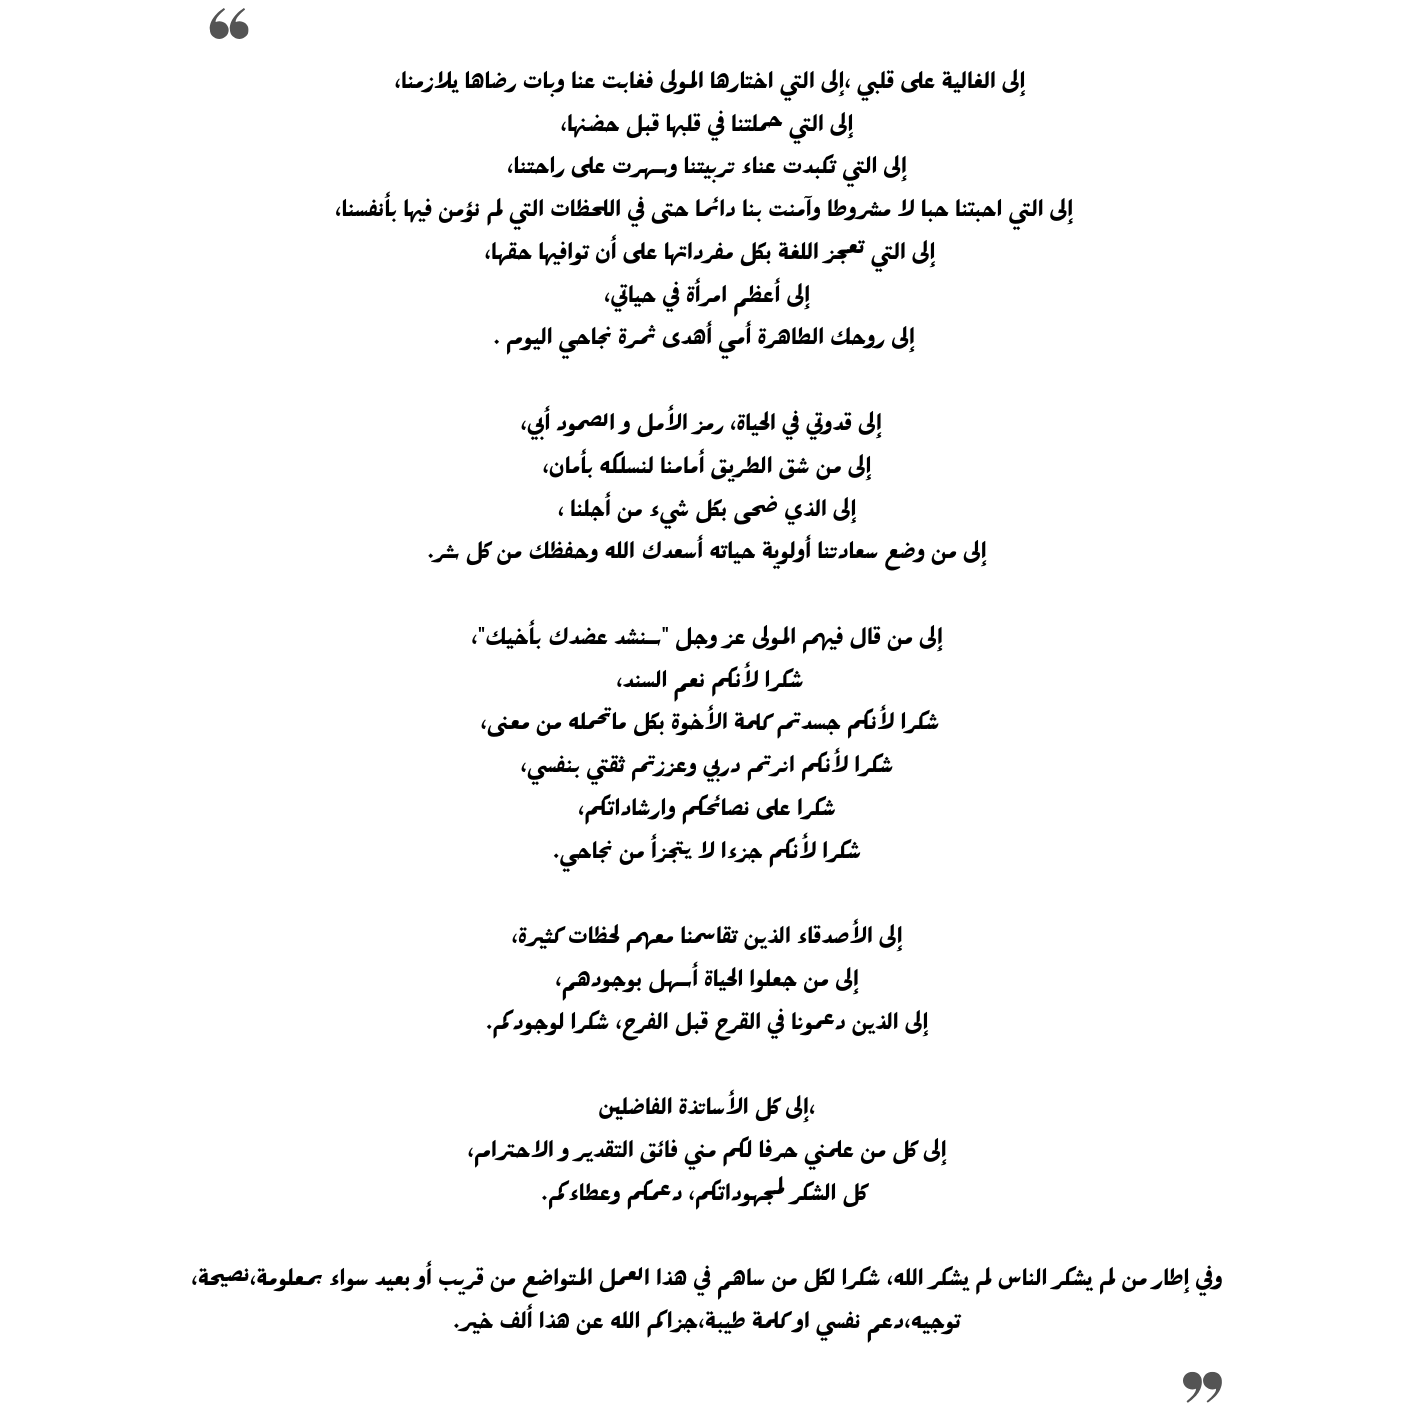
\includegraphics[width=19cm]{Figures/dedicace.png} 
\end{figure}





\chapter*{Remerciements}
\addcontentsline{toc}{chapter}{Remerciements}



Avant tout, je remercie Allah, le Tout-Puissant, de m'avoir accordé le courage et la patience nécessaires pour mener ce travail à terme dans des trés bonnes conditions.

\vspace{10pt}
Je souhaite exprimer ma gratitude à toutes les personnes qui, par leur soutien ou par leur simple présence, ont contribué à rendre mon travail à la fois instructif, bénéfique et agréable.

\vspace{10pt}
Je souhaite exprimer ma profonde gratitude à mon encadrante, \textbf{Pr. Rabiaa MARGHOUBI}, dont les connaissances, le savoir-faire et les précieuses orientations ont grandement facilité mon travail. Je lui suis reconnaissante pour ses conseils avisés, son suivi attentif, ainsi que pour la fierté et l'ambition que j'ai pu développer grâce à son soutien intensif et son aide précieuse.

\vspace{10pt}
Je souhaite également remercier chaleureusement mes encadrants externes, \textbf{Mme ELJABARI Sara} et \textbf{M. JIRARI Adil}, pour leur confiance, leur collaboration et leur soutien tout au long de mon stage. Leur supervision, leurs recommandations éclairées, leurs orientations précieuses et leur rigueur m'ont été d'une aide précieuse et ont facilité mon intégration. Je tiens aussi à adresser mes sincères remerciements aux membres de l'entreprise SQLI Maroc pour l'expérience enrichissante et captivante qu'ils m'ont offerte pendant ces mois de stage parmi eux.

\vspace{10pt}
Je tiens à exprimer ma sincère gratitude à mes examinateurs, \textbf{Pr. HAFIDDI Hatim} et \textbf{Pr. RADGUI Amina}, pour leur évaluation et leurs précieux retours. Je remercie également l'ensemble du corps enseignant de l’Institut National des Postes et Télécommunications pour leur soutien, leur expertise et leur engagement, qui ont grandement contribué à l’enrichissement de mon parcours académique.



\addcontentsline{toc}{chapter}{Moulakhass}

\begin{figure}[H]
    \thispagestyle{plain}
    \centering
    
\includegraphics[width=19cm]{Figures/abstract.png}
\end{figure}


\newpage

\chapter*{Résumé}
\addcontentsline{toc}{chapter}{Résumé}

Dans un contexte où le commerce électronique est en constante évolution, les entreprises doivent régulièrement mettre à jour et optimiser leurs plateformes pour rester compétitives. L'accélération des innovations technologiques et les attentes croissantes des consommateurs exigent une adaptation continue pour offrir des expériences utilisateur de haute qualité et répondre aux nouvelles exigences du marché. \\
\vspace{10pt}


Ce rapport présente un aperçu concis de mes contributions lors de mon stage de fin d'études effectué au sein de SQLI, dans le but d'obtenir le titre d'Ingénieur d'État en Télécommunications et Technologies de l'Information, spécialisation en Ingénierie Logicielle Avancée pour les Services Numériques à l'Institut National des Postes et Télécommunications. Ce projet avait pour objectif d'améliorer une plateforme e-commerce existante pour un client, en intégrant la méthode de paiement Payconiq spécifiquement pour le marché belge, tout en corrigeant divers bugs afin d'optimiser la performance du système.\\
\vspace{10pt}

En prenant en compte la complexité de SAP Hybris, la réalisation de ce projet a nécessité l'utilisation de technologies telles que JEE et Spring pour le développement, ainsi que JUnit pour le testing. L'intégration de Payconiq a été un défi majeur, nécessitant une attention particulière à la compatibilité et à la performance pour garantir une solution adaptée aux besoins spécifiques du marché belge.
\vspace{10pt}

\noindent\rule[2pt]{\textwidth}{0.5pt}

{\textbf{Mots clés :}}
E-commerce, Payconiq, SAP Hybris, JUnit, JEE, Spring, Déboggage
\\
\noindent\rule[2pt]{\textwidth}{0.5pt}

% % \cleardoublepage
% %

\chapter*{Abstract}
\addcontentsline{toc}{chapter}{Abstract}

In a context where e-commerce is constantly evolving, companies must regularly update and optimize their platforms to remain competitive. The acceleration of technological innovations and the growing expectations of consumers demand continuous adaptation to deliver high-quality user experience and meet new market requirements.
\vspace{10pt}

This report provides a concise overview of my contributions during my internship at SQLI Maroc, aiming to obtain the title of State Engineer in Telecommunications and Information Technologies, with a specialization in Advanced Software Engineering for Digital Services from the National Institute of Posts and Telecommunications. This project aimed to enhance an existing e-commerce platform for a prestigious client by integrating the Payconiq payment method specifically for the Belgian market, while also fixing various bugs to optimize system performance.
\vspace{10pt}

Considering the complexity of SAP Hybris, the realization of this project required the use of technologies such as JEE and Spring for development, as well as JUnit for testing. The integration of Payconiq was a major challenge, requiring particular attention to compatibility and performance to ensure a solution tailored to the specific needs of the Belgian market.
\vspace{10pt}

\noindent\rule[2pt]{\textwidth}{0.5pt}

{\textbf{Key Words :}}
E-commerce, Payconiq, SAP Hybris, JUnit, JEE, Spring, Debugging.
\\
\noindent\rule[2pt]{\textwidth}{0.5pt}

% \cleardoublepage
%

\chapter*{\begin{RLtext}{ملخص}\end{RLtext}}
\addcontentsline{toc}{chapter}{Résumé arabe}

\begin{RLtext}
 \noindent\hspace{10pt} 
 في ظل التطور المستمر الذي يشهده مجال التجارة الإلكترونية، تجد الشركات نفسها مضطرة لتحديث وتحسين منصاتها بشكل منتظم للحفاظ على قدرتها التنافسية. إذ أن تسارع الابتكارات التكنولوجية وتزايد توقعات المستهلكين يفرضان تكيفًا مستمرًا من أجل تقديم تجارب استخدام عالية الجودة وتلبية المتطلبات الجديدة للسوق.

 \vspace{10pt}

 لذا فهذا التقرير يقدم نظرة موجزة عن مساهماتي التي قدمتها في شركة \LR{"SQLI Maroc"} خلال فترة التدريب النهائي لنيل شهادة مهندس دولة في الاتصالات وتكنولوجيا المعلومات، بتخصص في هندسة البرمجيات المتقدمة للخدمات الرقمية من المعهد الوطني للبريد والمواصلات. كان الهدف من هذا المشروع تحسين منصة تجارة إلكترونية قائمة لأحد العملاء، من خلال دمج نظام الدفع \LR{"Payconiq"} خصيصًا للسوق البلجيكي، مع تصحيح مجموعة من الأخطاء البرمجية لتحسين أداء النظام.
 \vspace{10pt}

 ونظراً لتعقيد منصة \LR{"SAP Hybris"}، تطلب تنفيذ هذا المشروع استخدام تقنيات مثل \LR{"JEE"} و\LR{"Spring"} للتطوير، بالإضافة إلى \LR{"JUnit"} للاختبار. شكلت عملية دمج \LR{"Payconiq"} تحديًا رئيسيا، حيث استلزمت اهتماما خاصا بالتوافق والأداء لضمان تقديم حل يلبي الاحتياجات المحددة للسوق البلجيكي.

 \vspace{10pt}
\end{RLtext}

\noindent\rule[2pt]{\textwidth}{0.5pt}

\noindent
\begin{RLtext}
    \textbf{الكلمات المفتاحية\LR{:}} التجارة الإلكترونية،\LR{Payconiq}، \LR{SAP Hybris}، \LR{JUnit}، \LR{JEE}، \LR{Spring}، \LR{debugging}.
\end{RLtext}

\noindent\rule[2pt]{\textwidth}{0.5pt}


% \cleardoublepage
%


\chapter{Liste des sigles et acronymes}

%Example of Acronyms using table 



\begin{tabbing}
    \hspace{3cm} \= \hspace{7cm} \= \kill

    \textbf{AES} \>  Advanced Encryption Standard \\

    \textbf{API} \> Application Programming Interface \\

    \textbf{CSS} \> Cascading Style Sheets \\

    \textbf{HTML} \> HyperText Markup Language \\

    \textbf{HTTP} \> Hypertext Transfer Protocol \\

    \textbf{INPT} \> L'Institut National des Postes et Télécommunications. \\
 
    \textbf{IOS} \> IPhone Operating System \\

    \textbf{JSON} \> JavaScript Object Notation \\

    \textbf{ORDA} \> Object Relational Data Access \\

    \textbf{PAO} \> Publication Assistée par Ordinateur \\

    \textbf{REST} \> Representational State Transfer \\
 
    \textbf{SGBDR} \> Système de Gestion de Bases de Données \\

    \textbf{SGBDR} \> Système de Gestion de Bases de Données Relationnelles \\
    
    \textbf{SOA} \> Service Oriented Architecture \\

    \textbf{SQL} \> Structured Query Language \\

    \textbf{SVN} \> Subversion \\

    \textbf{UML} \> Unified Modeling Language \\
    
\end{tabbing}




\listoffigures
\addcontentsline{toc}{chapter}{Table des figures} 
%figures are added automatically here

\listoftables
\addcontentsline{toc}{chapter}{Liste des tableaux} 
%tables are added automatically here



\tableofcontents
\addcontentsline{toc}{chapter}{Table des matières}
%contents are added automatically here



\mainmatter

\chapter*{Introduction générale}
\addcontentsline{toc}{chapter}{Introdcution}


Dans un environnement numérique en perpétuelle évolution, où les attentes des consommateurs et les technologies avancent rapidement, il est crucial pour les entreprises d'améliorer continuellement leurs plateformes e-commerce afin de rester compétitives. Ce projet de fin d'études s'inscrit dans ce contexte dynamique, en visant à améliorer une plateforme e-commerce pour un client spécifique et à intégrer la méthode de paiement Payconiq, particulièrement pertinente pour le marché belge.

\vspace{10pt}

L’objectif principal de ce projet est de moderniser la plateforme en ajoutant Payconiq comme nouvelle méthode de paiement, afin d'optimiser l'expérience utilisateur et de répondre aux exigences locales. Ce rapport se compose de quatre chapitres distincts : 

Le premier chapitre présente le contexte général du projet, en détaillant l'organisme d'accueil, l'équipe impliquée, la problématique identifiée, les objectifs visés, ainsi que la méthodologie de travail adoptée. 

Le deuxième chapitre est dédié à l'analyse de l'existant et à l'étude des besoins fonctionnels et non fonctionnels, en mettant en lumière les spécificités actuelles de la plateforme et les exigences liées à l'intégration de Payconiq.

Le troisième chapitre se concentre sur la conception du projet, illustrée par les diagrammes UML qui décrivent les structures et les interactions au sein de la plateforme.

Enfin, le quatrième chapitre traite de la réalisation du projet, en détaillant le processus d'implémentation de la nouvelle méthode de paiement et en évaluant son impact sur la plateforme.

\vspace{10pt}

Ce rapport fournit une vue d'ensemble complète de l'amélioration de la plateforme e-commerce et de l'intégration de Payconiq, tout en offrant des perspectives pour les développements futurs.


%debut of chapters

\chapter{Contexte général du projet}
\label{chap:Contexte général du projet}



Ce chapitre situe mon projet de fin d’études dans son environnement organisationnel et contextuel. Il commence par une présentation de l’organisme d’accueil, SQLI Maroc. Ensuite, il détaille la problématique ayant conduit à la réalisation de ce projet ainsi que les objectifs visés. Enfin, la méthodologie adoptée pour mener à bien le projet est abordée.

\newpage


\section{Présentation de l’entreprise d’accueil SQLI}

Cette section initiale met en lumière le Groupe SQLI en mettant l’accent sur ses activités clés, son
chiffre d’affaires ainsi que ses clients. Ensuite, l'accent sera mis sur SQLI Maroc, en mettant en avant ses valeurs fondamentales.

\subsection{Groupe SQLI}

\begin{figure}[h]
    \centering
    
\includegraphics[scale=0.7]{Logos/SQLI_LOGO.png} % Replace with the actual filename of the IBM logo image
    \caption{Logo de SQLI \cite{SQLI}}
    \label{fig:LogoSQLI}
\end{figure}

SQLI est une entreprise européenne de services numériques fondée en 1990 par Jean Rouveyrol et Alain Lefebvre. Elle se spécialise dans la conception, le développement et le déploiement de solutions digitales
visant à créer des expériences unifiées \cite{SQLI}. Avec un effectif de 2400 collaborateurs répartis dans 13 pays,
SQLI bénéficie d’une présence internationale solide.

Le succès de SQLI Digital Experience repose sur des valeurs fondamentales telles que la créativité, l'engagement et l'audace visionnaire. Ces valeurs imprègnent chaque aspect de l'entreprise, permettant de repousser les frontières de l'innovation et de concevoir des expériences digitales uniques et captivantes. \cite{valeurSQLI}

\subsubsection{Activités du groupe} 

Le groupe SQLI propose une gamme étendue de services pour accompagner les entreprises dans leur transformation numérique. Il inclut l'e-commerce, créant et optimisant des plateformes de vente en ligne performantes. Il offre également des plateformes d'expérience, conçues pour offrir des interactions utilisateur exceptionnelles. En matière de technologie et de transformation, il aide les entreprises à moderniser leurs infrastructures et leurs processus. Ses services de data et insights permettent d'exploiter les données de manière stratégique, tandis que son expertise en marketing digital et design améliore la visibilité et l'attrait des marques. Enfin, son conseil digital guide les entreprises dans l'élaboration et la mise en œuvre de leur stratégie numérique globale, assurant ainsi une transformation digitale réussie. \cite{SQLI}

\subsubsection{Chiffres Clés du groupe}

Les chiffres clés suivants présentent la situation actuelle de SQLI :

\begin{itemize}
    \item[$\bullet$] Fort de 33 ans d’expérience et d’innovation, SQLI fonde son développement sur une expertise technologique de pointe et une politique de veille intensive.
    \item[$\bullet$] SQLI emploie plus de 2400 collaborateurs répartis dans 13 pays, notamment la France, l'Angleterre, la Suède, les Pays-Bas, l'Espagne, l'Allemagne, la Belgique, le Luxembourg, la Suisse et le Maroc.
    \item[$\bullet$] En 2022, le groupe SQLI a atteint un chiffre d’affaires de 251,2 millions de dollars. Ce succès est le résultat d'une offre bien alignée sur les attentes du marché et d'une reprise progressive de la demande de services informatiques.
    \vspace{0.5cm}
\end{itemize}

\begin{figure}[H]
    \centering
    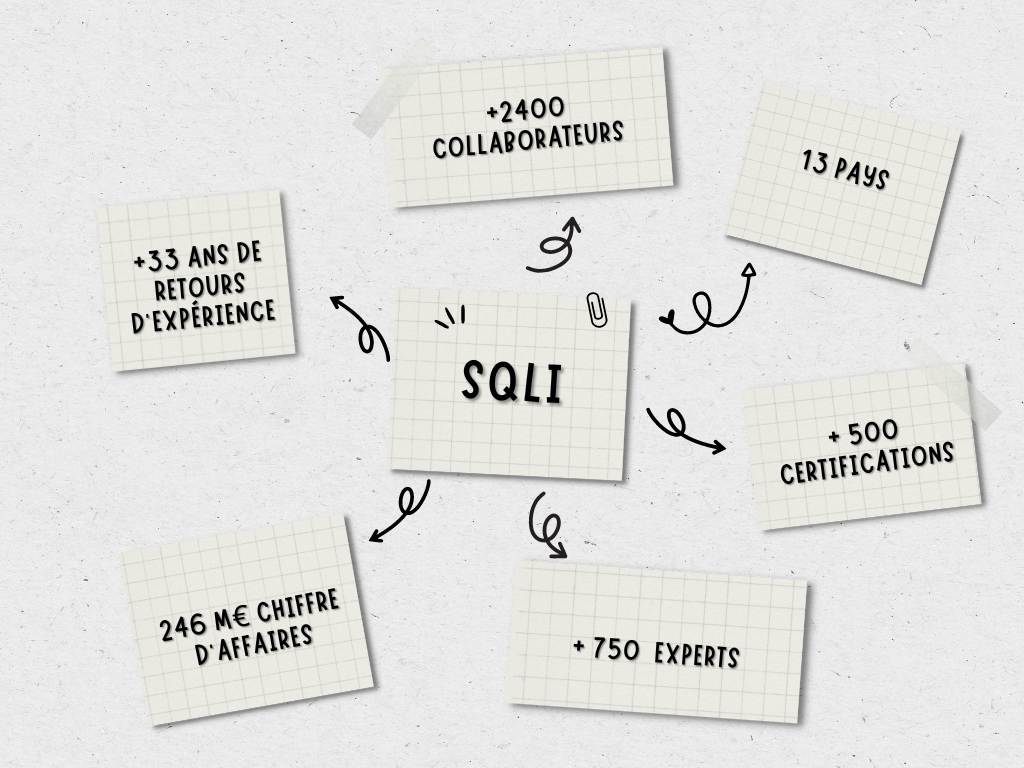
\includegraphics[width=10cm]{Figures/cle chiffre.png} % Replace with the actual filename of the IBM logo image
    \caption{Chiffre Clés de SQLI}
\end{figure}

\subsubsection{Clients du groupe}

SQLI collabore avec une vaste gamme de clients provenant de divers secteurs, y compris l'automobile, la distribution, la banque et l'assurance, le luxe et la mode, la santé, l'industrie et l'énergie, ainsi que les télécommunications. Les grandes entreprises internationales et les organisations locales font appel à SQLI pour ses solutions digitales innovantes, allant de l'optimisation des plateformes d'e-commerce à la transformation numérique des services financiers, en passant par la création d'expériences utilisateur uniques pour les marques de luxe et la digitalisation des processus industriels. Grâce à sa capacité à répondre aux besoins spécifiques de chaque secteur, SQLI bâtit des partenariats solides et durables avec ses clients (\textit{Figure~\ref{fig:client}})

\begin{figure}[H]
    \centering
    
\includegraphics[width=15cm]{Figures/sqli partenaire .png} % Replace with the actual filename of the IBM logo image
    \caption{Clients du SQLI \cite{SQLI}}
    \label{fig:client}
\end{figure}


\subsection{SQLI Maroc}

SQLI Maroc, créée en 2003 à Rabat par Eric Chanal, représente le centre de Delivery et d'Innovation du Groupe SQLI. Bénéficiant d'une solide expertise et d'une grande expérience, l'entreprise est présente sur trois sites stratégiques : Rabat, où j'ai eu l'opportunité d'effectuer mon stage PFE, Oujda et Casablanca. Le tableau \textit{\ref{tab:fiche}} représente sa fiche technique:



% l'ajoute de titre de tableau avec space between titre de tab et le tab
% \captionsetup{type=table}

% \vspace{0.3cm}
% tab
\begin{center}
    \captionsetup{type=table}
    \vspace{0.3cm}
    \begin{tabularx}{17cm}{|X|X|}
      \hline
     \textbf{Dénomination sociale}  & \textbf{SQLI Digital Experience} \\
      \hline
     {Année de fondation} & 2003  \\
      \hline
      {Fondateur} & Eric Chanal  \\
      \hline
     {Siège social} & Rabat, Maroc\\
     \hline  
     {Activité} & Conseil en systèmes et logiciels informatiques.\\
      \hline  
     {Effectif des employés} & Plus de 900 collaborateurs.\\
      \hline
     {Sites d'implantation} & Rabat, Oujda et Casablanca.\\
      \hline
    \end{tabularx}
    \captionof{table}{Fiche technique de SQLI Maroc}
    \label{tab:fiche}
    \end{center}
    

  SQLI Maroc comprend principalement deux structures essentielles, présentées dans la \textit{Figure~\ref{fig:departement}}, à savoir :

\begin{enumerate}
    \item \textbf{SQLI WAX INTERRACTIVE} : accompagne les clients dans leur transition vers la digitalisation afin de renforcer leur positionnement sur le marché. Cette entité intervient principalement sur le plan stratégique en collaborant étroitement avec les clients.
     \item \textbf{SQLI ENTREPRISE} : est chargée de la mise en œuvre des systèmes d'information pour les clients. Elle se compose de plusieurs Business Units spécialisées dans différents domaines :
\begin{itemize}

    \item [$\bullet$]\textbf{E-commerce/ JAVA EE} : Se focalise sur la création et la mise en place de sites de e-commerce ainsi que sur le développement d’applications utilisant la technologie Java EE.
    \item [$\bullet$]\textbf{Mobile/Front} : Se spécialise dans le développement d’applications mobiles et l’interface utilisateur (front-end) pour les clients.
    \item [$\bullet$]\textbf{Microsoft} : S'occupe de la réalisation d’applications basées sur les technologies Microsoft.
    \item [$\bullet$]\textbf{Agency} : Joue un rôle transversal en assurant la conception de l’interface utilisateur (front-end) pour toutes les autres Business Units.
    \item [$\bullet$]\textbf{Delivery} : Se charge de la gestion des livraisons et des recettes auprès des clients.
\end{itemize}
\end{enumerate}
\vspace{0.5cm}
\begin{figure}[H]  
  \centering  
  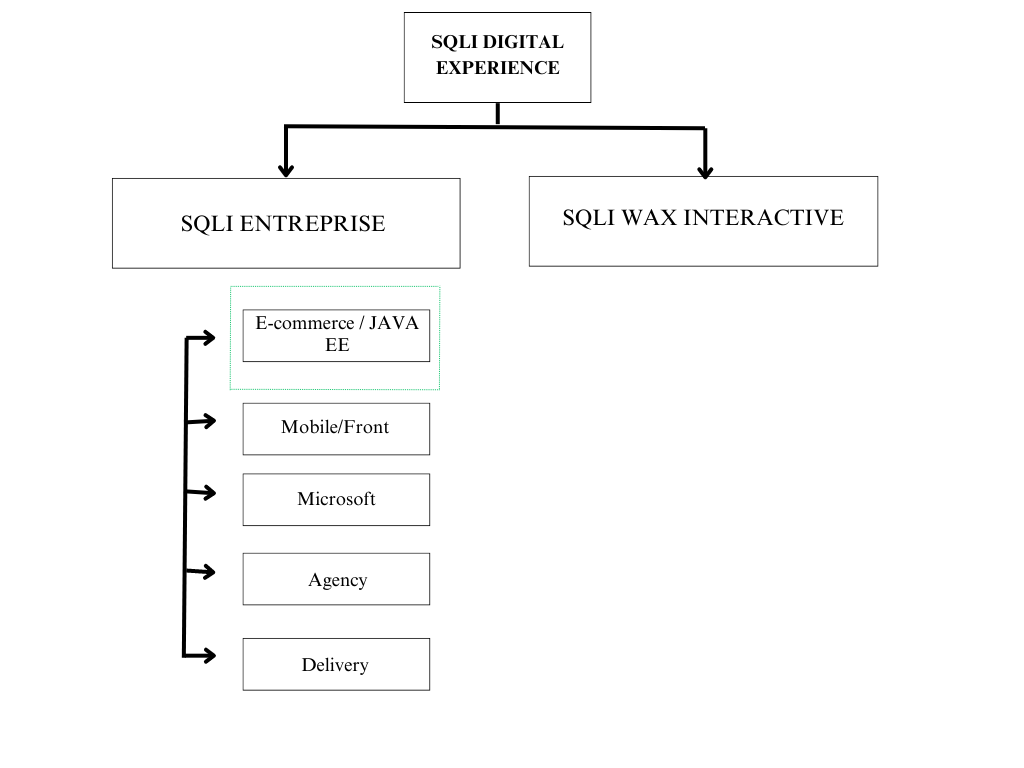
\includegraphics[width=14cm]{Figures/departement.png}
  \caption{Départements de SQLI}
  \label{fig:departement}
\end{figure}


Mon stage de fin d'études s'est déroulé dans le département Java JEE, qui regroupe plusieurs projets destinés à des grandes entreprises clientes.


\section{Présentation du projet}

\subsection{Cadre du projet et problématique}

Dans le cadre d'un projet e-commerce pour un client de luxe, l'objectif est d'améliorer et d'optimiser sa plateforme actuelle. Il est indispensable de mettre à jour régulièrement cette plateforme, qui joue un rôle crucial dans les activités commerciales en ligne du client, afin de maintenir sa compétitivité et de répondre aux exigences du marché.

Pour cette amélioration, le travail inclut la correction de divers bugs qui affectent la performance et la fiabilité du système. La résolution de ces bugs est cruciale pour garantir une expérience utilisateur fluide et sans interruptions.

En parallèle, l'intégration de nouvelles fonctionnalités est nécessaire pour enrichir l'offre de la plateforme. L'un des changements majeurs est l'intégration de la méthode de paiement Payconiq, destinée spécifiquement au marché belge. Différents défis se posent lors de cette intégration, tels que la compatibilité avec l'architecture existante, la gestion des dépendances et l'assurance que cette nouvelle fonctionnalité ne provoque pas de régressions ou de nouveaux bugs.

L'enjeu majeur consiste donc à corriger les bugs existants tout en intégrant Payconiq de manière efficace, en maintenant la stabilité et la performance globale de la plateforme.

 \subsection{Objectifs du projet}

 Dans le cadre de ce projet, je participerai activement aux diverses activités de l'équipe, contribuant à la fois au développement des fonctionnalités demandées par le client et à l'amélioration continue du système. Les objectifs spécifiques de mon intervention sont les suivants :

 \begin{itemize}
    \item[$\bullet$] \textbf{Intégrer un nouveau mode de paiement, Payconiq, pour le marché belge } 
    
    Analyser et comprendre l'architecture existante pour intégrer Payconiq, tout en gérant les dépendances et en garantissant la compatibilité avec les autres modules de la plateforme, conformément aux spécificités techniques du marché belge. Cela inclut la configuration, le développement, et des tests rigoureux pour garantir une intégration fluide dans les différents flux de paiement existants.

    \item[$\bullet$] \textbf{Assurer les livraisons dans différents environnements (DEV, INTx, UAT, PRD) } 
    
    Garantir le bon fonctionnement du code dans chacun de ces environnements, conformément aux exigences de stabilité et de performance. Cela comprend des tests approfondis pour s'assurer que les nouvelles fonctionnalités et intégrations sont stables et opérationnelles avant la mise en production.

    \item[$\bullet$] \textbf{Respecter les meilleures pratiques, les normes, et l'architecture du projet } 
    
    Assurer la cohérence du code et la stabilité du projet en adhérant aux normes et pratiques de développement établies. Cela inclut le respect des principes d'architecture définis, l'application des bonnes pratiques de codage, et la proposition de solutions conformes aux standards en vigueur au sein de l'équipe.

    \item[$\bullet$] \textbf{Analyser et corriger les bugs détectés }
    
    Assurer la maintenance corrective du système en identifiant, analysant, et résolvant les bugs remontés par les équipes du projet ou découverts lors des tests, afin de minimiser leur impact sur le fonctionnement global de la plateforme.

\end{itemize}

 %%%%%%%%%%%%%%%%%%%% SECTION 4 %%%%%%%%%%%%%%%%%%%%%%%
\section{Conduite de projet}

\subsection{Présentation des équipe du projet}

Après ma période de formation, j’ai intégré une première équipe en tant que stagiaire backend. Cette équipe était responsable de la gestion des fonctionnalités de recherche, un élément crucial permettant aux utilisateurs de trouver efficacement des produits au sein de la plateforme, ainsi que des aspects spécifiques aux lunettes, incluant des filtres de sélection basés sur les formes et types de montures, et de la mode. À mon arrivée, l'équipe se concentrait sur le Plan 99.5, visant à analyser les bugs, nettoyer les logs, corriger les erreurs et refactoriser le code. La structure de cette équipe, nommée Seasonal Event, est illustrée dans la \textit{Figure~\ref{fig:structure_seasonal_event}}.

Souhaitant approfondir mes compétences dans des domaines complémentaires, j'ai ensuite rejoint une autre équipe, chargée de l’intégration des nouvelles méthodes de paiement pour les différents marchés du client. La structure de cette équipe, nommée Cart Checkout \& Payment, est illustrée dans la \textit{Figure~\ref{fig:structure_payment}}.

Ces deux équipes font partie d'un projet plus vaste comprenant 15 équipes fonctionnelles différentes. Chaque équipe est composée d'un Scrum Master, d'un expert technique, d'un Product Owner, d'un développeur frontend et de deux responsables qualité, favorisant ainsi le développement d'une solution robuste et performante.

\begin{center}
    \centering
    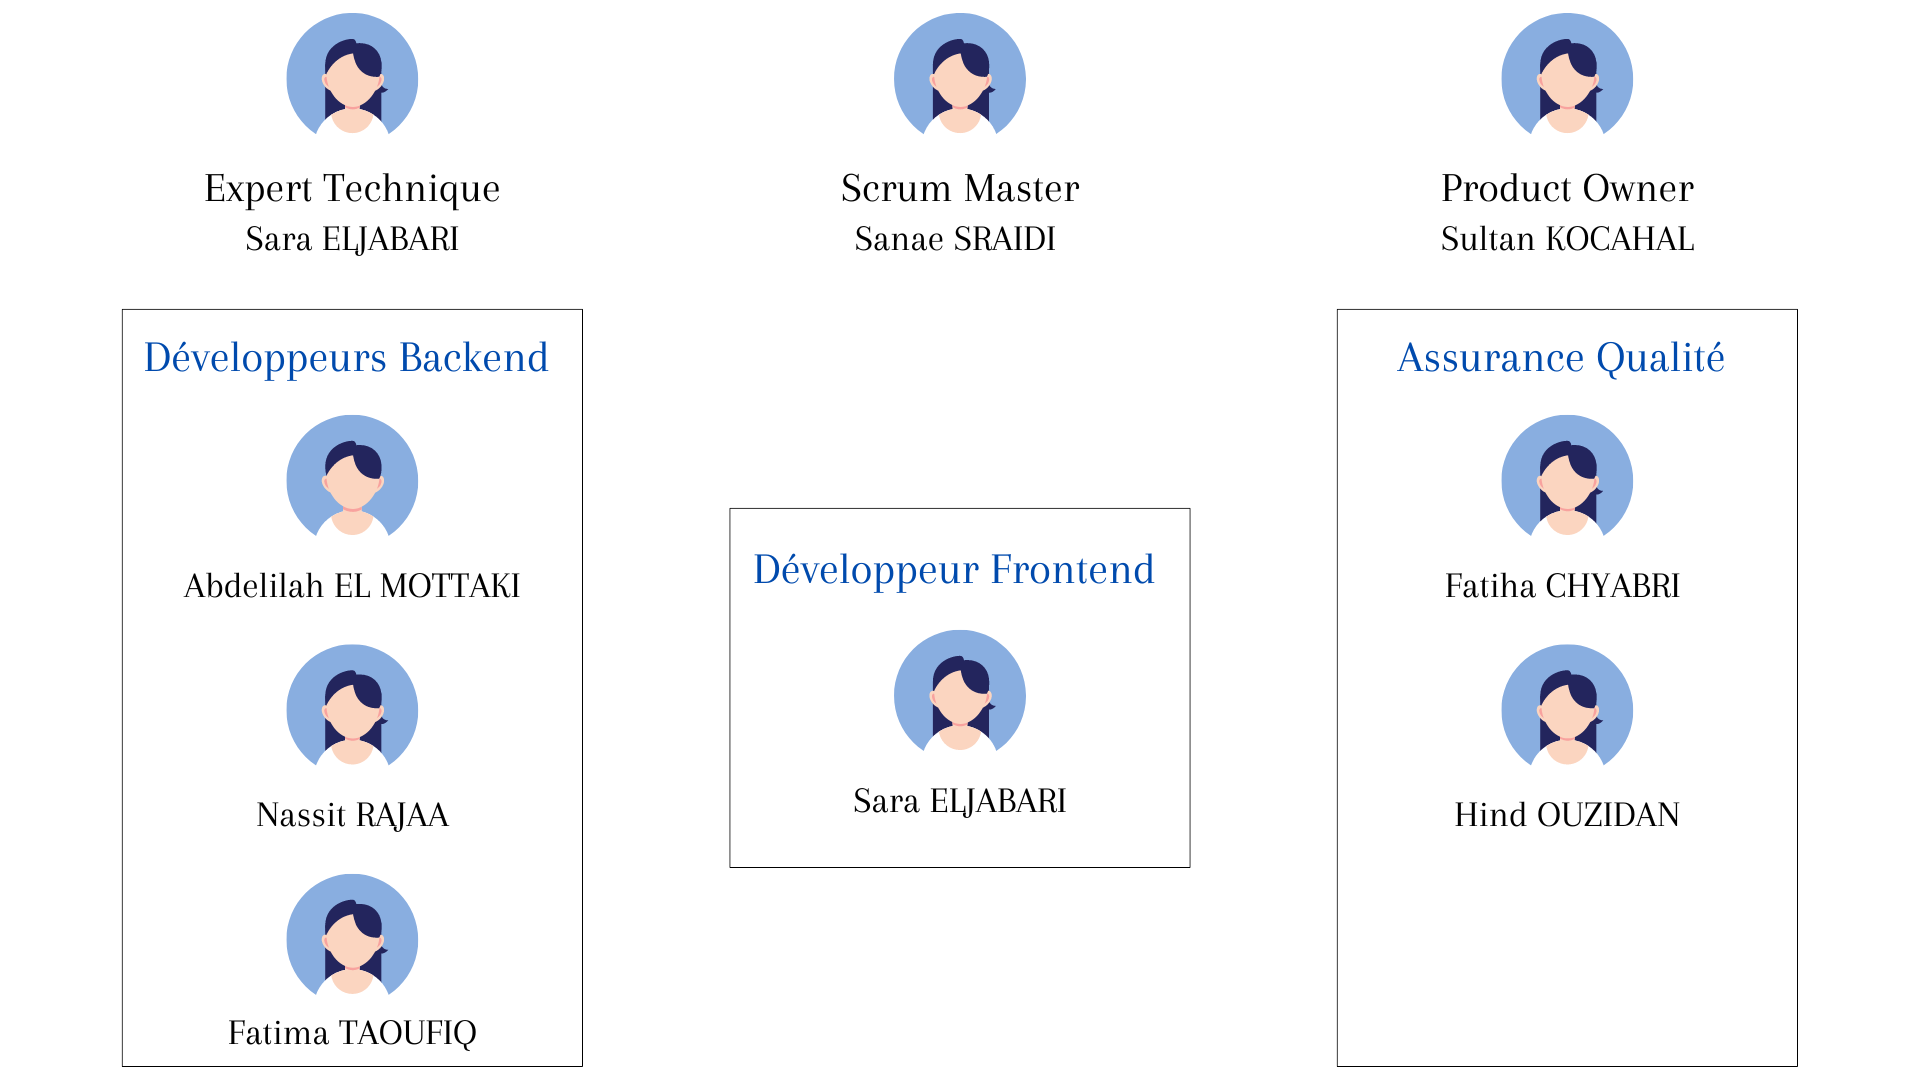
\includegraphics[width=19cm]{Figures/Seasonal Event Team.png}
    \captionof{figure}{Structure de l'équipe Seasonal Event}
    \label{fig:structure_seasonal_event}
\end{center}

\begin{center}
    \centering
    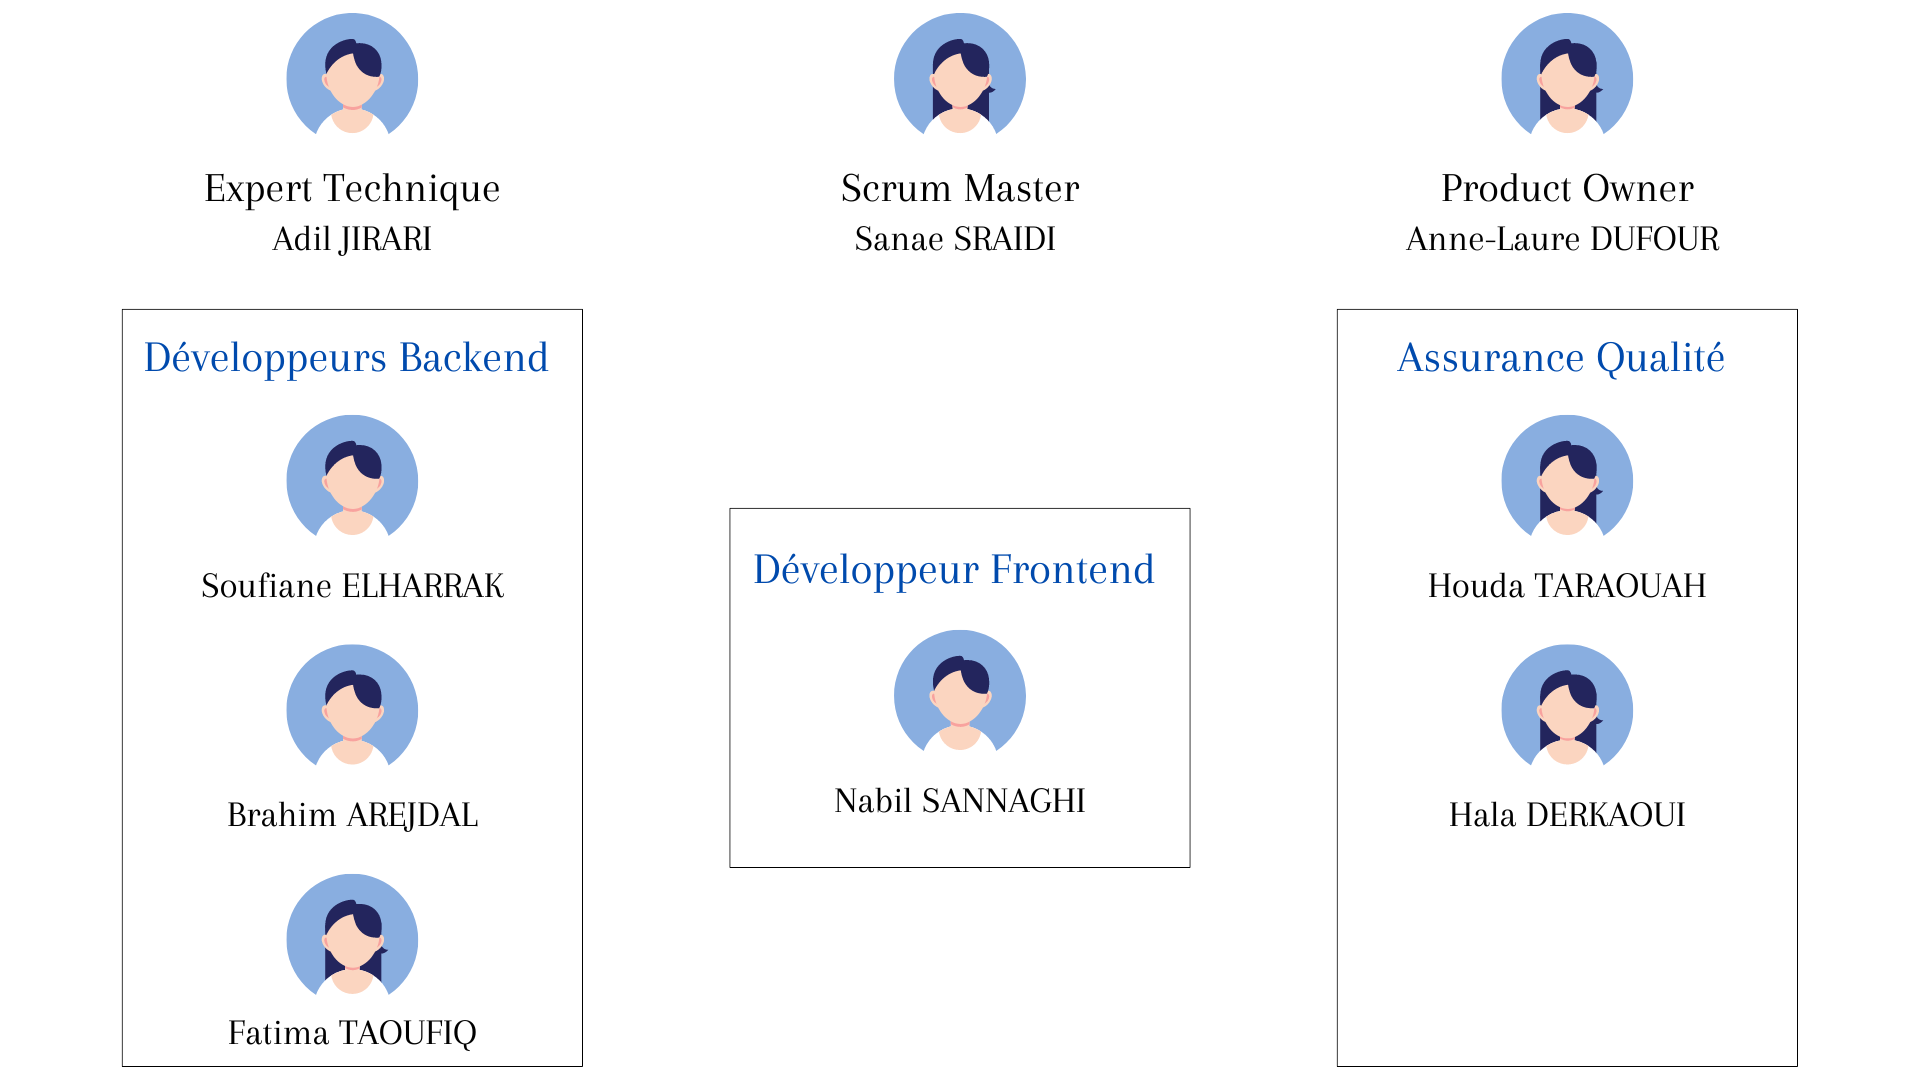
\includegraphics[width=19cm]{Figures/Cart Checkout & Payment.png}
    \captionof{figure}{Structure de l'équipe Cart Checkout \& Payment}
    \label{fig:structure_payment}
\end{center}


\subsection{Méthodologie de travail : Scrum}

Pour assurer une collaboration efficace au sein de l'équipe, nous avons opté pour la méthodologie Scrum, qui se caractérise par une approche itérative et incrémentale. Scrum nous permet de diviser le travail en sprints, des cycles de développement courts et cadencés, généralement de deux à quatre semaines. À la fin de chaque sprint, une version potentiellement livrable du produit est présentée, ce qui favorise la flexibilité et l'adaptation aux changements. Grâce à cette méthode, nous pouvons rester réactifs et ajuster rapidement notre travail en fonction des évolutions des besoins métiers. En intégrant les retours d'expérience du client à chaque itération, nous assurons une satisfaction optimale de ses attentes. Les rôles bien définis, tels que le Scrum Master, le Product Owner, et l'équipe de développement, garantissent une communication claire et une responsabilité partagée. Cette approche nous permet d'être efficaces tout en maintenant un rythme de travail soutenu et structuré.


\textbf{\textbullet \textit{Planification du sprint (sprint planning)}}

Avant de débuter chaque sprint, nous tenons une réunion de Sprint Planning. Cette réunion a pour objectif de définir les tâches prioritaires à accomplir au cours du sprint à venir. L'équipe, en collaboration avec le Product Owner, examine le backlog du produit pour identifier les éléments les plus critiques à traiter. Durant cette session, nous discutons des exigences, des objectifs du sprint, et nous évaluons la charge de travail nécessaire pour chaque tâche. Cette planification permet à l'équipe de se concentrer sur un ensemble de fonctionnalités claires et réalisables, tout en s'assurant que les ressources sont allouées de manière optimale. Ainsi, chacun sait précisément sur quoi se concentrer, ce qui contribue à une exécution efficace et coordonnée du sprint.

\textbf{\textbullet \textit{Mêlée quotidienne (Daily Meeting)}}

Chaque jour, nous tenons une réunion appelée Daily Meeting, d'une durée de 15 minutes chaque matin. Lors de cette réunion, chaque membre de l'équipe partage ce qu'il a accompli la veille, ce qu'il prévoit de faire aujourd'hui, et signale s'il rencontre des problèmes ou des blocages. Cette réunion permet à l'équipe de rester synchronisée et d'identifier rapidement les obstacles éventuels, favorisant ainsi une meilleure collaboration et une résolution rapide des problèmes.

\textbf{\textbullet \textit{Revue de sprint (Sprint Review) }}

La revue de sprint se tient à la fin de chaque sprint pour présenter et évaluer les fonctionnalités développées. L'équipe démontre le travail accompli aux parties prenantes, recueille leurs retours et discute des ajustements nécessaires. Ce moment est crucial pour valider les résultats, s'assurer qu'ils répondent aux attentes et planifier les prochaines étapes en fonction des feedbacks reçus.

\textbf{\textbullet \textit{Rétrospective de sprint }}

À la fin de chaque sprint, nous tenons une rétrospective de sprint, un moment privilégié pour discuter des succès et des aspects à améliorer dans notre travail. Pour détendre l'atmosphère et réduire le stress, nous intégrons également de petits jeux qui permettent de sortir de la routine, de mieux connaître les membres de l'équipe, et de renforcer notre cohésion. Ces activités, combinées à des discussions constructives, nous aident à identifier les points à optimiser et à faire évoluer nos pratiques de manière continue.

\textbf{\textbullet \textit{Préparation du backlog (Backlog Refinement) }}

Nous tenons régulièrement des réunions de préparation du backlog, également appelées sessions d'affinement du backlog. Lors de ces réunions, l'équipe Scrum se réunit pour examiner et ajuster les éléments du backlog du produit. Nous clarifions les exigences, estimons les efforts nécessaires pour chaque tâche, et réorganisons les priorités en fonction des retours des parties prenantes et des évolutions du projet. Cette réunion est essentielle pour maintenir le backlog bien structuré et aligné avec les objectifs du projet, ce qui facilite une planification plus efficace des sprints et assure une gestion optimale des priorités.


\subsection{Capitalisation et suivi}

Pour assurer un suivi efficace du projet, l'équipe utilise des outils de gestion de projet tels que Azure DevOps et Confluence.

\textbf{\textbullet \textit{ Confluence}}

Confluence est utilisé pour la documentation et l'archivage des informations du projet, offrant une base de connaissances centralisée accessible à tous les membres de l'équipe. Cette plateforme permet de créer, organiser et maintenir des documents essentiels tels que les spécifications techniques, les guides de processus et les comptes rendus de réunions. En centralisant ces informations dans Confluence, nous facilitons la réutilisation des connaissances et assurons leur préservation au-delà de la durée du projet. Cette approche améliore la transparence, soutient la collaboration et garantit que les informations cruciales sont facilement accessibles pour toute l'équipe.

\begin{center}
    \centering
    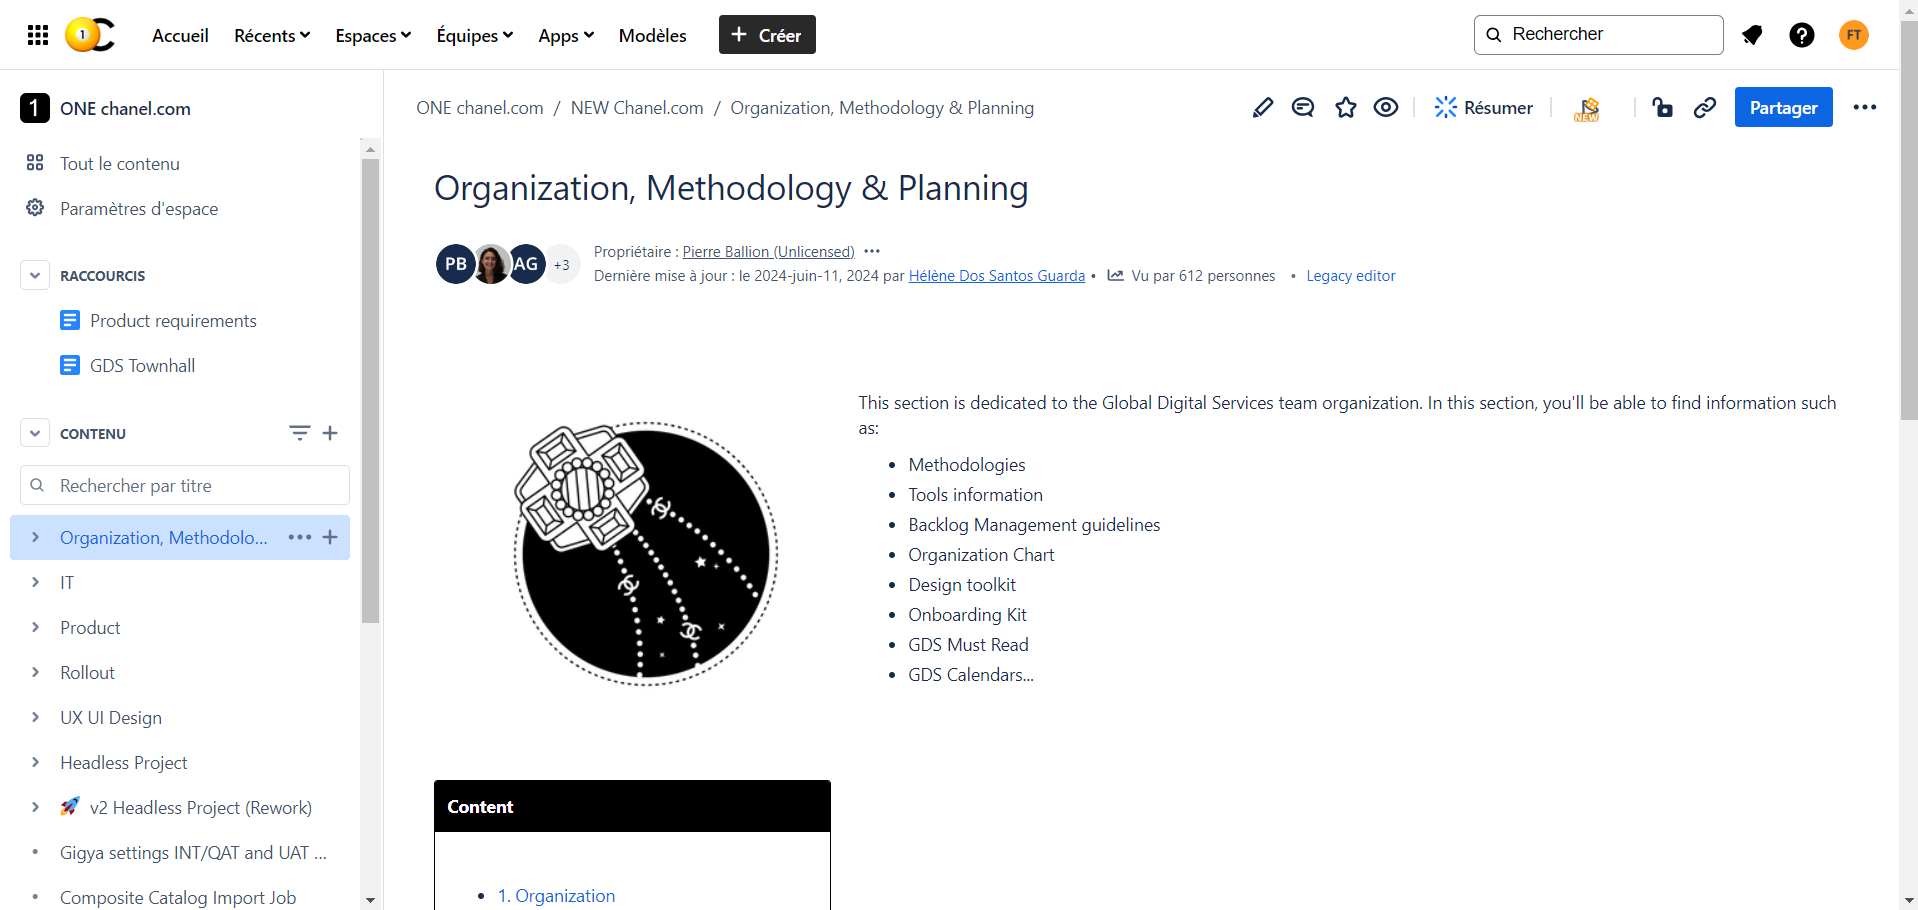
\includegraphics[width=19cm]{Figures/Confluence Documentation.png}
    \captionof{figure}{Page d’accueil de Confluence}
\end{center}


\textbf{\textbullet \textit{Azure DevOps}}

Azure DevOps nous permet de gérer efficacement les tâches à réaliser et de suivre en temps réel l'avancement de chaque membre de l'équipe. En plus de ces fonctionnalités de gestion de projet, Azure DevOps sert également de dépôt centralisé pour le code et les artefacts du projet, facilitant ainsi la collaboration et l'intégration continue.
\begin{center}
    \centering
    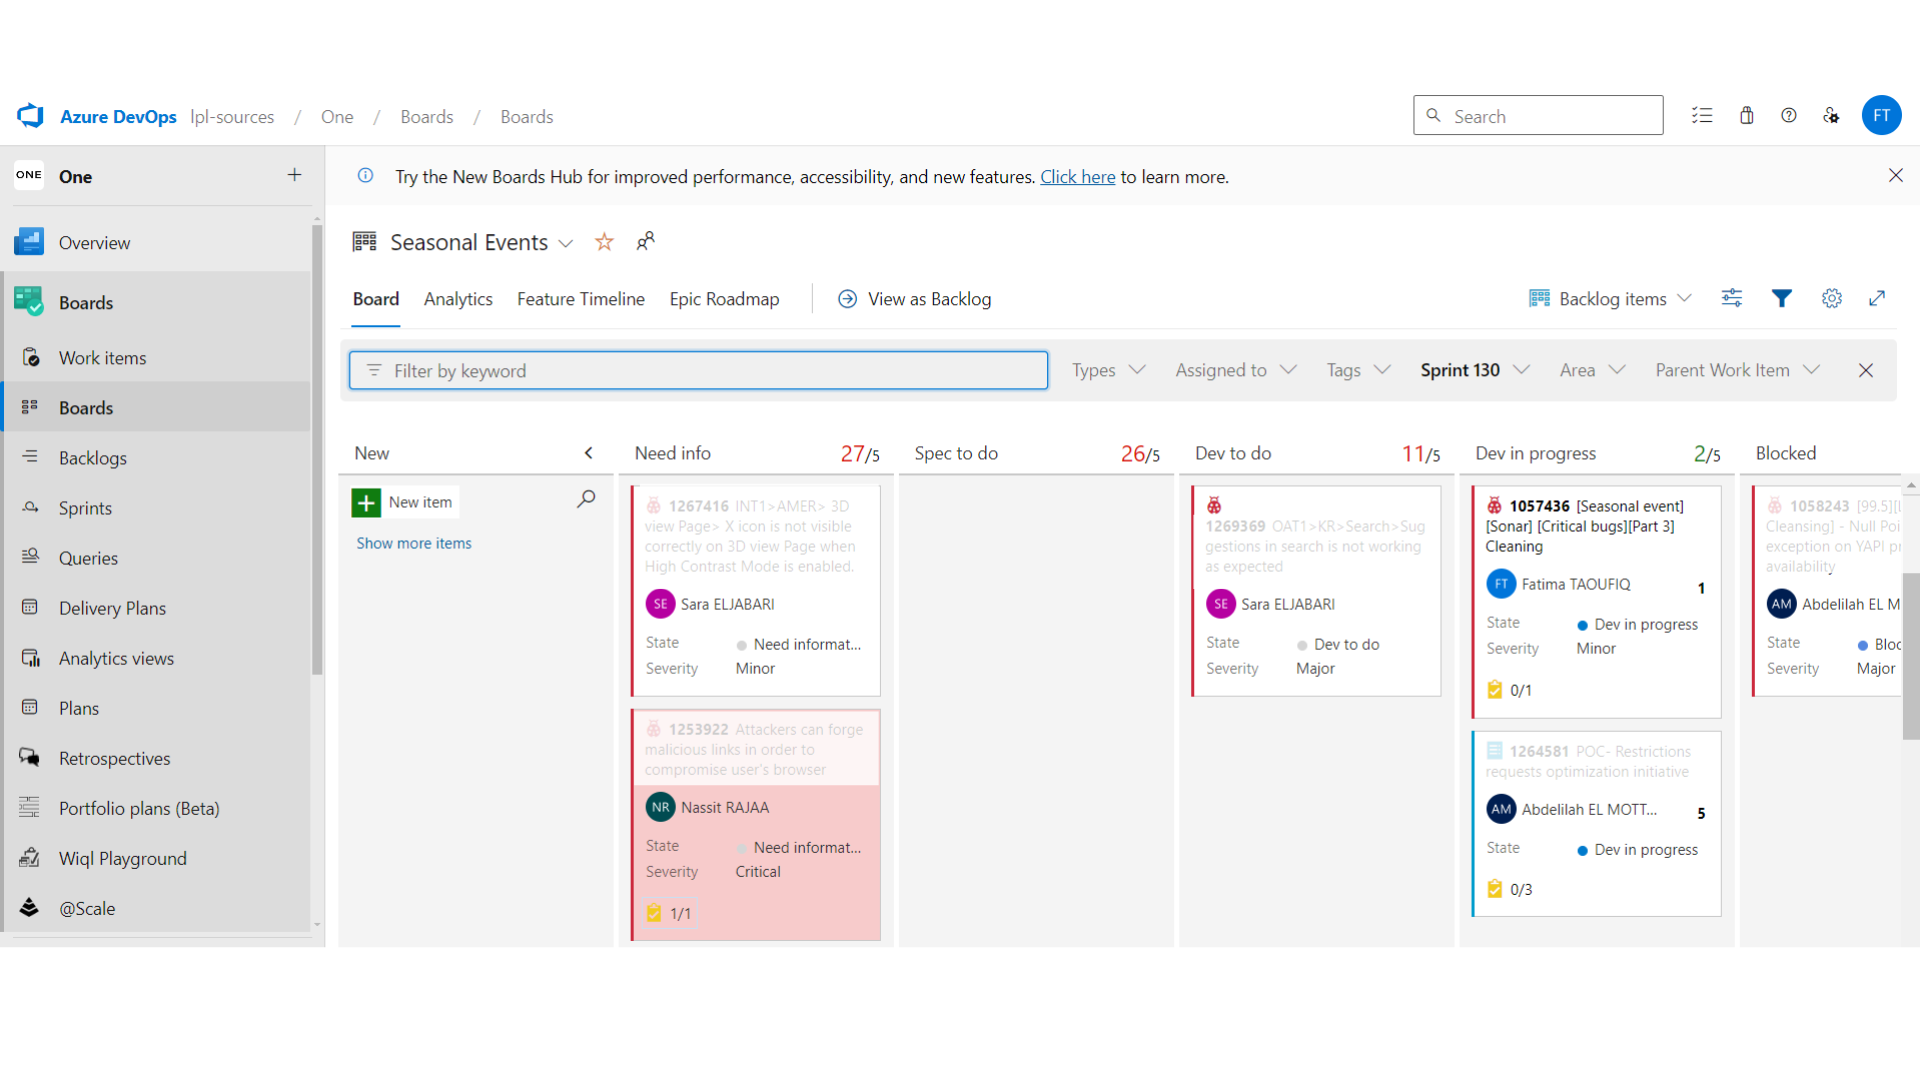
\includegraphics[width=18cm]{Figures/azure DevOps-tickets.png}
    \captionof{figure}{Backlog du projet sur Azure DevOps}
\end{center}

\textbf{\textbullet \textit{Microsoft Teams}}

Microsoft Teams est un outil essentiel pour la communication et la collaboration au sein du projet. Il nous permet de maintenir une communication fluide entre les managers, les chefs de projet, et les membres de l'équipe. Lorsqu'il est nécessaire de contacter quelqu'un pour obtenir des informations, poser des questions ou résoudre des problèmes, j'utilise Teams pour envoyer des messages instantanés, organiser des réunions virtuelles ou partager des documents. Cet outil facilite également la coordination des tâches et le suivi des progrès en centralisant les échanges et les informations pertinentes, ce qui contribue à une gestion de projet efficace et une meilleure intégration des membres de l'équipe.


\subsection{Planification du projet}
\subsubsection{Formation}
Durant les deux premiers mois du stage, des formations spécifiques ont été dispensées afin d'assurer une montée en compétences dans les technologies clés utilisées sur le projet. Ces formations ont couvert plusieurs domaines techniques et méthodologiques essentiels, tels que :
\begin{center}
    \centering
    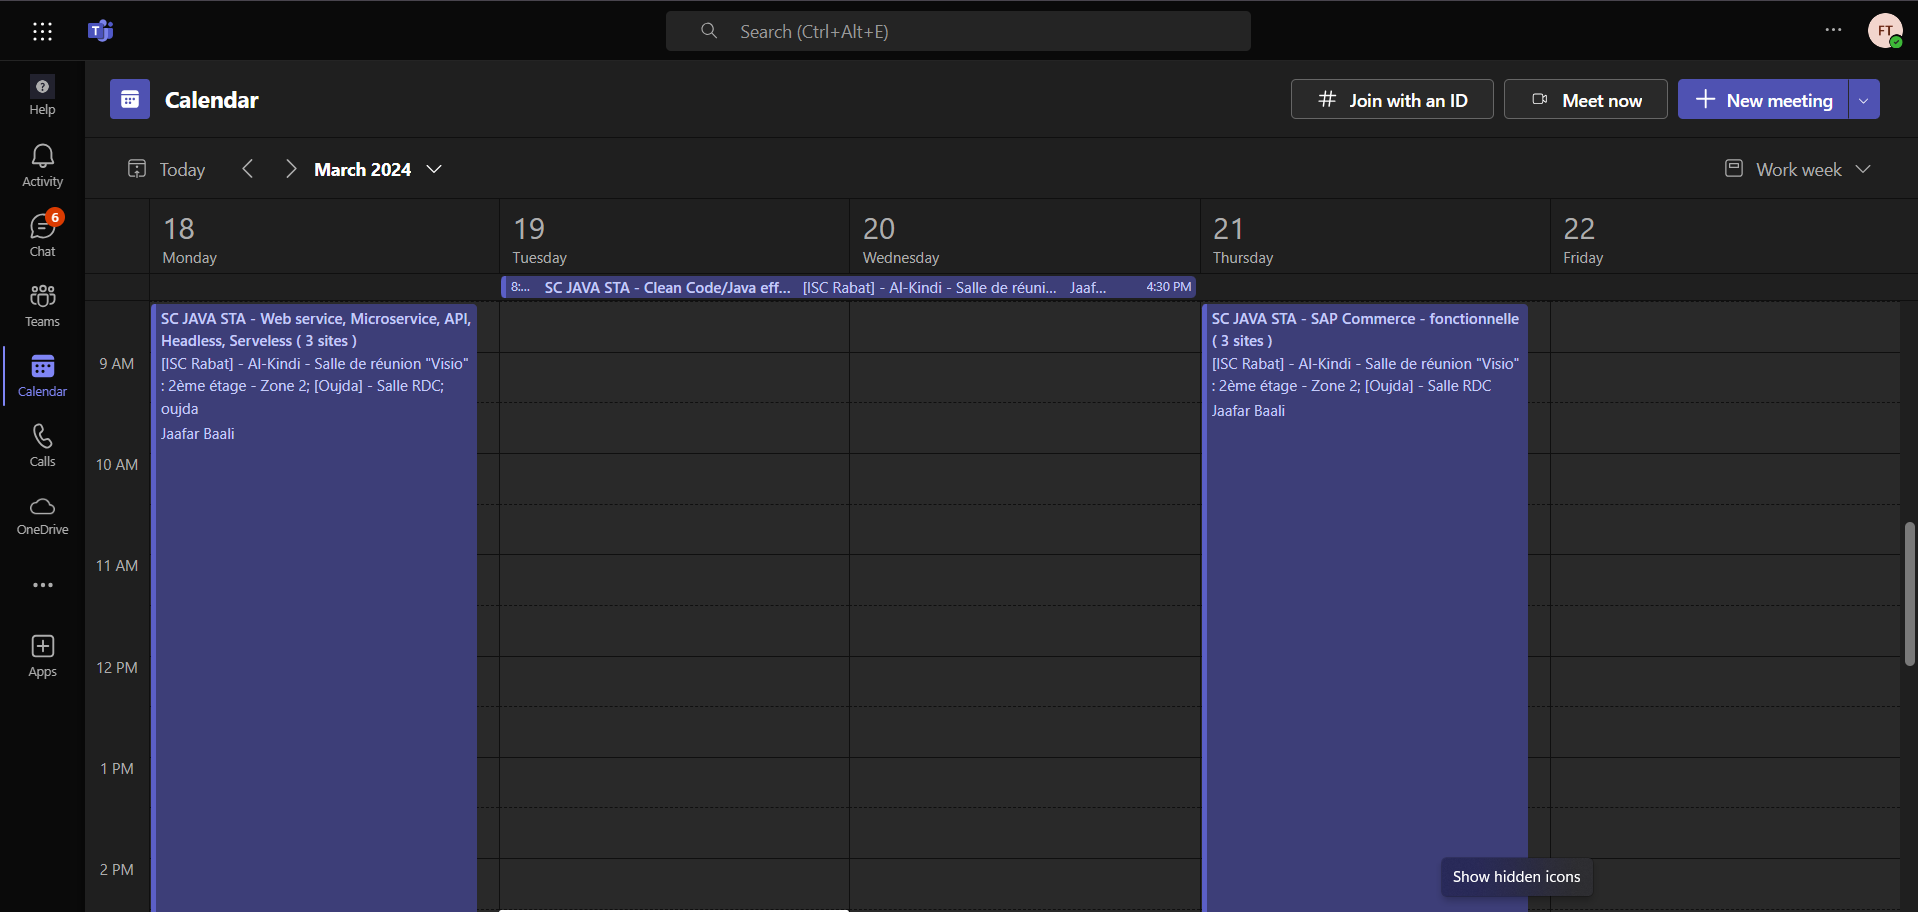
\includegraphics[width=19cm]{Figures/formation.png}
    \captionof{figure}{Calendrier des formations}
    \label{fig:structure_payment}
\end{center}
\begin{itemize}
    \item \textbf{\textit{Formations Spring :}}
    La formation sur Spring Framework a abordé les concepts fondamentaux, tels que l'inversion de contrôle (IoC) et Spring MVC. Ces notions ont été approfondies à travers des exercices pratiques, permettant de comprendre l'architecture et le fonctionnement des applications Java développées avec ce framework.
    \item \textbf{\textit{SAP Commerce (Hybris) :}} Ce volet a débuté par l’installation de la plateforme SAP Commerce. Les outils d’administration, tels que HAC, HMC et les Cockpits, ont ensuite été explorés, ainsi que les fonctionnalités techniques, notamment la configuration de CronJobs et la gestion des workflows.    \item \textbf{\textit{Clean Code :}} Cette formation, inspirée des principes de Robert C. Martin, s'est concentrée sur les bonnes pratiques de codage pour produire un code propre, lisible et maintenable. Des exercices pratiques ont été réalisés pour illustrer l'application concrète des concepts de structuration du code et de refactoring.
    \item \textbf{\textit{Software Craftsmanship :}} La formation en Software Craftsmanship a mis l'accent sur l'excellence technique et la qualité du code, avec des pratiques telles que le pair programming, la revue de code et l'écriture de tests automatisés. L'objectif était de renforcer les compétences en production de code robuste et maintenable.
    \item \textbf{\textit{ICD Skills \& Agilité :}} Cette formation a couvert les compétences interpersonnelles et les méthodologies agiles. Les méthodologies Scrum et Kanban ont été présentées et appliquées à travers des cas pratiques, renforçant la gestion de projet et la collaboration en équipe.
\end{itemize}
\subsubsection{Intégration du projet}

J'ai été affecté au projet ONE en tant qu'ingénieur backend, avec pour mission principale l'intégration de la méthode de paiement Payconiq pour le marché belge. En plus de cette tâche, j'ai également travaillé sur la correction de bugs, en particulier ceux liés à Sonar, en mettant à profit ma solide connaissance de cet outil pour améliorer la qualité du code et réaliser les refactorings nécessaires. Mon intégration dans le projet a débuté par une phase de onboarding de 15 jours, au cours de laquelle j'ai installé l'environnement de développement et configuré le projet. Par la suite, j'ai participé à plusieurs réunions avec le manager et le Scrum Master pour clarifier le processus de travail et les spécificités du projet Chanel ONE, ce qui m'a permis de garantir une bonne compréhension du projet et une intégration fluide au sein de l'équipe.
La figure \ref{fig:chanel} représente l'organigramme global de notre client de Lux, qui se divise en trois domaines : E-commerce, Expérience, et E-services. Chacun de ces domaines est responsable d'un périmètre spécifique du projet, offrant une approche globale et complémentaire.
\begin{center}
    \centering
    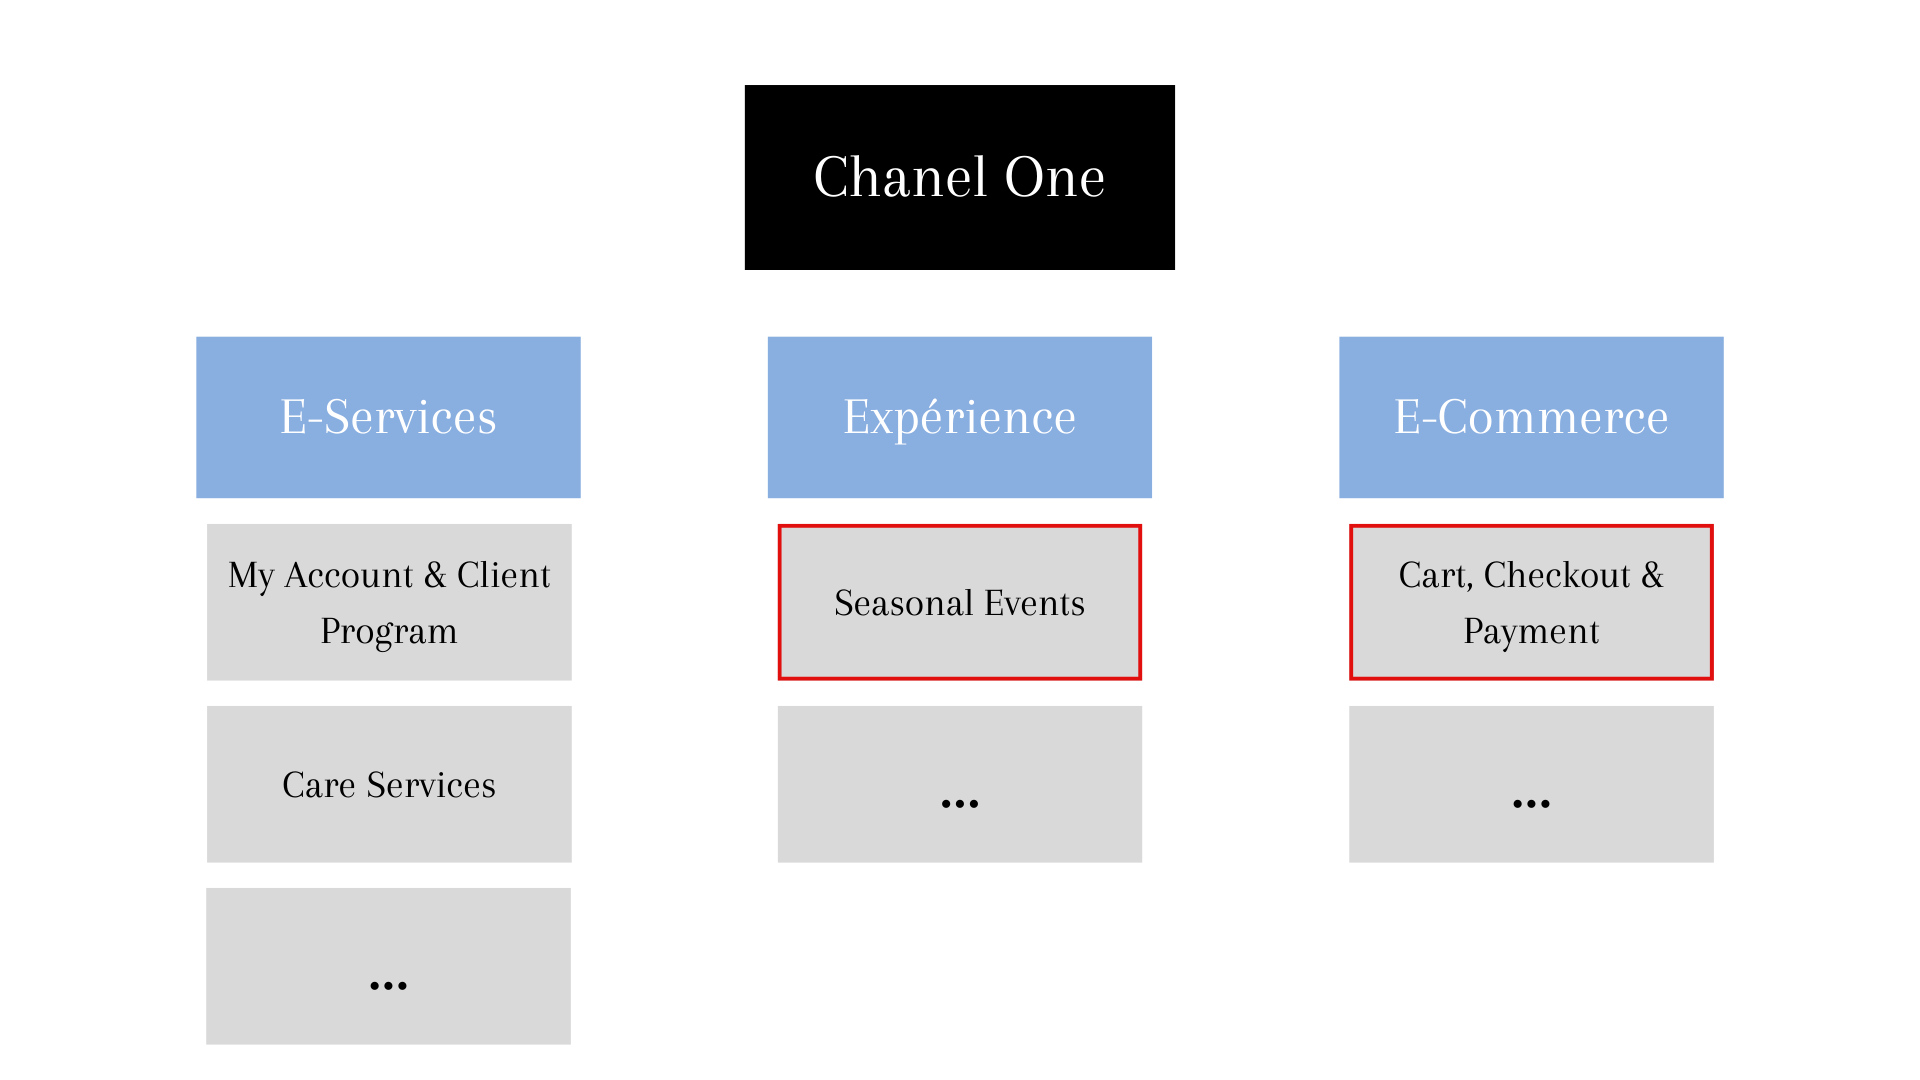
\includegraphics[width=19cm]{Figures/chanelOne.png}
    \captionof{figure}{Structure Chanel One}
    \label{fig:chanel}
\end{center}
\begin{itemize}
    \item \textbf{E-commerce :} Ce domaine englobe l'intégralité des processus liés à l'achat et à la gestion des commandes en ligne. Il couvre notamment la gestion des transactions, depuis l'ajout des produits au panier jusqu'à la finalisation du paiement. L'accent est mis sur l'intégration des méthodes de paiement sécurisées, comme Payconiq, tout en garantissant une fluidité optimale pour les clients. Il inclut également des services liés à la livraison, ainsi que la gestion des retours et des échanges, afin de fournir une expérience complète et sans friction, de l'achat à la réception des produits.
    \item \textbf{E-services :} Ce domaine se concentre sur les services numériques offerts pour enrichir l'expérience client. Cela comprend la gestion des comptes utilisateurs, permettant aux clients de suivre leurs commandes, de gérer leurs préférences et d'accéder aux programmes de fidélité. De plus, E-services inclut des fonctionnalités d'assistance après-vente, comme le suivi des réparations et des demandes spécifiques, et propose des outils permettant d'interagir avec les boutiques physiques, par exemple, en prenant rendez-vous ou en consultant la disponibilité des produits en magasin.
    \item \textbf{Expérience :} Ce domaine vise à améliorer en continu le parcours utilisateur. L'objectif est d'optimiser la présentation des produits et d'intégrer des fonctionnalités innovantes pour rendre la navigation sur le site plus intuitive et attractive. En combinant une esthétique raffinée et des outils techniques performants, le domaine Expérience garantit une interface utilisateur qui soit à la fois élégante et fonctionnelle.
\end{itemize}



\section*{Conclusion}
Au cours de ce chapitre, le périmètre du projet a été défini, ainsi que la méthodologie et le planning suivis pour sa réalisation. Le chapitre suivant abordera la phase d’analyse et de spécification du système à développer, visant à comprendre en profondeur les besoins des utilisateurs et à construire un système adapté à ces exigences.










\chapter{Analyse et spécification des besoins}
\label{chap:Analyse et spécification des besoins}

Ce chapitre présente l'analyse de l'existant et la spécification des besoins pour l'intégration de Bancontact by Payconiq. Nous examinerons les méthodes de paiement actuelles, les spécificités du marché belge, l'architecture existante, ainsi que les besoins fonctionnels et non fonctionnels.
\pagebreak

\section{Étude de l’existant}
\subsection{Méthodes de paiement actuelles}
Le site e-commerce de la marque propose actuellement une gamme diversifiée de méthodes de paiement reconnues mondialement, comprenant :
\begin{itemize}
    \item Visa
    \item MasterCard
    \item PayPal
    \item Klarna Pay Now
    \item Klarna Pay Later
    \item Chanel Gift Card
\end{itemize}
Bien que ces options répondent efficacement aux besoins d'une clientèle internationale, elles ne tiennent pas compte des spécificités locales de certains marchés clés, en particulier celui de la Belgique.
\subsection{Particularités du marché belge}
En Belgique, Bancontact s'est imposé comme l'une des méthodes de paiement privilégiées. Initialement conçu comme un système de paiement par carte de débit national, Bancontact est devenu un élément incontournable du paysage financier belge. Cette solution offre aux consommateurs belges la possibilité d'effectuer des paiements directs depuis leur compte bancaire, que ce soit en magasin, en ligne ou via une application mobile.
Face à l'évolution rapide des technologies et des attentes des consommateurs, Bancontact a réalisé une fusion stratégique avec Payconiq, une solution de paiement mobile innovante. Cette alliance a donné naissance à Bancontact by Payconiq, offrant aux utilisateurs belges une solution de paiement intégrée couvrant à la fois les transactions par carte et les paiements mobiles via une application dédiée.
L'adoption massive de cette solution en Belgique en fait un élément incontournable pour tout e-commerce aspirant à s'implanter solidement sur ce marché. Les chiffres parlent d'eux-mêmes : en 2023, près de 2 millions de Belges ont utilisé Payconiq pour leurs paiements mobiles, soulignant l'importance cruciale de cette méthode dans l'écosystème des paiements locaux.
\subsection{Justification de l'intégration de Bancontact by Payconiq}
L'intégration de Bancontact by Payconiq sur notre plateforme e-commerce présente plusieurs avantages stratégiques majeurs, particulièrement pour conquérir et fidéliser la clientèle belge :
\begin{itemize}
    \item [$\bullet$]\textbf{Adoption généralisée :} Avec une base d'environ 2 millions d'utilisateurs Payconiq et une forte pénétration de Bancontact dans les habitudes de paiement quotidiennes, cette solution est profondément ancrée dans le comportement des consommateurs belges.
    \item [$\bullet$]\textbf{Simplicité et ergonomie :} L'application "Payconiq by Bancontact" offre une expérience de paiement fluide et intuitive, reposant sur un simple scan de QR code, ce qui optimise considérablement le parcours client.
    \item [$\bullet$]\textbf{Sécurité renforcée :} La synergie entre les systèmes Bancontact et Payconiq garantit un niveau de sécurité optimal pour les transactions, s'appuyant sur des protocoles de sécurité robustes et éprouvés.
    \item [$\bullet$]\textbf{Interopérabilité bancaire :} Le support étendu de Payconiq par les principales institutions bancaires belges facilite son adoption et renforce la commodité pour les clients, en centralisant leurs opérations financières.
    \item [$\bullet$]\textbf{Essor des paiements mobiles :} Face à la croissance exponentielle des paiements mobiles en Belgique, l'intégration de solutions comme Payconiq s'avère cruciale pour capter et fidéliser une clientèle, particulièrement auprès des jeunes générations habituées aux transactions via smartphone.
\end{itemize}
\subsection{Architecture du processus de paiement actuel}
Le processus de paiement en place, présenté dans la figure \ref{fig:processus}, repose sur l'interaction harmonieuse de plusieurs systèmes interdépendants, chacun jouant un rôle déterminant dans la sécurisation des transactions et l'optimisation du traitement des commandes. 
\begin{center}
    \centering
    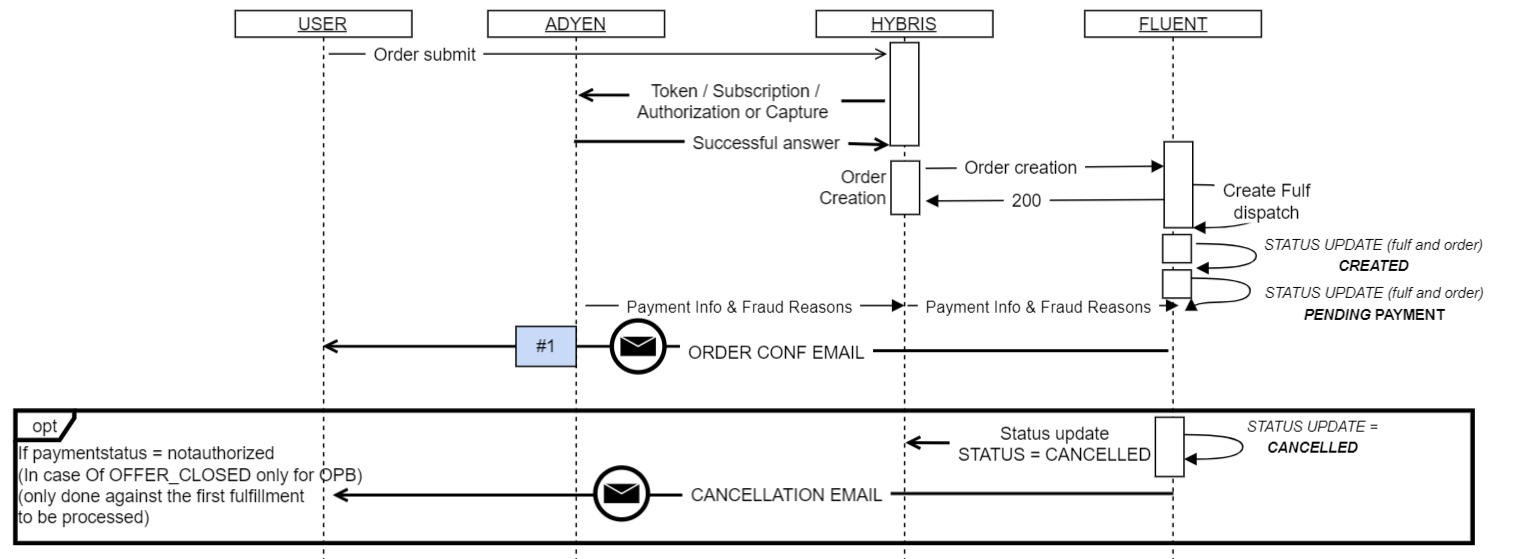
\includegraphics[width=19cm]{Figures/processus.jpeg}
    \captionof{figure}{Processus du paiement}
    \label{fig:processus}
\end{center}
Les composants clés du système sont les suivants :
\begin{itemize}
    \item [$\bullet$]\textbf{Hybris :} Plateforme e-commerce centrale, Hybris est responsable de la création des commandes une fois le paiement validé. Après la soumission d'une commande par l'utilisateur, Hybris communique avec Adyen pour le traitement du paiement. Une fois la confirmation reçue, Hybris crée officiellement la commande et notifie Fluent pour la gestion de l'expédition et du suivi.
    \item [$\bullet$]\textbf{Adyen :} En tant que fournisseur de services de paiement, Adyen gère la transaction financière. Il traite les détails du paiement transmis par Hybris, réalisant des actions telles que l'autorisation, la capture des fonds, ou la gestion des abonnements. Adyen joue un rôle clé dans la sécurisation et la validation des paiements avant la finalisation de la commande.
    \item [$\bullet$]\textbf{Fluent :} Système de gestion logistique, Fluent est responsable du cycle de vie de la commande après sa création dans Hybris. Il assure le suivi du processus de traitement, y compris la préparation de l'expédition, et met à jour les statuts de la commande (par exemple, "CREATED", "PENDING PAYMENT", "CANCELLED"). Fluent communique également avec Hybris pour informer les utilisateurs de l'état de leur commande.
\end{itemize}
Pour mieux comprendre le fonctionnement de ces composants, examinons le flux du processus de paiement étape par étape :
\begin{enumerate}
    \item \textbf{Initiation :} Le client valide son panier et soumet sa commande.
    \item \textbf{Transmission :} Hybris communique les informations de paiement à Adyen.
    \item \textbf{Traitement :} Adyen exécute la transaction et renvoie une confirmation à Hybris.
    \item \textbf{Création :} Hybris enregistre la commande et notifie Fluent pour la gestion logistique.
    \item \textbf{Suivi :} Fluent assure la gestion des statuts de commande et informe Hybris pour la mise à jour du client.
\end{enumerate}
\section{Etude fonctionnelle et non fonctionnelle}
Dans le cadre de l'intégration de Payconiq à la plateforme e-commerce du client, il est essentiel de définir clairement les besoins fonctionnels et non fonctionnels du projet. 
Cette étude permettra d'identifier les exigences spécifiques liées à cette intégration, assurant ainsi une mise en œuvre réussie et une expérience utilisateur optimale. 

\subsection{Exigences fonctionnelles}

\subsubsection{Identification des fonctionnalités}
\begin{itemize}
    \item [$\bullet$]\textbf{Sélection de Payconiq comme méthode de paiement :} L'option Payconiq doit être disponible lors de la finalisation de la commande, présentée de manière intuitive et clairement distinguée parmi les autres choix de paiement.
    \item [$\bullet$]\textbf{Génération et affichage du QR Code pour le paiement :} Lors de la confirmation de la commande avec Payconiq, un QR code unique est généré automatiquement et affiché à l'utilisateur pour permettre un paiement sécurisé via l'application Payconiq.
    \item [$\bullet$]\textbf{Suivi des transactions dans l'historique des commandes :} Les transactions effectuées avec Payconiq sont accessibles dans l'historique des commandes de l'utilisateur, avec une identification claire comprenant la date, le montant et l'état du paiement.
    \item [$\bullet$]\textbf{Envoi d'un email de confirmation de commande :} Après la finalisation de la commande, un email de confirmation est envoyé à l'utilisateur, incluant les détails de la commande, la méthode de paiement utilisée (Payconiq), le montant total et les informations de suivi de la commande.
    \item [$\bullet$]\textbf{Message d'erreur en cas d'échec du paiement :} En cas d'échec du paiement avec Payconiq, un message d'erreur explicite informe l'utilisateur du problème, avec des options de paiement alternatives proposées pour finaliser la transaction sans interruption.
\end{itemize}

\subsubsection{Diagramme de cas d’utilisation}


\subsubsection{Description textuelle de cas d’utilisation}


\subsubsection{Diagramme de séquence de système}

\subsection{Exigences non-fonctionnelles}

Les exigences non-fonctionnelles sont essentielles pour améliorer la qualité des services de la plateforme, notamment en termes de sécurité, de maintenabilité et de disponibilité. Elles garantissent non seulement une expérience utilisateur optimale, mais aussi la pérennité et l'efficacité du système face aux évolutions technologiques et aux besoins des utilisateurs. Parmi ces exigences, on peut citer :

\begin{itemize}
    \item [$\bullet$]\textbf{Sécurité :} La protection des informations sensibles des utilisateurs est cruciale dans tout système de paiement en ligne. L'intégration de Payconiq requiert une attention particulière à ces aspects pour éviter tout accès non autorisé et toute manipulation malveillante des données.
    \item [$\bullet$]\textbf{Maintenabilité :} La maintenabilité du système est essentielle pour garantir sa longévité et sa capacité à évoluer. Un code clair, bien structuré, et conforme aux meilleures pratiques de développement facilite l'ajout de nouvelles fonctionnalités et permet une correction rapide des bugs. Une bonne maintenabilité permet aux équipes de développement de diagnostiquer et de résoudre efficacement les problèmes, de déployer des mises à jour sans perturber le fonctionnement du système, et d'adapter rapidement le système aux évolutions technologiques et aux besoins des utilisateurs.
    \item [$\bullet$]\textbf{Disponibilité :} Le système doit être conçu pour faciliter le diagnostic, la résolution des problèmes, le déploiement des mises à jour, et l’adaptation aux évolutions technologiques et aux besoins des utilisateurs.
\end{itemize}


\section*{Conclusion}
La phase d'analyse de l'existant et de spécification des besoins est cruciale pour le succès de notre projet. Nous avons abordé cette phase en examinant l'architecture actuelle, en identifiant les acteurs clés et les cas d'utilisation spécifiques au marché belge. Ensuite nous avons entamé l'analyse des besoins fonctionnels et non fonctionnels. Dans les chapitres suivants, nous aborderons la conception détaillée du projet d'intégration.

\chapter{Conception de la solution}
\label{Conception de la solution}

Ce chapitre se concentre sur l'architecture physique et applicative adoptée. Il inclut également une exploration approfondie de la conception, illustrée par des diagrammes techniques de classes et de séquences détaillées, en se basant sur les spécifications établies dans le deuxième chapitre.
\newpage


\section{Architecture Globale}

L'architecture e-commerce, telle que présentée ici, est volontairement simplifiée pour se concentrer sur les composants essentiels sur lesquels nous avons travaillé. Elle s’appuie sur plusieurs composants clés pour gérer les interactions entre le client, le contenu du site, les commandes et les paiements.
\begin{center}
    \centering
    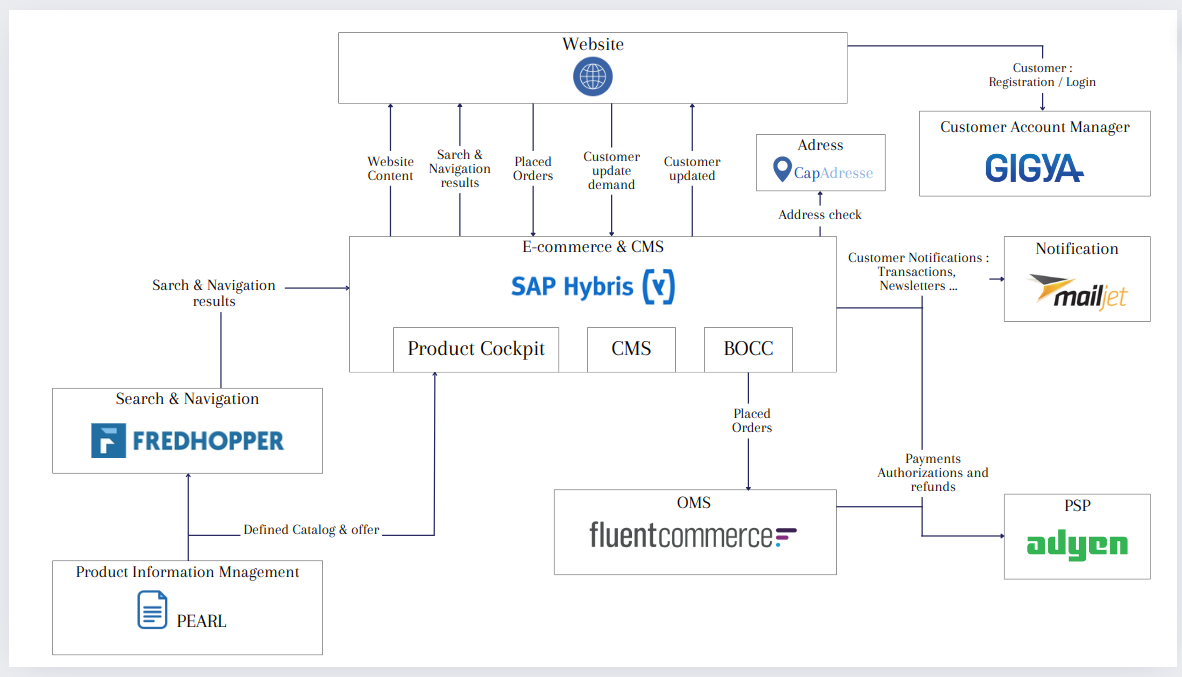
\includegraphics[width=19cm]{Figures/architectureGlobale.png}
    \captionof{figure}{Architecture globale de l'application E-commerce}
    \label{fig:processus}
\end{center}
\begin{itemize}
    \item [$\bullet$]Le site web permet aux clients de naviguer et de consulter le contenu (produits, offres, etc.). Le contenu est géré par le module CMS de SAP Hybris, qui centralise les informations et les affiches sur le storefront.
    \item [$\bullet$]Le moteur de recherche Fredhopper se charge de fournir les résultats de recherche et de navigation aux utilisateurs, en se basant sur les catalogues et les offres définis via PEARL, un système de gestion de l'information produit (PIM).
    \item [$\bullet$]Une fois la commande placée par le client via le site web, elle est prise en charge par SAP Hybris. Elle est ensuite transmise à Fluent Commerce, un système de gestion des commandes (OMS), qui suit et gère les différents statuts de la commande, depuis sa validation jusqu’à son expédition.
    \item [$\bullet$]CapAdresse est utilisé pour valider l’adresse du client avant la confirmation de la commande, afin de garantir la précision de la livraison.
    \item [$\bullet$]Mailjet est utilisé pour envoyer des notifications aux clients concernant les transactions, les newsletters, et d'autres communications, comme la confirmation de commande, d’expédition, ou d’annulation en cas de problème de paiement.
    \item [$\bullet$]Gigya s’occupe de la gestion des comptes clients, notamment l’enregistrement et la connexion des utilisateurs sur le site.
\end{itemize}
Lorsqu'un client effectue un paiement sur le site, une requête est envoyée à Adyen pour obtenir une autorisation. Adyen traite la demande et renvoie une réponse indiquant si le paiement est "autorisé" ou "non autorisé". Si le paiement est refusé, le client est redirigé vers une page d'erreur. En revanche, si le paiement est approuvé, le client est dirigé vers la page de confirmation de commande, et simultanément, la commande est exportée vers Fluent Commerce, le système de gestion des commandes.Fluent Commerce est chargé de gérer le cycle de vie de la commande en attendant la notification d'Adyen confirmant que le paiement a bien été autorisé, car il peut être annulé en cas de fraude ou de problème de sécurité. Si la notification indique que le paiement a été annulé, Fluent communique avec Mailjet pour envoyer un e-mail d'annulation au client. Cependant, si le paiement est confirmé, un e-mail de confirmation de commande est envoyé via Mailjet. Par la suite, une fois la commande prête à être expédiée, Fluent envoie une requête de capture à Adyen. Dès qu'Adyen confirme que la capture a été effectuée avec succès, la commande est expédiée, et Mailjet envoie un e-mail de confirmation de livraison au client. En plus de ces tâches, Fluent Commerce prend également en charge plusieurs aspects logistiques de la commande, tels que la vérification de la disponibilité des produits, la gestion des entrepôts pour l’expédition, ainsi que le suivi du statut de la commande (en attente, en préparation, expédiée, etc.).

\section{Architecture Backend}
Notre solution est basée sur la plate-forme SAP Hybris et suit donc son architecture
logicielle présentée dans la figure suivante :

\begin{center}
    \centering
    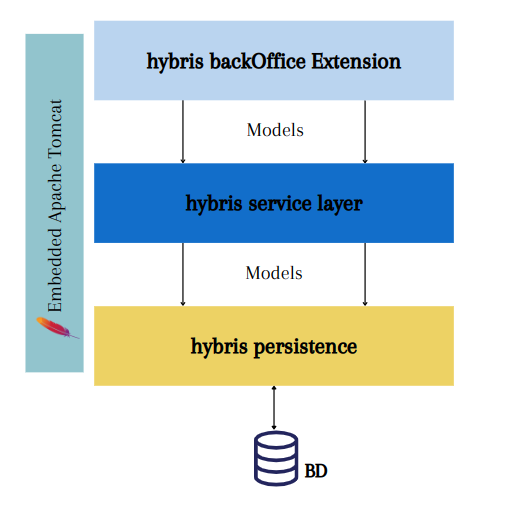
\includegraphics[width=19cm]{Figures/architecturebacend.png}
    \captionof{figure}{Architecture de backend de l'application E-commerce}
    \label{fig:processus}
\end{center}

\begin{itemize}
    \item [$\bullet$]\textbf{Serveur Apache Tomcat:} La plateforme Hybris utilise Apache Tomcat comme serveur HTTP intégré. Ce serveur d'application est responsable de l'hébergement de l'application Hybris et de la gestion des requêtes HTTP/HTTPS entrantes, assurant ainsi le bon fonctionnement de l'application web.
    \item [$\bullet$]\textbf{Extension Backoffice de Hybris:} L'extension Backoffice est une composante essentielle de Hybris qui permet aux utilisateurs métiers d'accéder aux fonctionnalités d'administration de contenu. Cela inclut la gestion du catalogue, des catégories, des produits, ainsi que des entités et types du système. Cette extension fournit une interface graphique conviviale pour les utilisateurs finaux, facilitant la gestion et l'organisation des données. En outre, elle offre aux développeurs la possibilité de créer ou de personnaliser des composants Hybris en fonction des besoins spécifiques de l'entreprise.
    \item [$\bullet$]\textbf{Service Layer de Hybris: }La couche de service (Service Layer) représente la couche métier de l'application Hybris, où est implémentée la logique de gestion d'entreprise. Elle est constituée d'un ensemble de services qui encapsulent les règles métiers et les processus de l'entreprise. La couche de service communique à la fois avec l'extension Backoffice et la couche de persistance via des modèles, qui sont des représentations des entités de la logique métier. Ces modèles servent d'intermédiaires entre les différentes couches, facilitant ainsi la manipulation des données de manière cohérente et sécurisée.
    \item [$\bullet$]\textbf{Couche de Persistance de Hybris:} La couche de persistance est le composant qui assure l'interaction entre le Service Layer et la base de données. Elle est responsable de la gestion de toutes les opérations de lecture et d'écriture dans la base de données, garantissant que les données sont stockées de manière efficace et peuvent être récupérées de manière fiable. 
\end{itemize}

\section{Environnent de livraison et test }


Cette section présente processus de déploiement du projet, en détaillant les différents serveurs utilisés. La structure se compose de deux parties principales : interne et externe.

\begin{center}
    \centering
    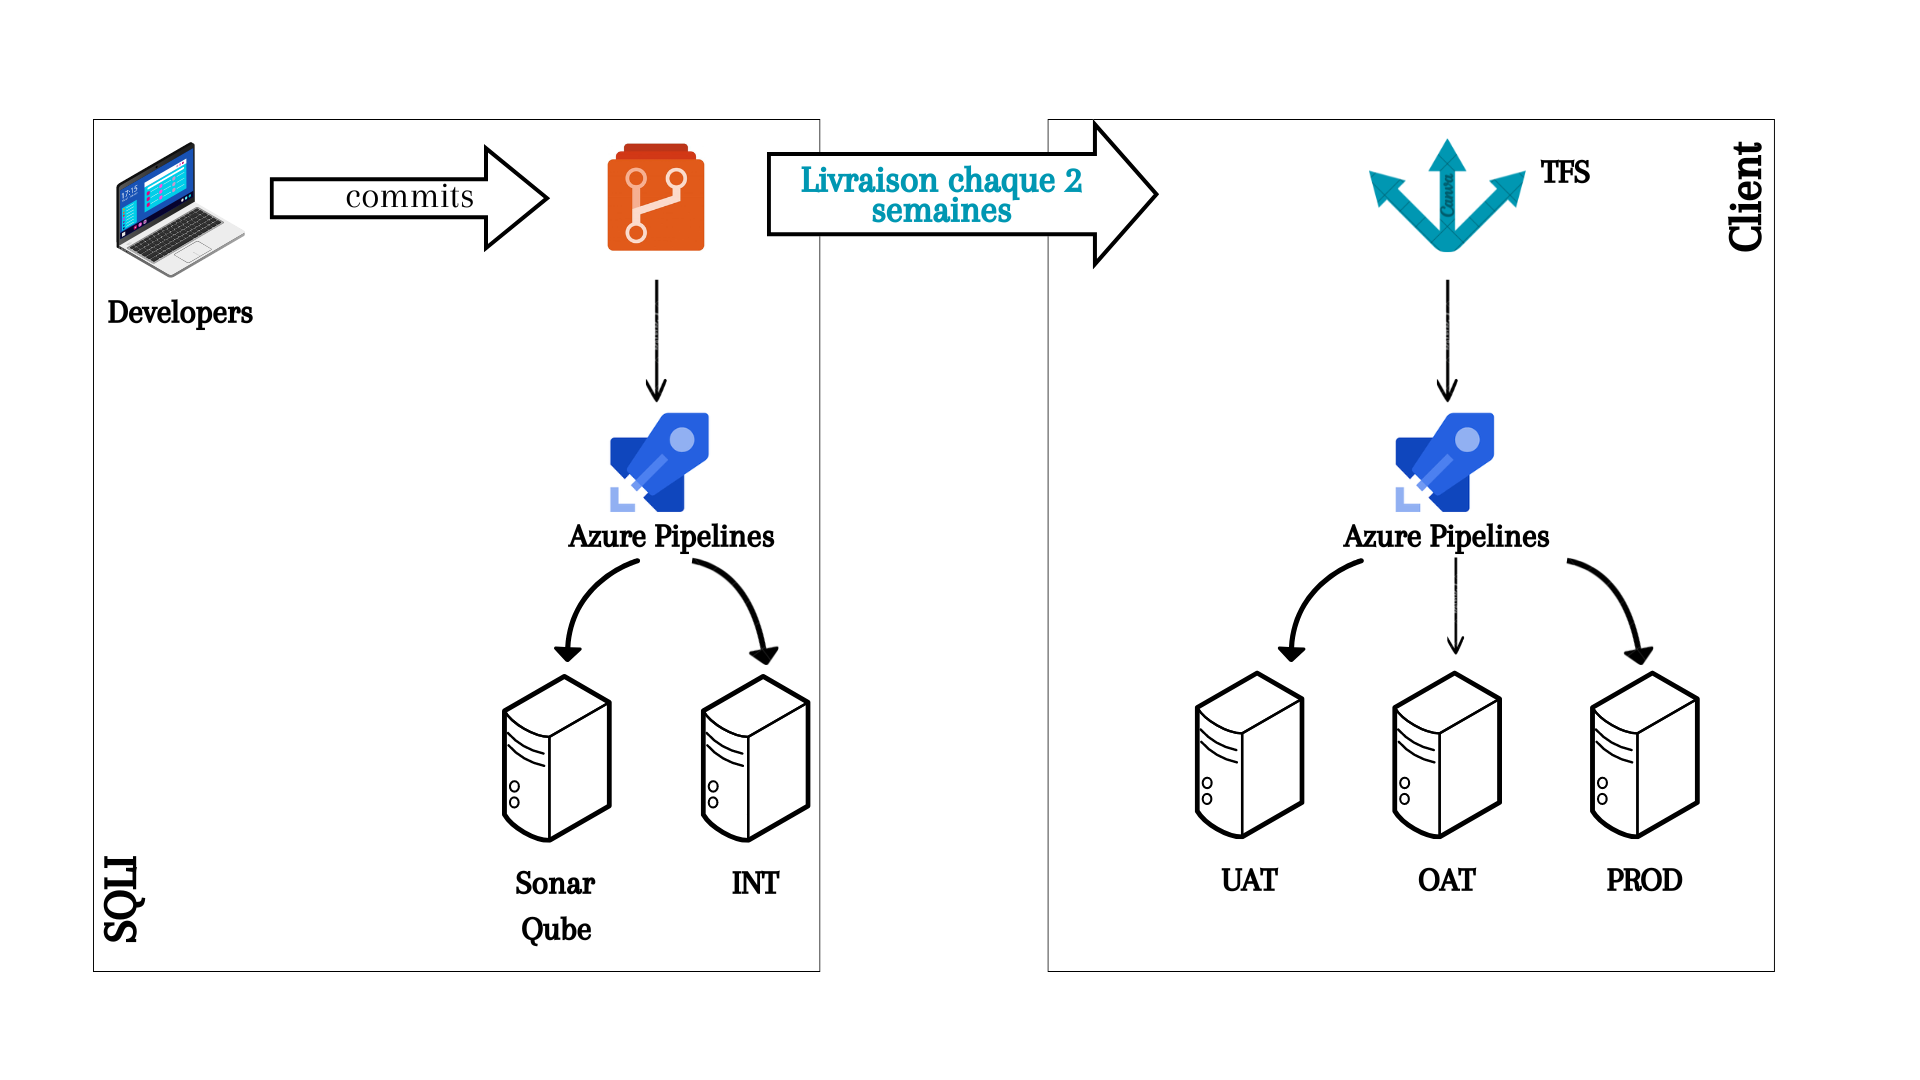
\includegraphics[width=19cm]{Figures/Test.png}
    \captionof{figure}{Architecture de livraison et test simplifiée}
    \label{fig:processus}
\end{center}
\begin{center}
    \centering
    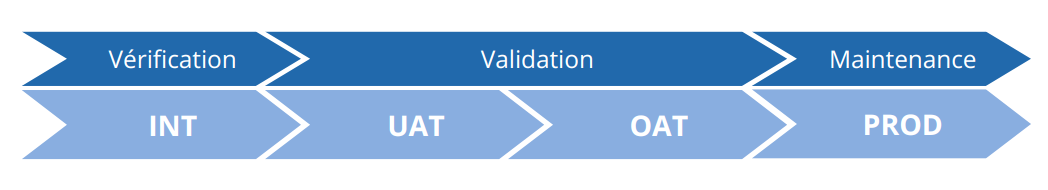
\includegraphics[width=19cm]{Figures/UAT.png}
    \captionof{figure}{Environnements de test et production}
    \label{fig:processus}
\end{center}



\subsection{Architecture interne}
L'architecture interne est implémentée au sein de SQLI et comprend un serveur d'intégration (INT) et un serveur SonarQube pour l'analyse de la qualité du code. Les développeurs effectuent des commits sur le dépôt Azure DevOps, puis un serveur d'intégration continue, Jenkins, récupère les dernières versions depuis ce dépôt pour effectuer une compilation automatique avec ANT. Jenkins lance ensuite une analyse SonarQube pour garantir la qualité du code. Après l'analyse SonarQube, le serveur vérifie que le nombre d'erreurs détectées ne dépasse pas les limites prédéfinies en fonction de la gravité des erreurs et des quotas définis sur le serveur SonarQube. Si ces contrôles sont satisfaits, Jenkins déploie le code sur le serveur d'intégration (INT). Ce processus d'intégration continue se répète tout au long du sprint de trois semaines.


\subsection{Architecture externe}

L'architecture externe est implémentée dans l'environnement du client et se compose de trois serveurs : UAT (User Acceptance Testing), OAT (Operational Acceptance Testing) et PROD (Production). Toutes les deux semaines, une nouvelle version est livrée dans le système de gestion de versions du client, TFS (Team Foundation Server).

\begin{itemize} \item [$\bullet$]\textbf{Serveur UAT:} Utilisé pour tester les livrables et s'assurer qu'ils répondent aux attentes de l'utilisateur final. \item [$\bullet$]\textbf{Serveur OAT:} Permet de déterminer si les livrables sont opérationnels et prêts à être intégrés dans l'environnement de production. \item [$\bullet$]\textbf{Serveur PROD:} Après les processus de test, une mise en production (MEP) est effectuée tous les trois mois, rendant la version finale disponible pour les utilisateurs finaux. \end{itemize}

\section{Architecture applicative}

Dans le cadre de l'utilisation de la solution Hybris, il est conseillé de suivre l'architecture applicative qu'elle propose. Cette architecture est basée sur un modèle n-tiers largement utilisé dans les applications web, permettant une répartition claire des rôles et une meilleure structuration du code. Quatre principaux patrons de conception sont au cœur de cette architecture :

\begin{center}
    \centering
    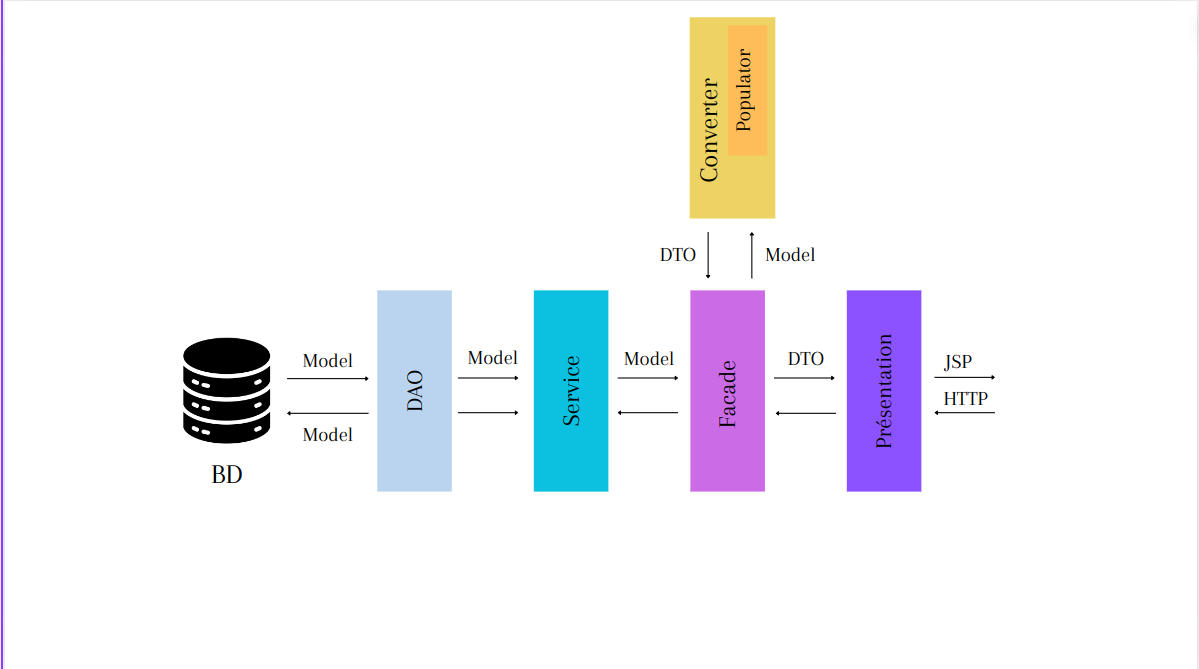
\includegraphics[width=19cm]{Figures/Dto.png}
    \captionof{figure}{Architecture Applicative de l'application E-commerce}
    \label{fig:processus}
\end{center} 

\begin{itemize}
    \item[$\bullet$] \textbf{Modèle MVC (Modèle-Vue-Contrôleur)} : Ce modèle permet de séparer distinctement la présentation, la logique métier et l'accès aux données. Cela garantit une organisation modulaire, rendant l'application plus facile à maintenir et à étendre. Par exemple, dans notre application, la vue pourrait être gérée par des pages JSP ou des composants front-end, tandis que les contrôleurs orchestrent les opérations de la logique métier encapsulée dans les services.

    \item[$\bullet$] \textbf{Patron de Façade} : Ce patron vise à simplifier l'accès à un système complexe en fournissant une interface unique et uniforme. Il permet d'interagir facilement avec des sous-systèmes tout en masquant leur complexité interne. Dans notre projet, une façade serait utile pour centraliser les interactions entre les services et les DAO, en facilitant ainsi l'appel des contrôleurs.

    \item[$\bullet$] \textbf{Patron DAO (Data Access Object)} : Ce patron permet d'accéder aux données sans être lié à un SGBD spécifique, en fournissant une abstraction qui rend l'application plus flexible. Il encapsule la logique d'accès aux données, permettant d'intégrer facilement différents SGBD sans modifier le code de l'application. Par exemple, le DAO pour "Produit" ou "Client" peut contenir toute la logique nécessaire pour interagir avec les données associées, indépendamment de la base utilisée.

    \item[$\bullet$] \textbf{Patron DTO (Data Transfer Object)} : Ce modèle optimise les échanges de données entre différentes couches de l'application en regroupant les informations dans des objets spécifiques. Il permet de réduire la surcharge de transfert de données, améliorant ainsi l'efficacité des communications entre les couches. Dans notre application, les DTO servent de pont entre la couche de service et la présentation, réduisant les dépendances et simplifiant les tests unitaires.
\end{itemize}

Adopter cette architecture permet non seulement une meilleure organisation du code, mais aussi d'assurer une évolutivité et une maintenance aisée à long terme.

\section{Diagramme de classe}
\begin{center}
    \centering
    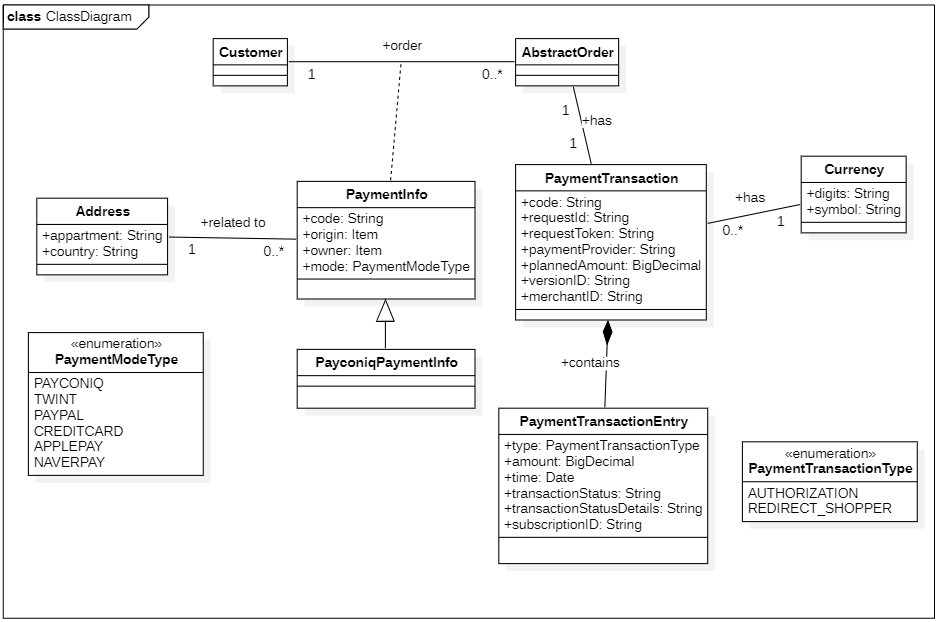
\includegraphics[width=19cm]{Figures/class.png}
    \captionof{figure}{Diagramme de classe}
\end{center}

La figure ci-dessus représente le diagramme de classe de notre système. Un Client peut passer plusieurs Commandes (représentées par la classe AbstractOrder), et chaque commande est associée à une Transaction de paiement (PaymentTransaction). Cette transaction contient des détails tels que le fournisseur de paiement, le montant prévu, et les identifiants du marchand. Elle est liée à une ou plusieurs Entrées de transaction (PaymentTransactionEntry), qui décrivent des aspects spécifiques comme le type de transaction, le montant, l'heure, et l'état de la transaction. Les informations de paiement sont représentées par la classe PaymentInfo, qui inclut le mode de paiement (défini par l'énumération PaymentModeType), et peut être associée à une Adresse. Une spécialisation de PaymentInfo, nommée PayconiqPaymentInfo, est utilisée pour les transactions via Payconiq. Le système gère également les devises via la classe Currency, qui est associée aux transactions de paiement. En somme, ce diagramme modélise la partie structurelle d'un volet de la gestion de paiement dans notre site e-commerce où les clients effectuent des paiements par divers moyens.

\section{Diagramme de séquence}

\begin{center}
    \centering
    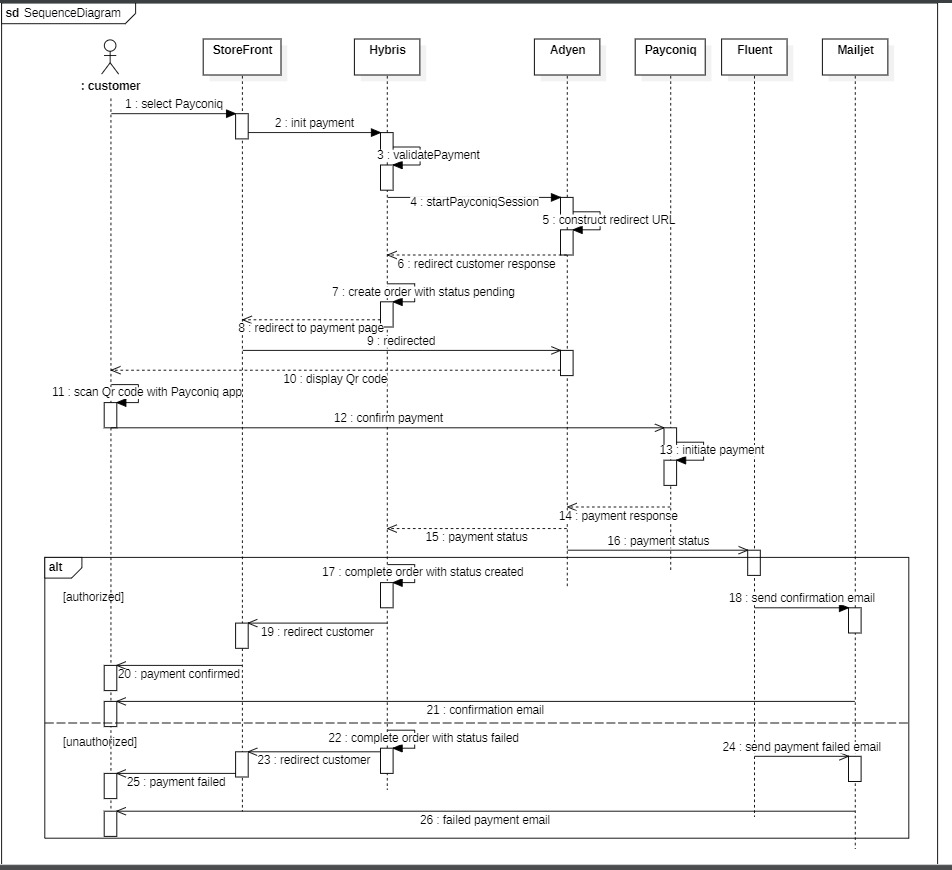
\includegraphics[width=19cm]{Figures/sequence.png}
    \captionof{figure}{Diagramme de séquence }
    \label{fig:processus}
\end{center} 


Le processus de paiement via Payconiq commence lorsque le client sélectionne ce moyen de paiement sur la plateforme. La transaction est alors initialisée et validée pour s'assurer que toutes les conditions sont remplies. Ensuite, une session Payconiq est démarrée via Adyen, qui génère une URL de redirection pour amener le client à la page de paiement Payconiq. Une fois redirigé, une commande est créée avec le statut "en attente". La page de paiement affiche un QR code que le client doit scanner avec son application Payconiq. Après avoir scanné le QR code, la confirmation du paiement est envoyée de Payconiq à Adyen, qui informe ensuite la plateforme e-commerce du statut du paiement.

Si le paiement est autorisé, la commande est complétée avec le statut "créée", le client est redirigé vers une page de confirmation, et un e-mail de confirmation de commande est envoyé. En revanche, si le paiement échoue, la commande est marquée avec le statut "échec", le client est redirigé vers une page d'échec de paiement, et un e-mail d'échec de paiement est envoyé.



\subsection*{Conclusion}

Ce chapitre a été dédié à l’étude conceptuelle du projet. Après une présentation des architectures adoptées et des divers diagrammes techniques de classes et de séquences, une compréhension approfondie du projet a été acquise. La prochaine étape consistera à aborder l’implémentation et la validation de la solution, sujet du chapitre suivant.
\pagebreak

\chapter{Implémentation et Validation}
\label{chap:Implémentation et Validation}


Ce chapitre décrit l'implémentation du travail réalisé. Il commence par une présentation des technologies utilisées, suivie de captures d'écran illustrant les différentes fonctionnalités développées. Ensuite, les tests effectués sont exposés.
\newpage
\section{Technologies utilisées}
\subsection*{$\bullet$ SAP Commerce (Hybris)}
\begin{center}
    \centering
    
\includegraphics[scale=0.5]{Figures/SAP.jpg}
    \captionof{figure}{Logo de SAP }
    \label{fig:processus}
\end{center} 

SAP Commerce (Hybris) est une plateforme de commerce électronique robuste et évolutive, conçue pour gérer efficacement les catalogues de produits, les commandes, les paiements, ainsi que les interactions avec les clients à travers divers canaux tels que le web, les appareils mobiles, et les points de vente physiques. Dans le cadre de ce projet, SAP Commerce a été choisi pour sa capacité à intégrer des outils de suivi des performances et de marketing, offrant ainsi une gestion complète du commerce en ligne et une expérience utilisateur optimale.

\subsection*{$\bullet$ JEE (JSP)}
\begin{center}
    \centering
    
\includegraphics[scale=0.5]{Figures/jee.png}
    \captionof{figure}{Logo de JEE}
    \label{fig:processus}
\end{center} 

JEE (JSP) a été utilisé pour développer la partie frontend de la méthode de paiement. En combinant du code Java et HTML, JSP facilite la création de pages web dynamiques permettant l'affichage interactif des informations de paiement et la gestion des transactions utilisateur. Cette technologie a permis de concevoir une interface utilisateur réactive tout en tirant parti de la flexibilité et de la puissance du backend Java pour assurer une gestion efficace des flux de paiement.
\subsection*{$\bullet$ Spring}
\begin{center}
    \centering
    
\includegraphics[scale=0.4]{Figures/spring.png}
    \captionof{figure}{Logo de Spring}
    \label{fig:processus}
\end{center} 

Spring a été employé pour développer la logique métier associée à la nouvelle méthode de paiement. Il a permis la création de services back-end pour la validation des paiements, l'interaction avec les systèmes de paiement externes, et le traitement des retours d'information. Grâce à son intégration transparente avec SAP Commerce (Hybris), Spring a assuré une séparation claire des responsabilités et une maintenabilité accrue du code, tout en exploitant ses fonctionnalités avancées pour la gestion des transactions et la sécurité.
\subsection*{$\bullet$ SonarQube}
 \begin{center}
    \centering
    
\includegraphics[scale=0.15]{Figures/sonarqube.png}
    \captionof{figure}{Logo de SonarQube}
    \label{fig:processus}
\end{center} 

SonarQube est un outil d'analyse statique de code permettant de détecter les bugs, les vulnérabilités de sécurité, et d'évaluer la qualité du code source. Dans ce projet, SonarQube a été utilisé pour analyser le code existant et les nouvelles fonctionnalités ajoutées. L'outil a permis de corriger les bugs et les failles de sécurité identifiés, tout en fournissant des recommandations pour améliorer la structure et la lisibilité du code, garantissant ainsi le respect des standards de qualité requis par le client.
\subsection*{$\bullet$ Ant}
\begin{center}
    \centering
    
\includegraphics[scale=0.05]{Figures/Ant.png}
    \captionof{figure}{Logo d'Ant}
\end{center}

Ant est un outil de build open-source qui permet d'automatiser diverses tâches liées au processus de développement, telles que la compilation, le déploiement, et l'exécution des tests. Dans le cadre de ce projet, Ant a été utilisé pour automatiser la compilation du code, faciliter le débogage, et exécuter les tests unitaires. Grâce à sa configuration native avec Hybris, qui utilise des scripts Ant prédéfinis, Ant a contribué à une organisation efficace des étapes de développement, assurant ainsi un flux de travail structuré et fluide.
\subsection*{$\bullet$ JUnit}
\begin{center}
    \centering
    
\includegraphics[scale=0.5]{Figures/junit.png}
    \captionof{figure}{Logo de JUnit}
    \label{fig:processus}
\end{center}

JUnit est un framework de tests unitaires en Java utilisé pour tester les composants individuels d'une application. Pour l'intégration de la nouvelle méthode de paiement, JUnit a été employé pour écrire des tests unitaires afin de vérifier la fiabilité des fonctionnalités back-end. Les tests couvraient divers scénarios, y compris la validation des transactions, la gestion des erreurs, et les interactions avec les systèmes externes.
\section{Illustration de l'Intégration de la Méthode de Paiement}
Cette partie fournit une vue détaillée des fonctionnalités développées à travers une série de captures d’écran.
Avant de finaliser l'intégration de Payconiq via Adyen, il est crucial de vérifier que cette méthode de paiement est correctement activée dans le système. Comme le montre la figure \ref{fig:activ}, Payconiq est marqué comme actif dans le Cockpit d'administration de SAP Commerce. 
Cela confirme qu'il est prêt à être utilisé pour le traitement des paiements, garantissant que les transactions effectuées avec Payconiq seront traitées correctement.
\begin{center}
    \centering
    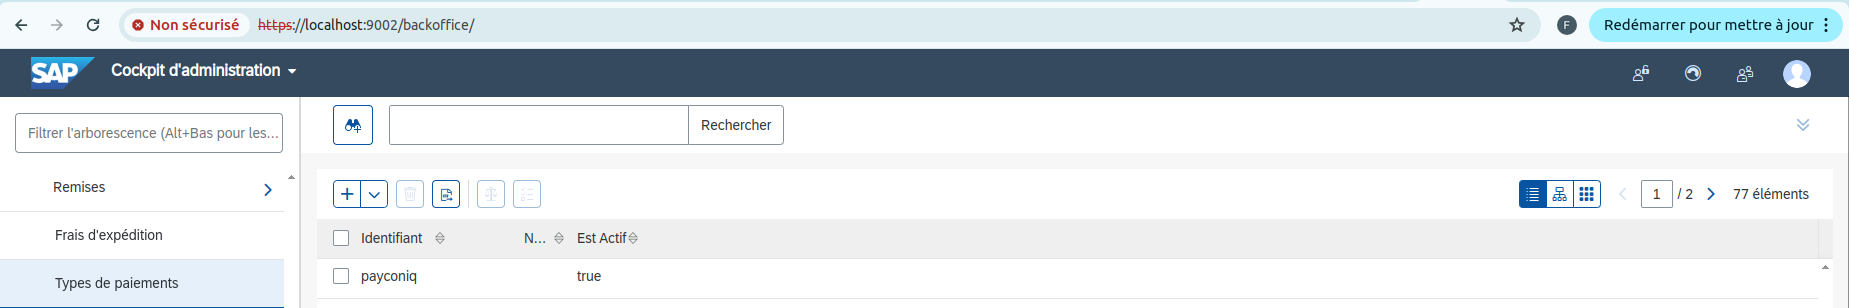
\includegraphics[width=19cm]{Figures/Screens/VERIFIER QUE payment activer.png}
    \captionof{figure}{Activation de Payconiq}
    \label{fig:activ}
\end{center}

Une fois activée, Payconiq a été ajoutée à la boutique en ligne pour le marché belge. La figure \ref{fig:disp} montre que Payconiq apparaît désormais parmi les méthodes de paiement disponibles dans l'onglet eCommerce, aux côtés de giftcard, applepay-eu, et paypal-eu. Cette configuration permet aux utilisateurs de choisir Payconiq lors de la validation de leur commande.
\begin{center}
    \centering
    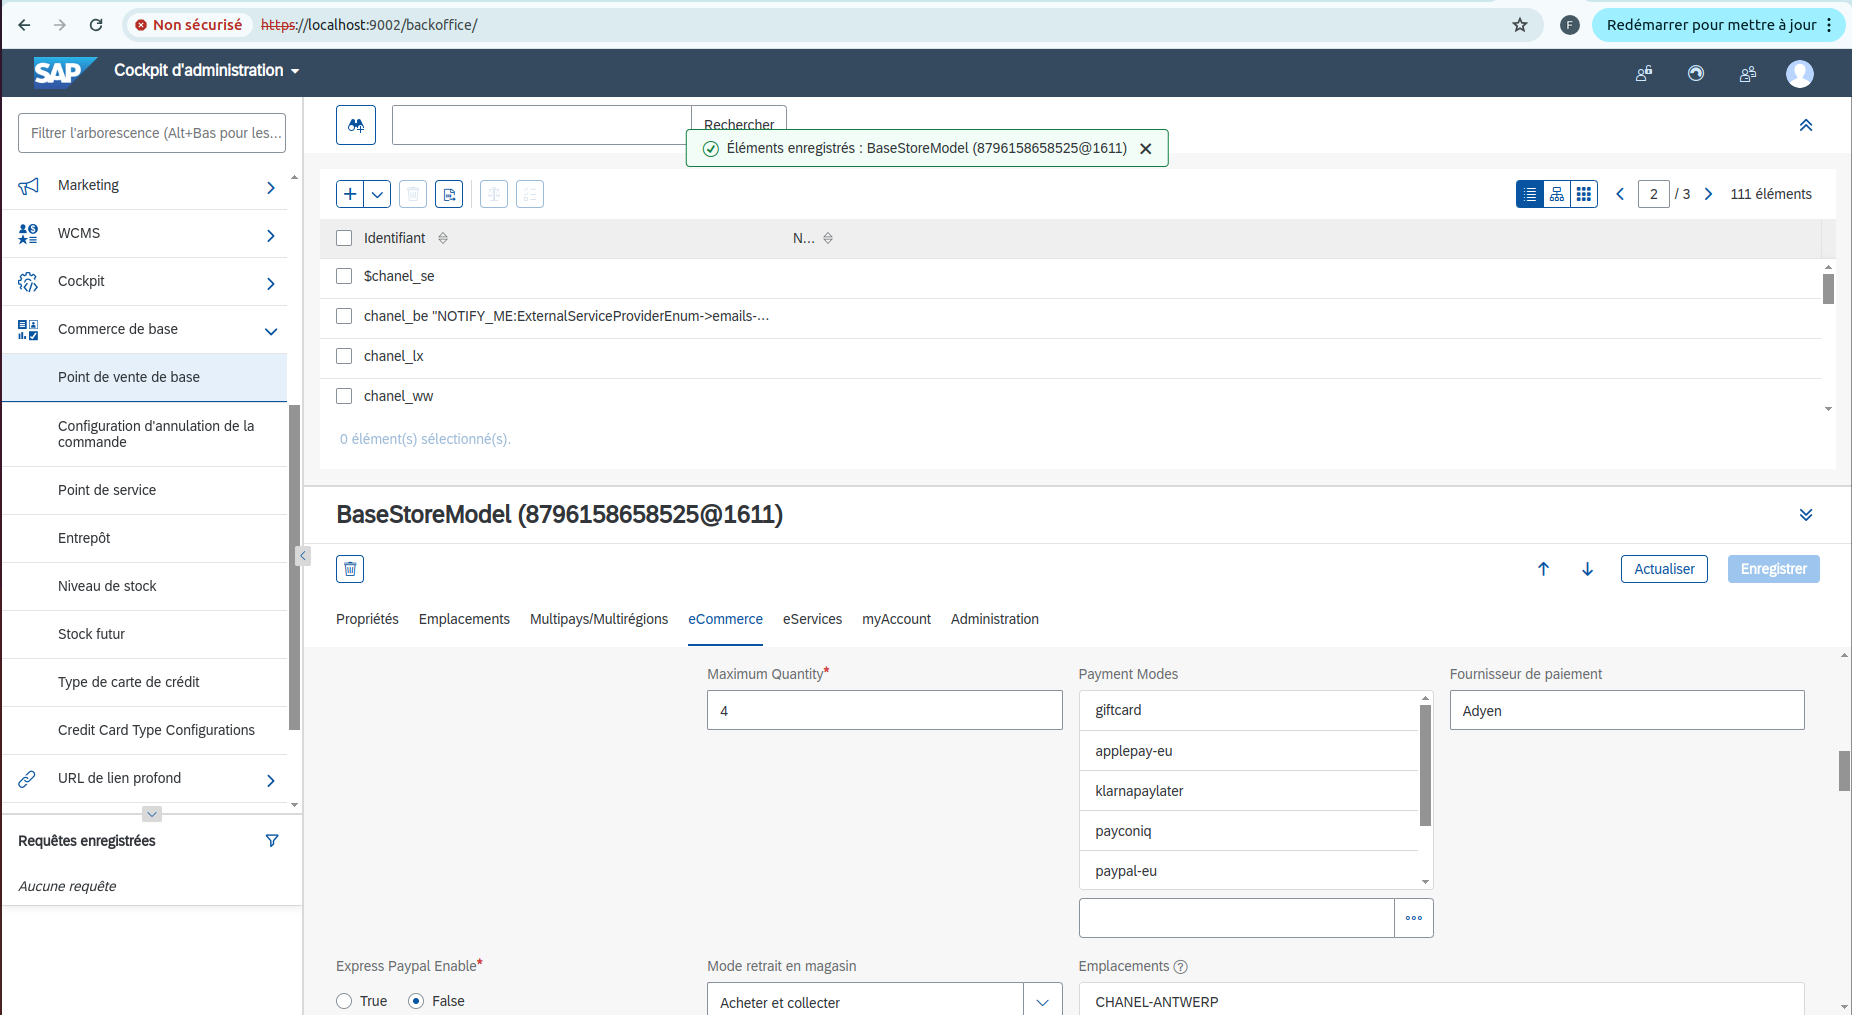
\includegraphics[width=19cm]{Figures/Screens/activation du payconiq pour belge.png}
    \captionof{figure}{Disponibilité de Payconiq dans la boutique en ligne}
    \label{fig:disp}
\end{center}
Lorsque le client sélectionne les articles désirés, il passe à la phase de paiement. La figure \ref{fig:selection} illustre l'ajout d'un produit au panier, une étape préalable au paiement.
\begin{center}
    \centering
    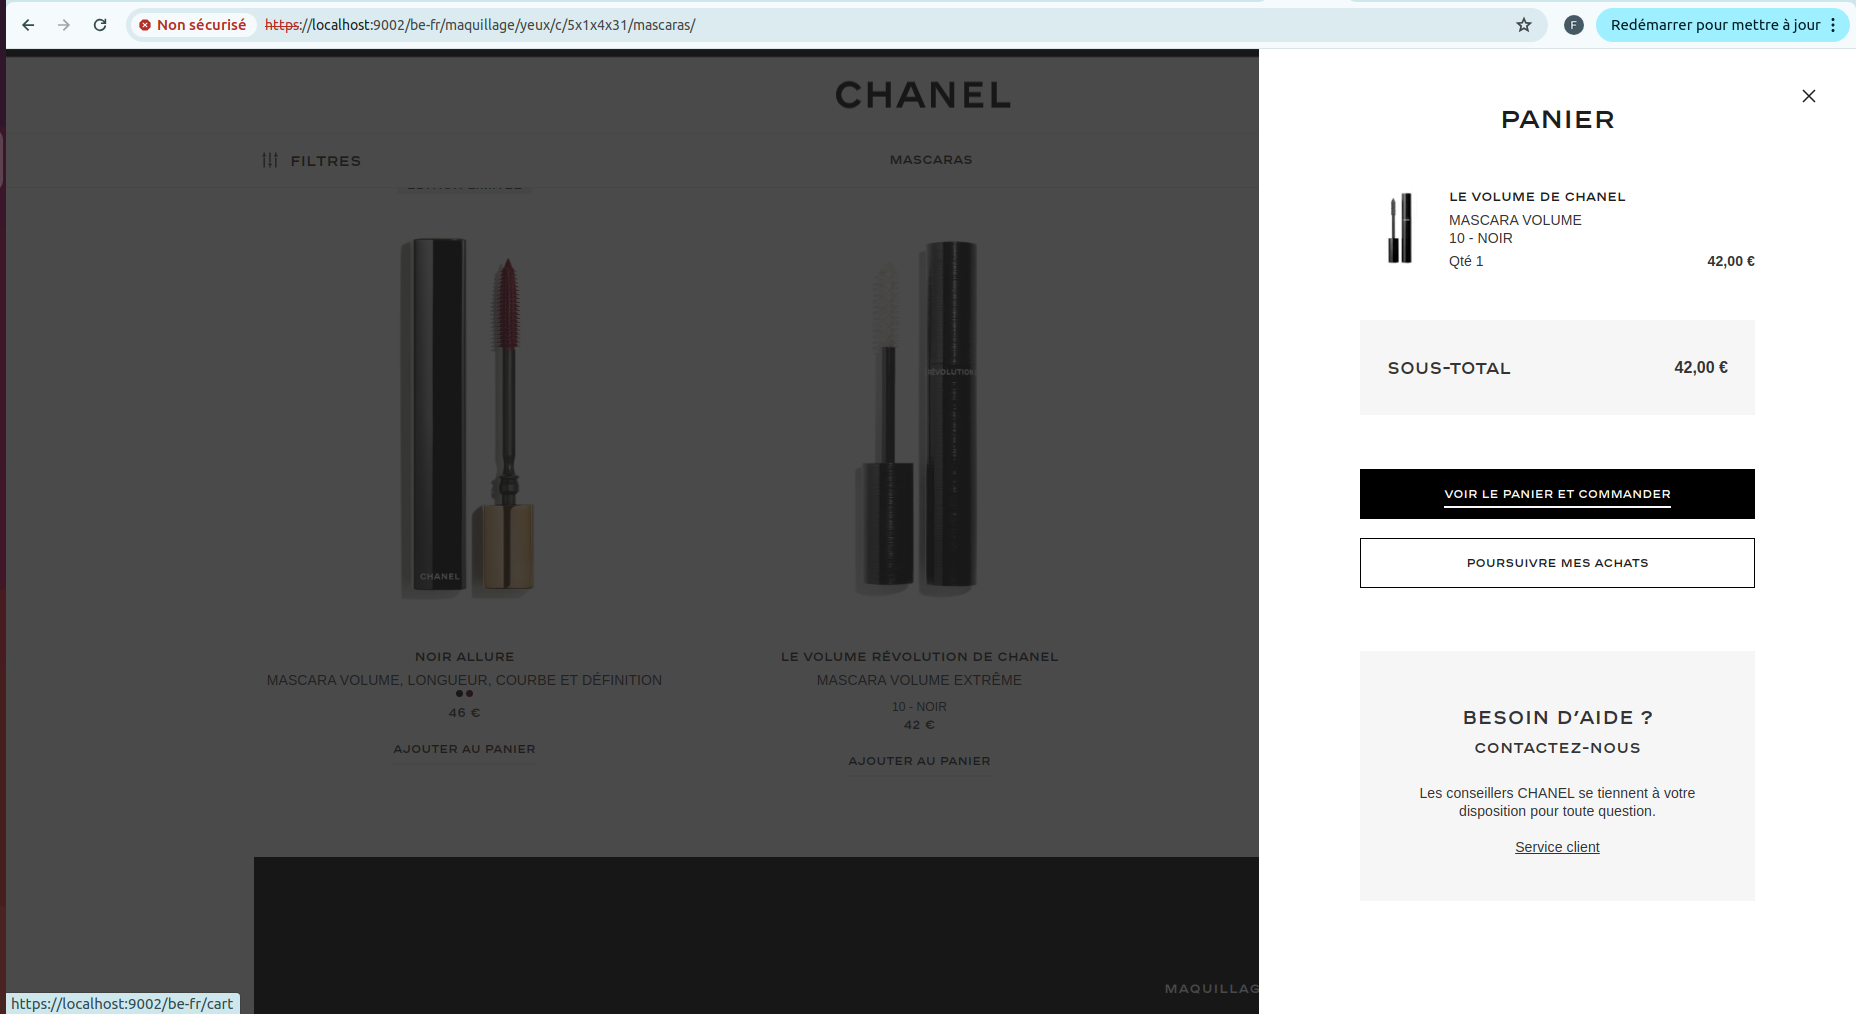
\includegraphics[width=19cm]{Figures/Screens/ajouter un produit au panier.png}
    \captionof{figure}{Ajout d'un produit au panier}
    \label{fig:selection}
\end{center}
C'est ici que commence la première étape du processus de paiement, où l'utilisateur est invité à saisir ses informations personnelles, y compris l'adresse e-mail, comme le montre la figure \ref{fig:saisie}.
\begin{center}
    \centering
    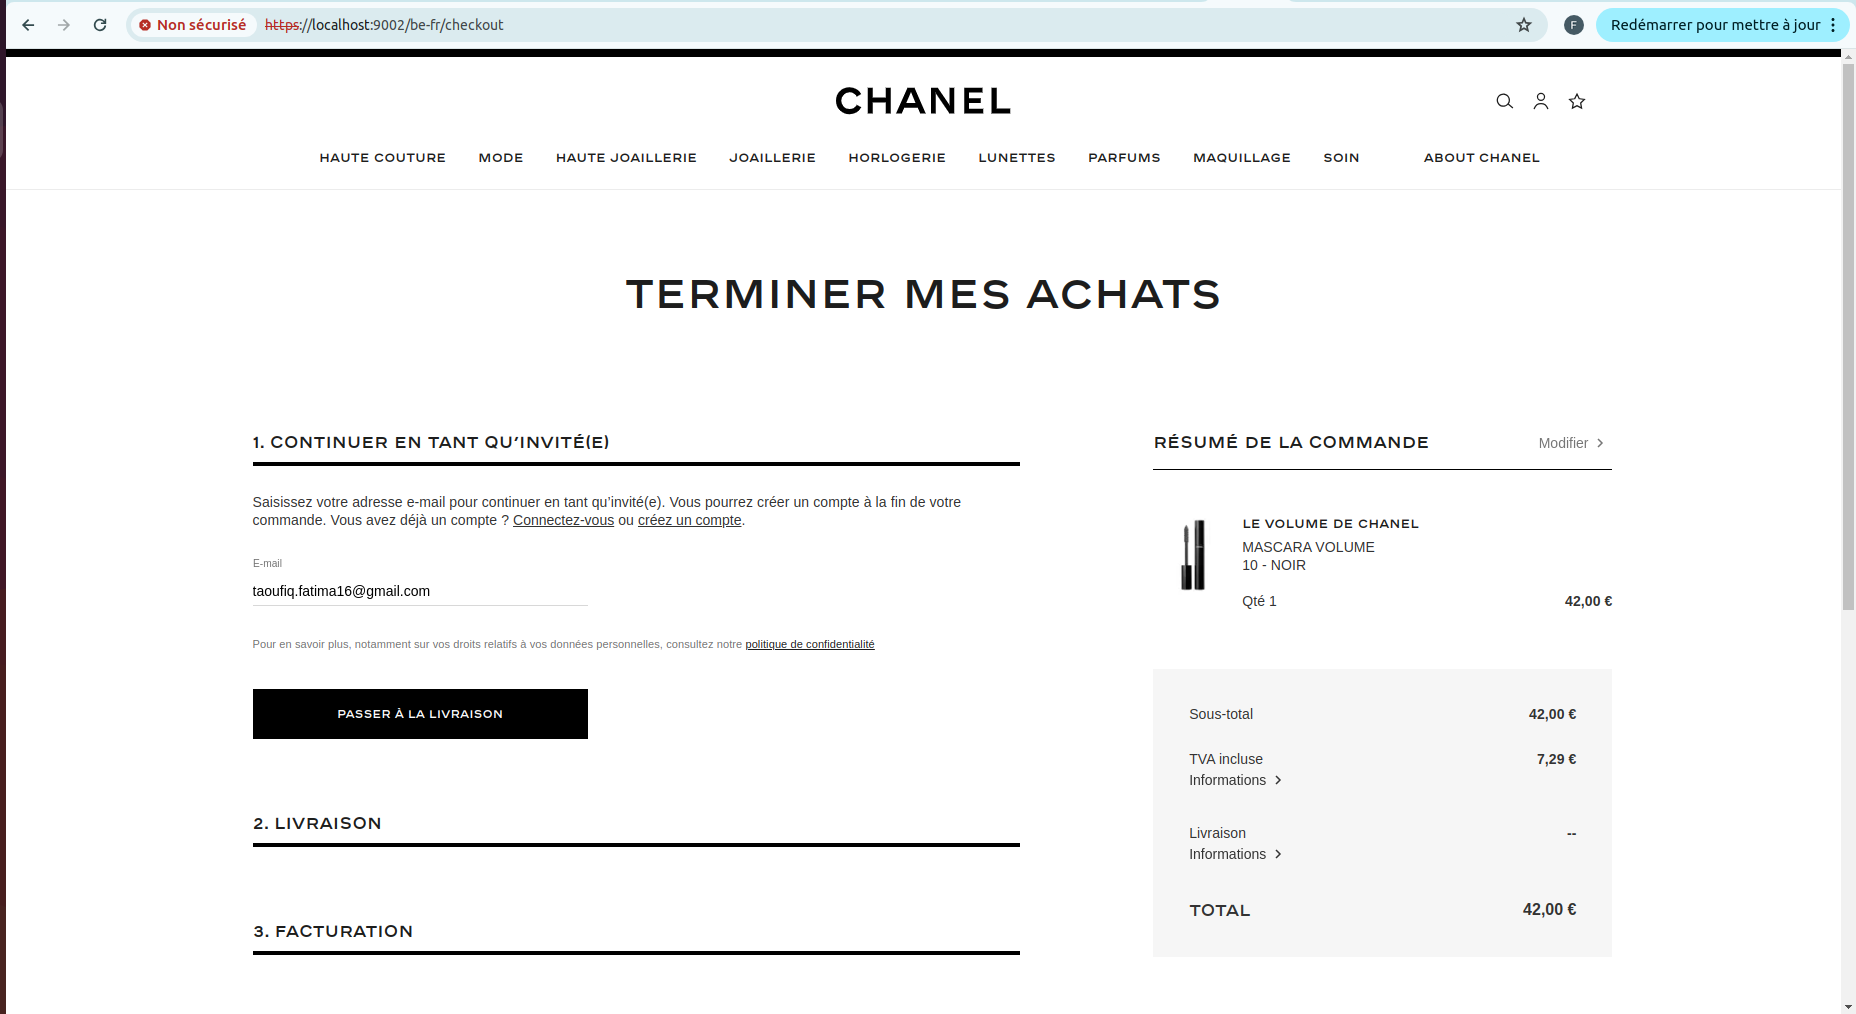
\includegraphics[width=19cm]{Figures/Screens/ajout de l'email.png}
    \captionof{figure}{Saisir les informations personnelles}
    \label{fig:saisie}
\end{center}
Après avoir rempli ses informations personnelles, l'utilisateur passe à la deuxième étape du processus de paiement, dédiée à la sélection du mode de livraison. Comme illustré dans la figure \ref{fig:mode}, cette étape permet à l'utilisateur de choisir entre la livraison à domicile ou le retrait en magasin (Click \& Collect). 
En fonction de l'option sélectionnée, l'interface offre les champs nécessaires : pour la livraison à domicile, l'utilisateur doit Saisir une adresse complète, tandis que pour le retrait en magasin, il choisit le point de retrait souhaité. Cette personnalisation assure une expérience de commande adaptée aux préférences de livraison de chaque utilisateur.
\begin{center}
    \centering
    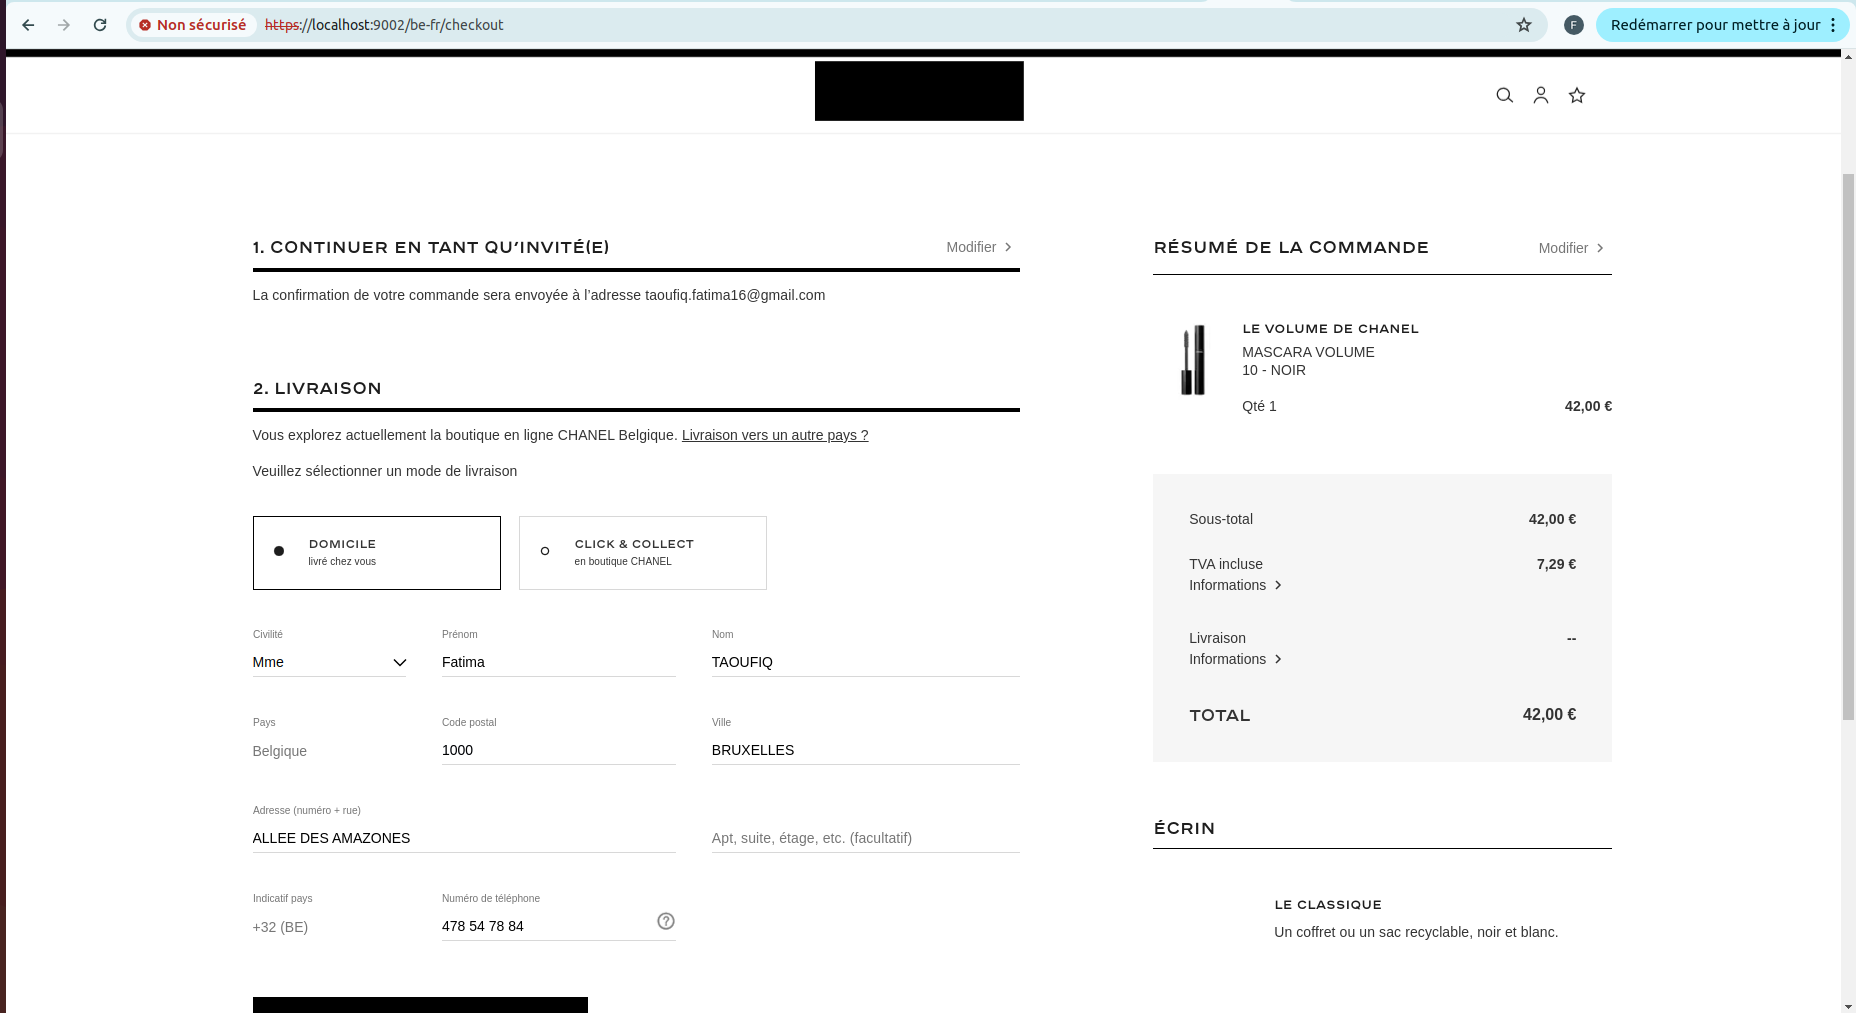
\includegraphics[width=19cm]{Figures/Screens/Infos livraison.png}
    \captionof{figure}{Mode de livraison}
    \label{fig:mode}
\end{center}
Si un code promotionnel est disponible, l'utilisateur peut l'entrer dans le champ prévu à cet effet (\textit{Figure \ref{fig:promo}}) pour bénéficier d'une réduction. 
\begin{center}
    \centering
    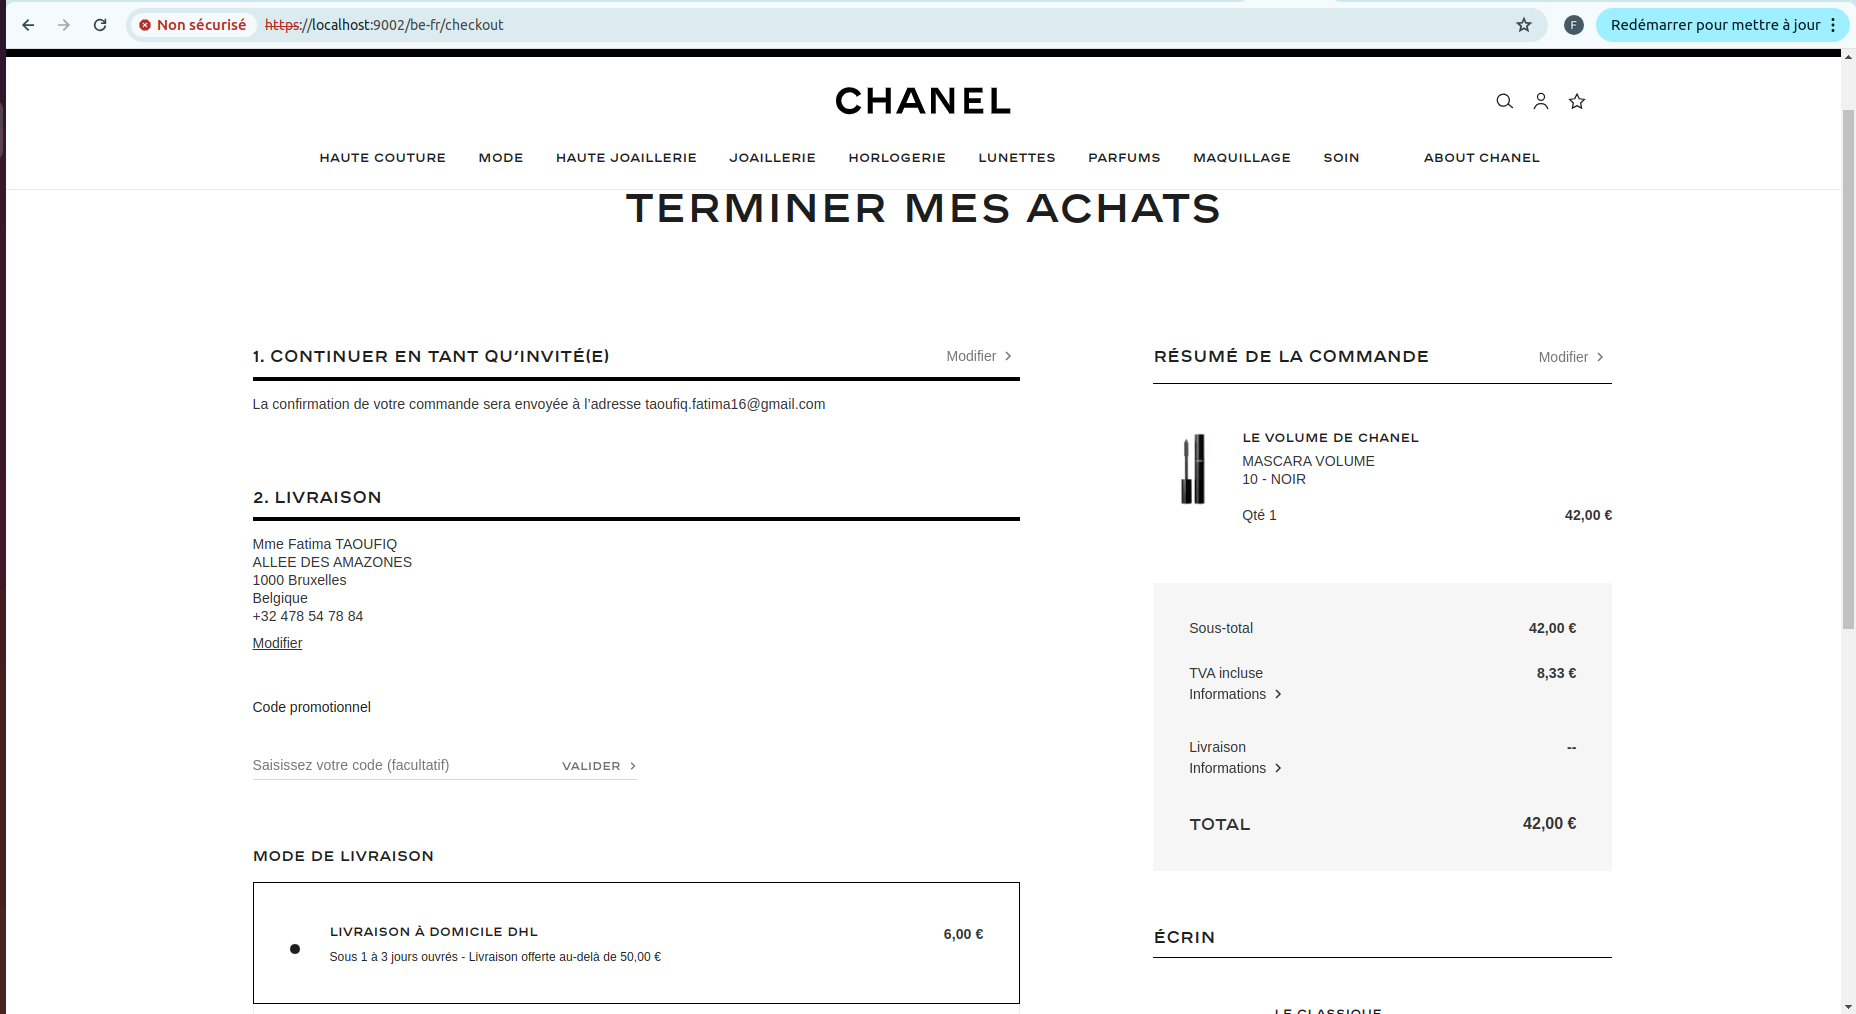
\includegraphics[width=19cm]{Figures/Screens/code prommo.png}
    \captionof{figure}{Saisir un code promo}
    \label{fig:promo}
\end{center}
En l'absence de code, l'utilisateur poursuit directement vers l'étape suivante : la facturation. À ce stade, il est invité à saisir ses informations de facturation. L'interface (\textit{Figure \ref{fig:facturation}}) propose de reprendre automatiquement l'adresse de livraison pour simplifier le processus, mais permet également de renseigner une adresse différente si nécessaire. Cette flexibilité assure que les informations de facturation peuvent être adaptées selon les besoins de l'utilisateur, tout en garantissant que les détails de facturation restent distincts de ceux de la livraison, si tel est le souhait.
\begin{center}
    \centering
    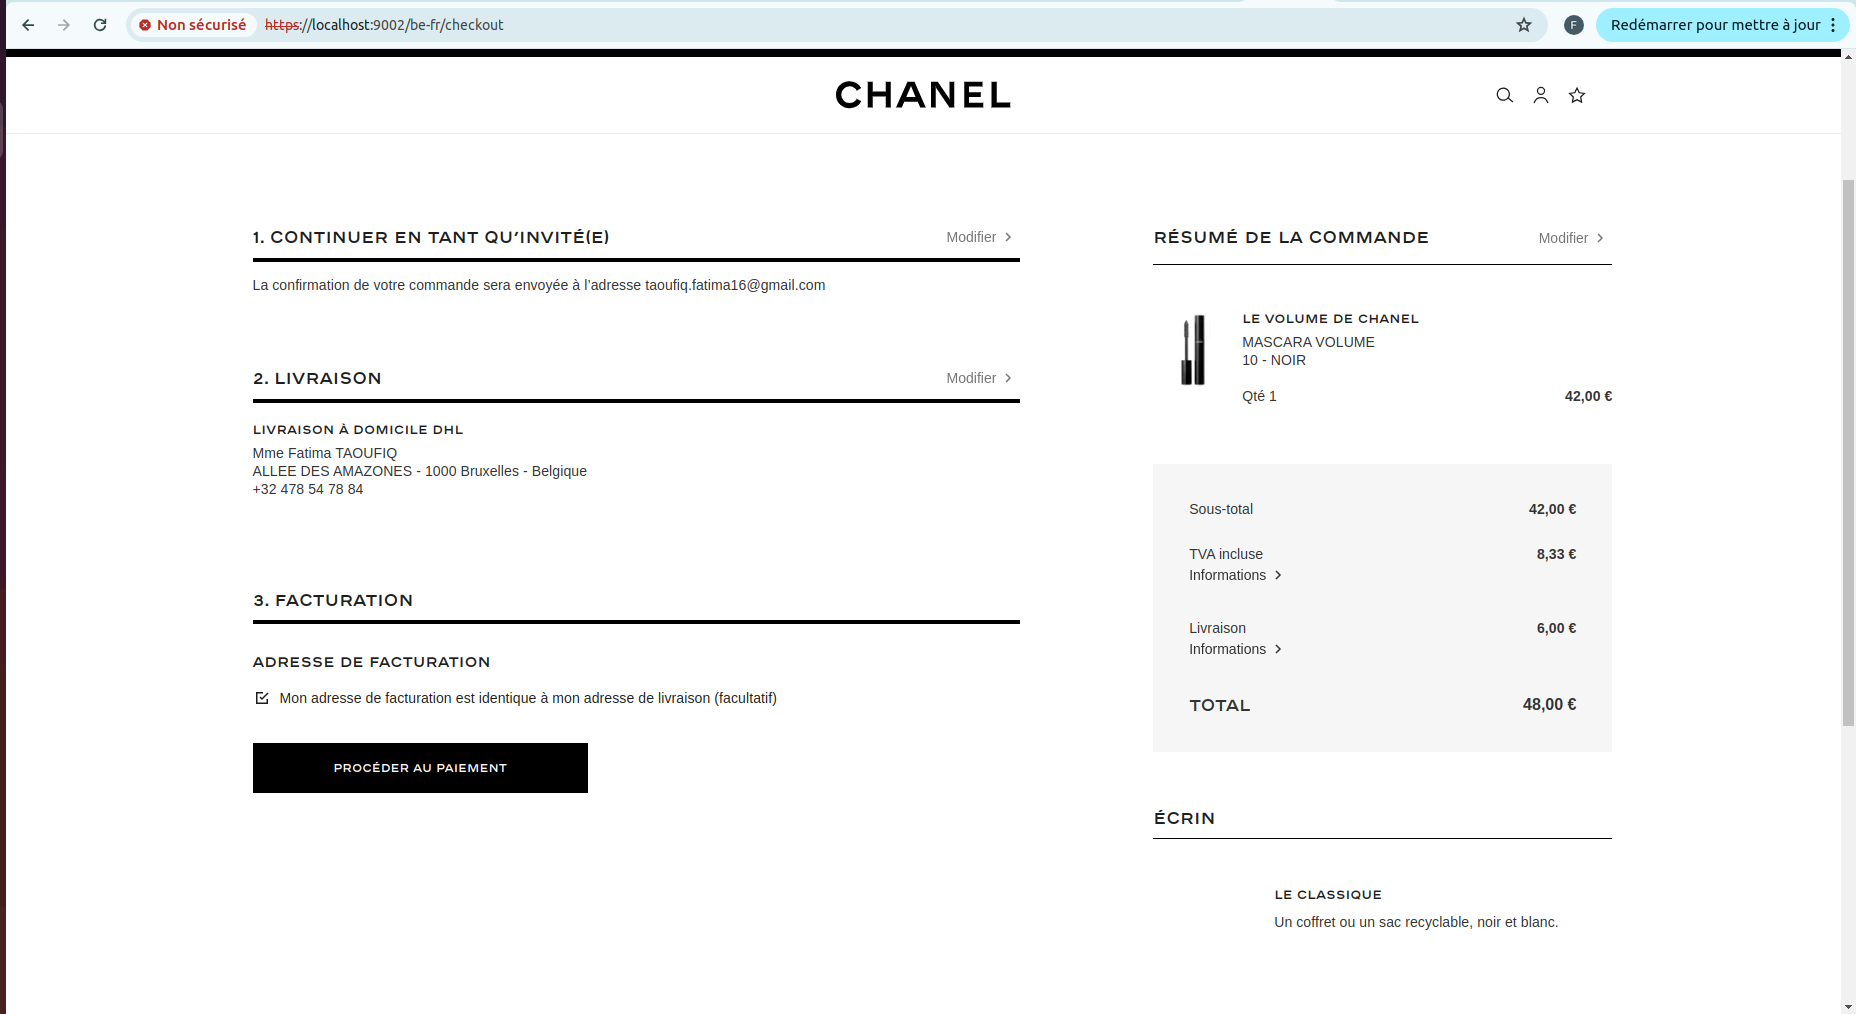
\includegraphics[width=19cm]{Figures/Screens/passe au facturation.png}
    \captionof{figure}{Facturation}
    \label{fig:facturation}
\end{center}
Après que le client a complété toutes ses informations de facturation, il accède à l'interface de sélection des modes de paiement(\textit{Figure \ref{fig:mode_paiement}}). À cette étape, il peut choisir parmi plusieurs options disponibles, y compris Payconiq, qui est mise en avant comme méthode de paiement. 
L'interface est conçue pour faciliter le choix de la méthode préférée par l'utilisateur avant de procéder à l'étape suivante du processus de paiement.
\begin{center}
    \centering
    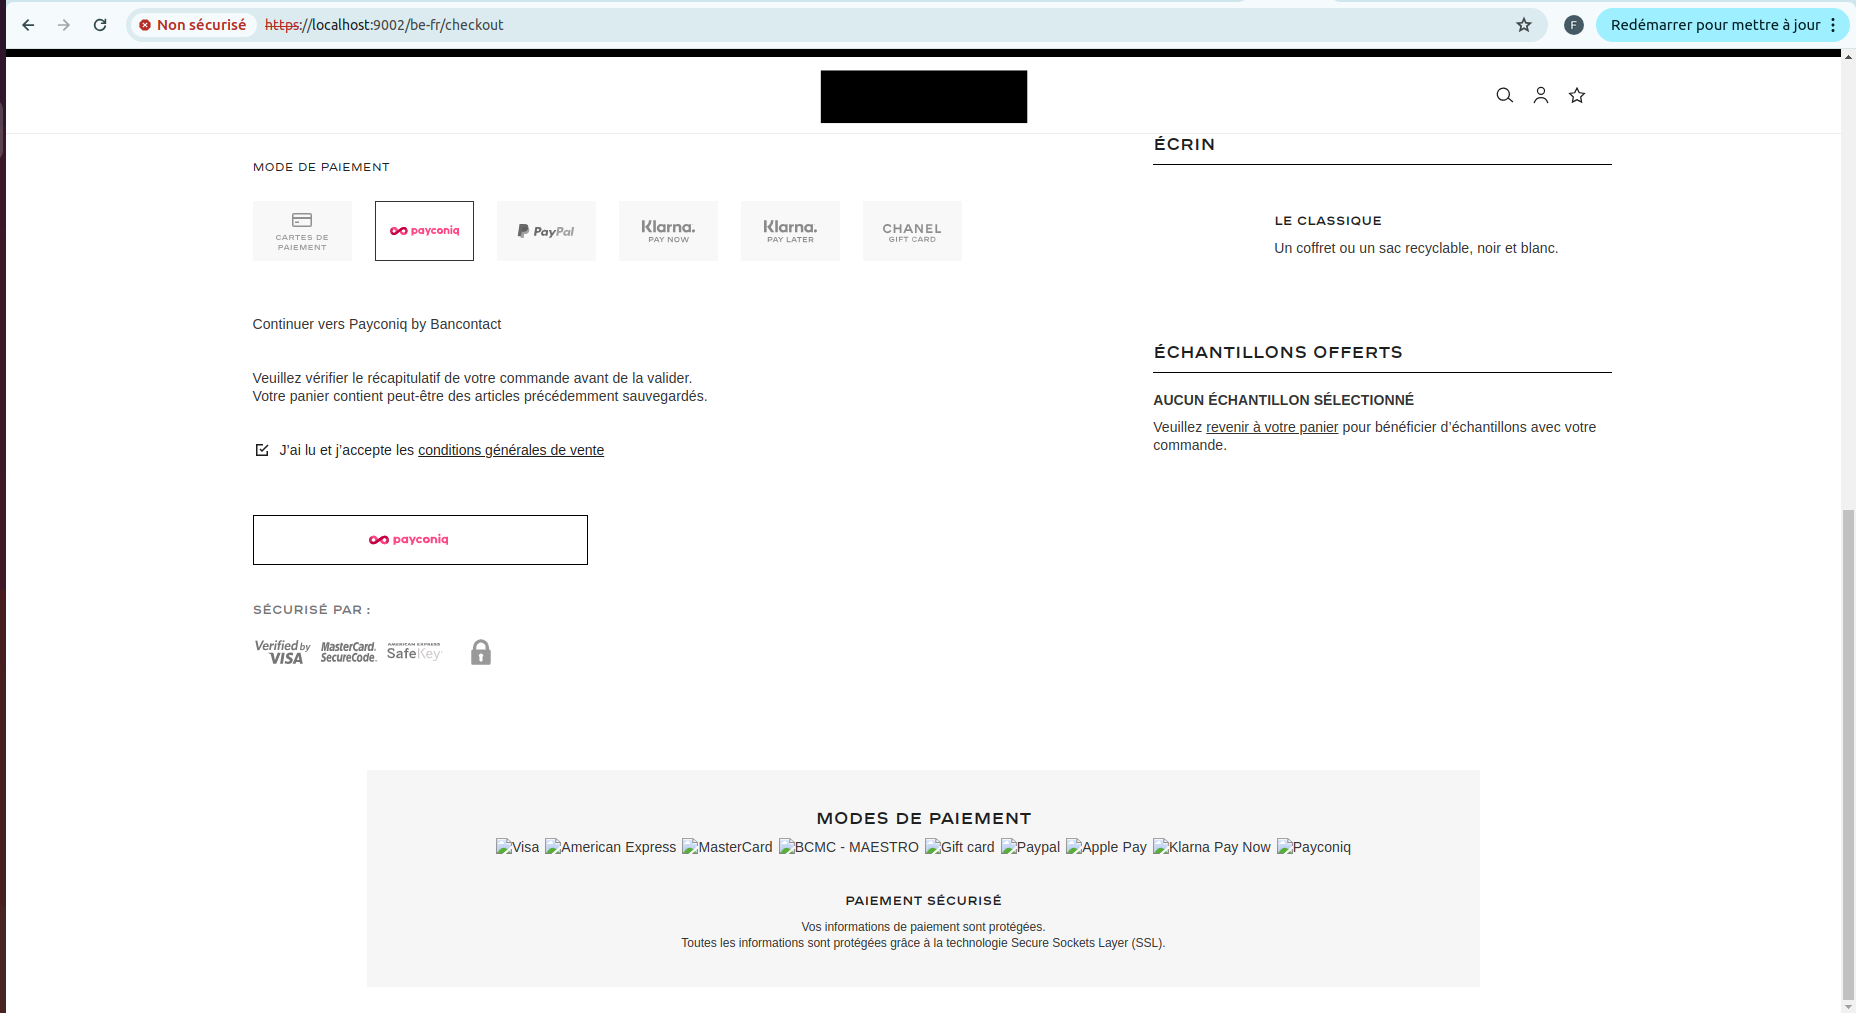
\includegraphics[width=19cm]{Figures/Screens/payment.png}
    \captionof{figure}{Choix de mode de paiement}
    \label{fig:mode_paiement}
\end{center}
Après avoir sélectionné le mode de paiement, l'utilisateur est dirigé vers l'API Adyen. Sur cette interface, un QR code est généré pour finaliser la transaction. Comme l'illustre la figure \ref{fig:qr}, ce QR code doit être scanné dans les 15 minutes pour éviter l'annulation automatique de la commande. L'interface fournit également un compte à rebours indiquant le temps restant pour effectuer le paiement, garantissant ainsi une expérience utilisateur fluide et sécurisée.
\begin{center}
    \centering
    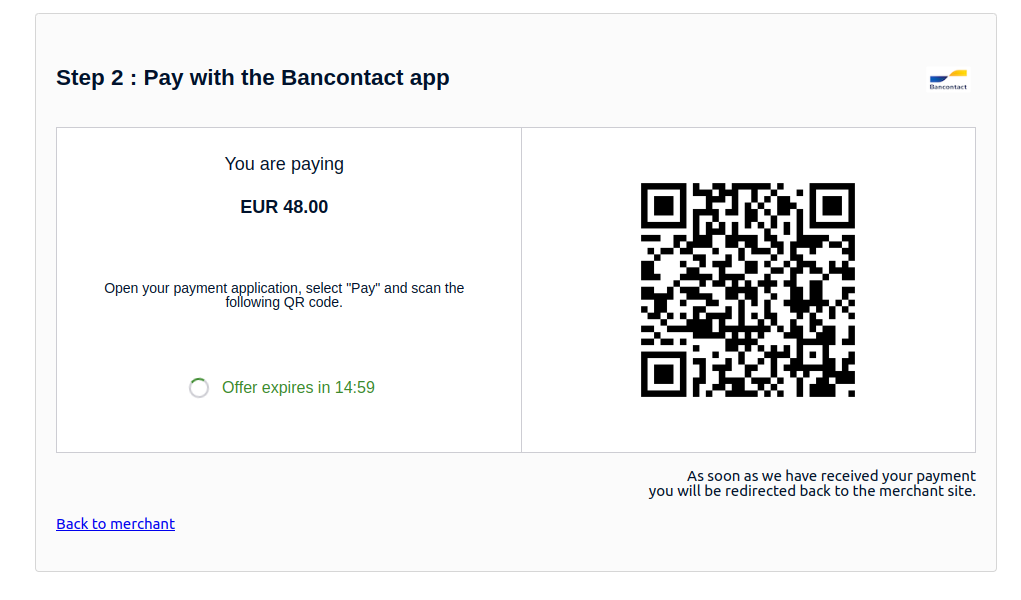
\includegraphics[width=19cm]{Figures/Screens/redirection.png}
    \captionof{figure}{Finalisation du paiement via l'API Adyen}
    \label{fig:qr}
\end{center}
Une fois redirigé vers la page de paiement, l'utilisateur traverse plusieurs étapes :
Tout d'abord, il est accueilli par un écran indiquant qu'il doit patienter pendant que la transaction est traitée. 
\begin{center}
    \centering
    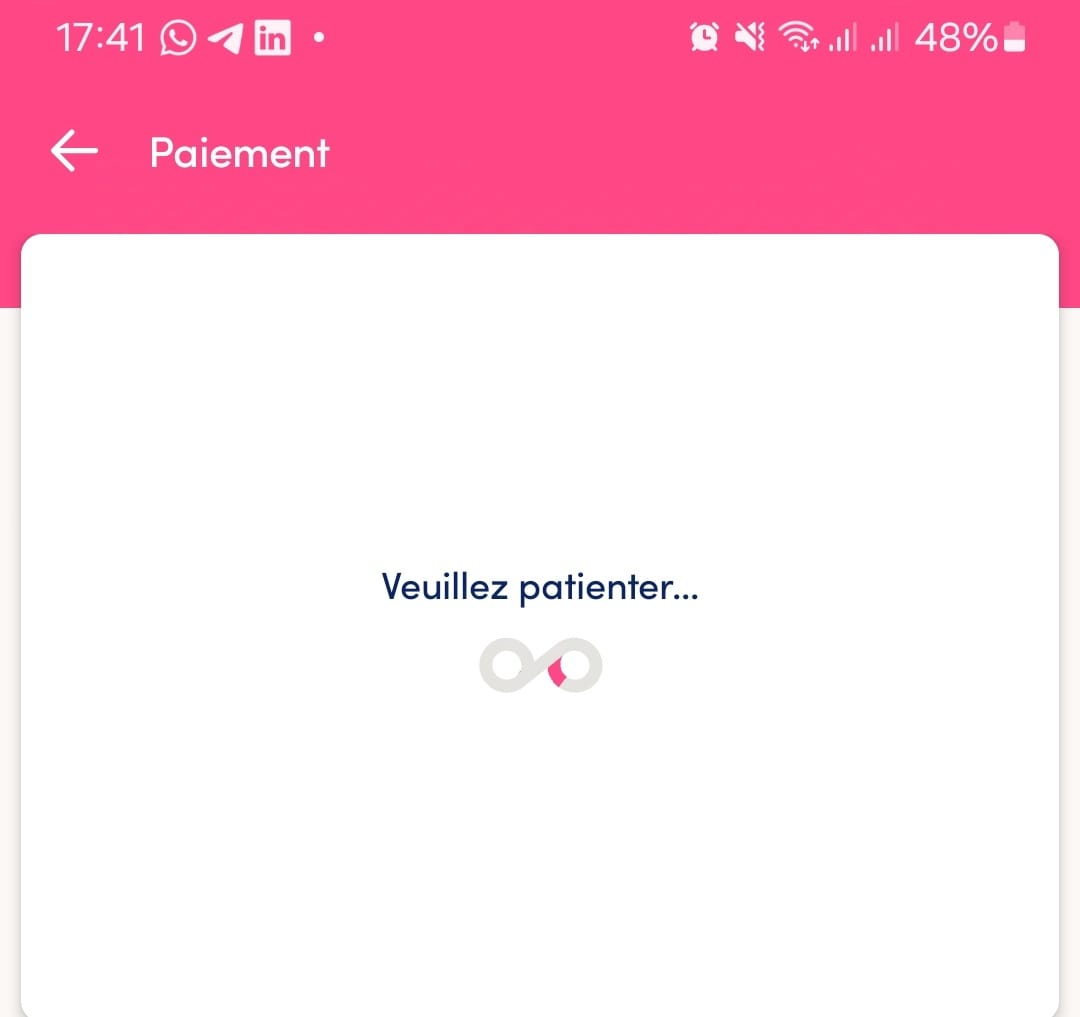
\includegraphics[width=10cm]{Figures/Screens/patience.jpeg}
    \captionof{figure}{Écran de traitement en cours}
    \label{fig:patience}
\end{center}
Ensuite, l'écran suivant affiche le montant total à payer et demande a l'utilisateur d'autoriser la transaction, comme le montre la figure \ref{fig:autorisation}
\begin{center}
    \centering
    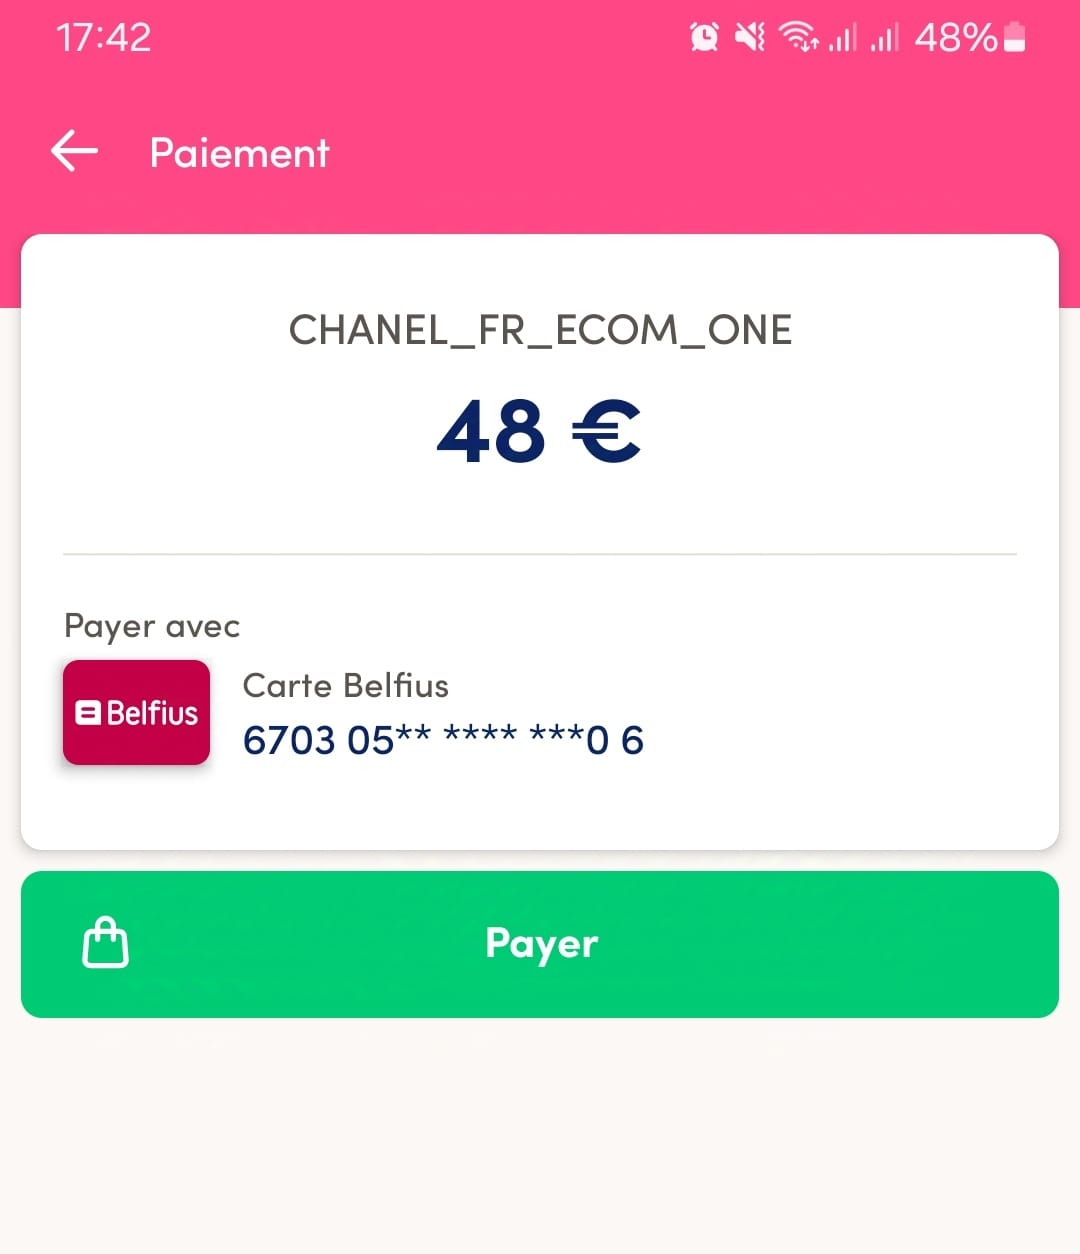
\includegraphics[width=10cm]{Figures/Screens/montant.jpeg}
    \captionof{figure}{Montant à payer}
    \label{fig:autorisation}
\end{center}
Enfin, lorsque la transaction est réussie, l'utilisateur est redirigé vers un écran de confirmation de paiement, illustré dans la figure \ref{fig:reussie}
\begin{center}
    \centering
    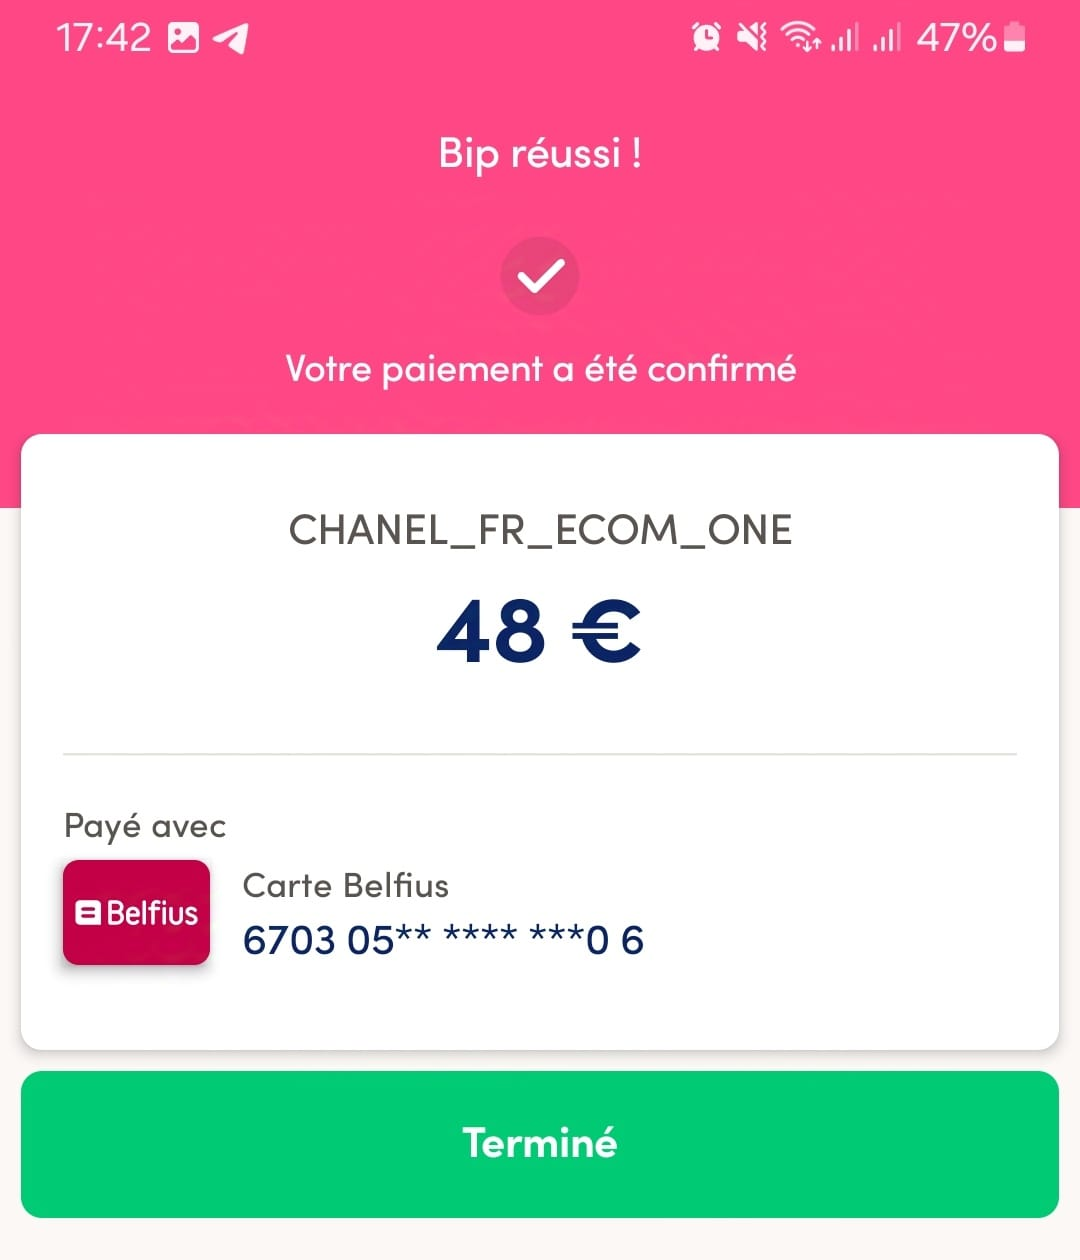
\includegraphics[width=10cm]{Figures/Screens/reussi.jpeg}
    \captionof{figure}{Paiement reussi}
    \label{fig:reussie}
\end{center}
Après la finalisation réussie du paiement, l'utilisateur est dirigé vers une page de confirmation de commande (\textit{Figure \ref{fig:confirmation}}). Cette page présente un identifiant unique de suivi, facilitant le suivi de l'état de la commande. 
\begin{center}
    \centering
    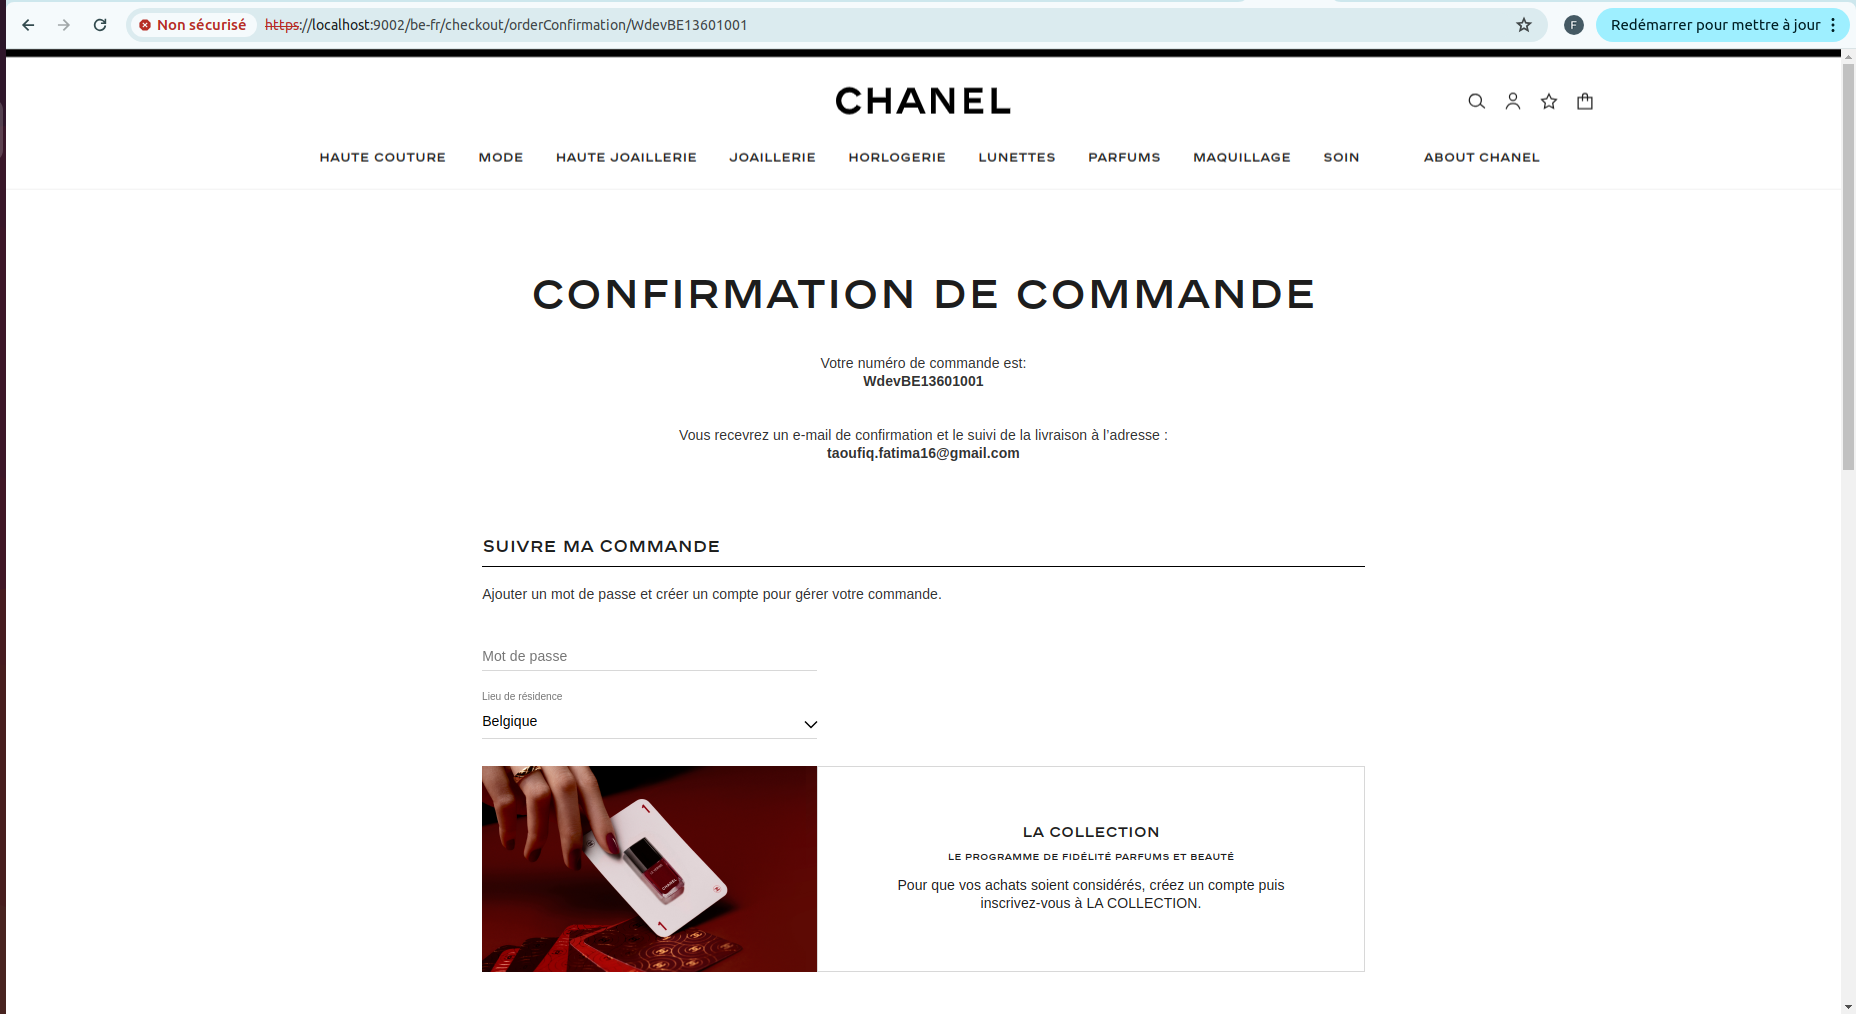
\includegraphics[width=19cm]{Figures/Screens/confirmation du commande.png}
    \captionof{figure}{Confirmation de la commande}
    \label{fig:confirmation}
\end{center}
En plus de cet identifiant, toutes les informations nécessaires sont fournies (\textit{Figure \ref{fig:resume}}), telles que l'email pour le suivi de la livraison. L'interface propose également des options pour gérer la commande, notamment la possibilité de créer un compte utilisateur pour un accès facilité aux informations de commande et aux fonctionnalités associées.
\begin{center}
    \centering
    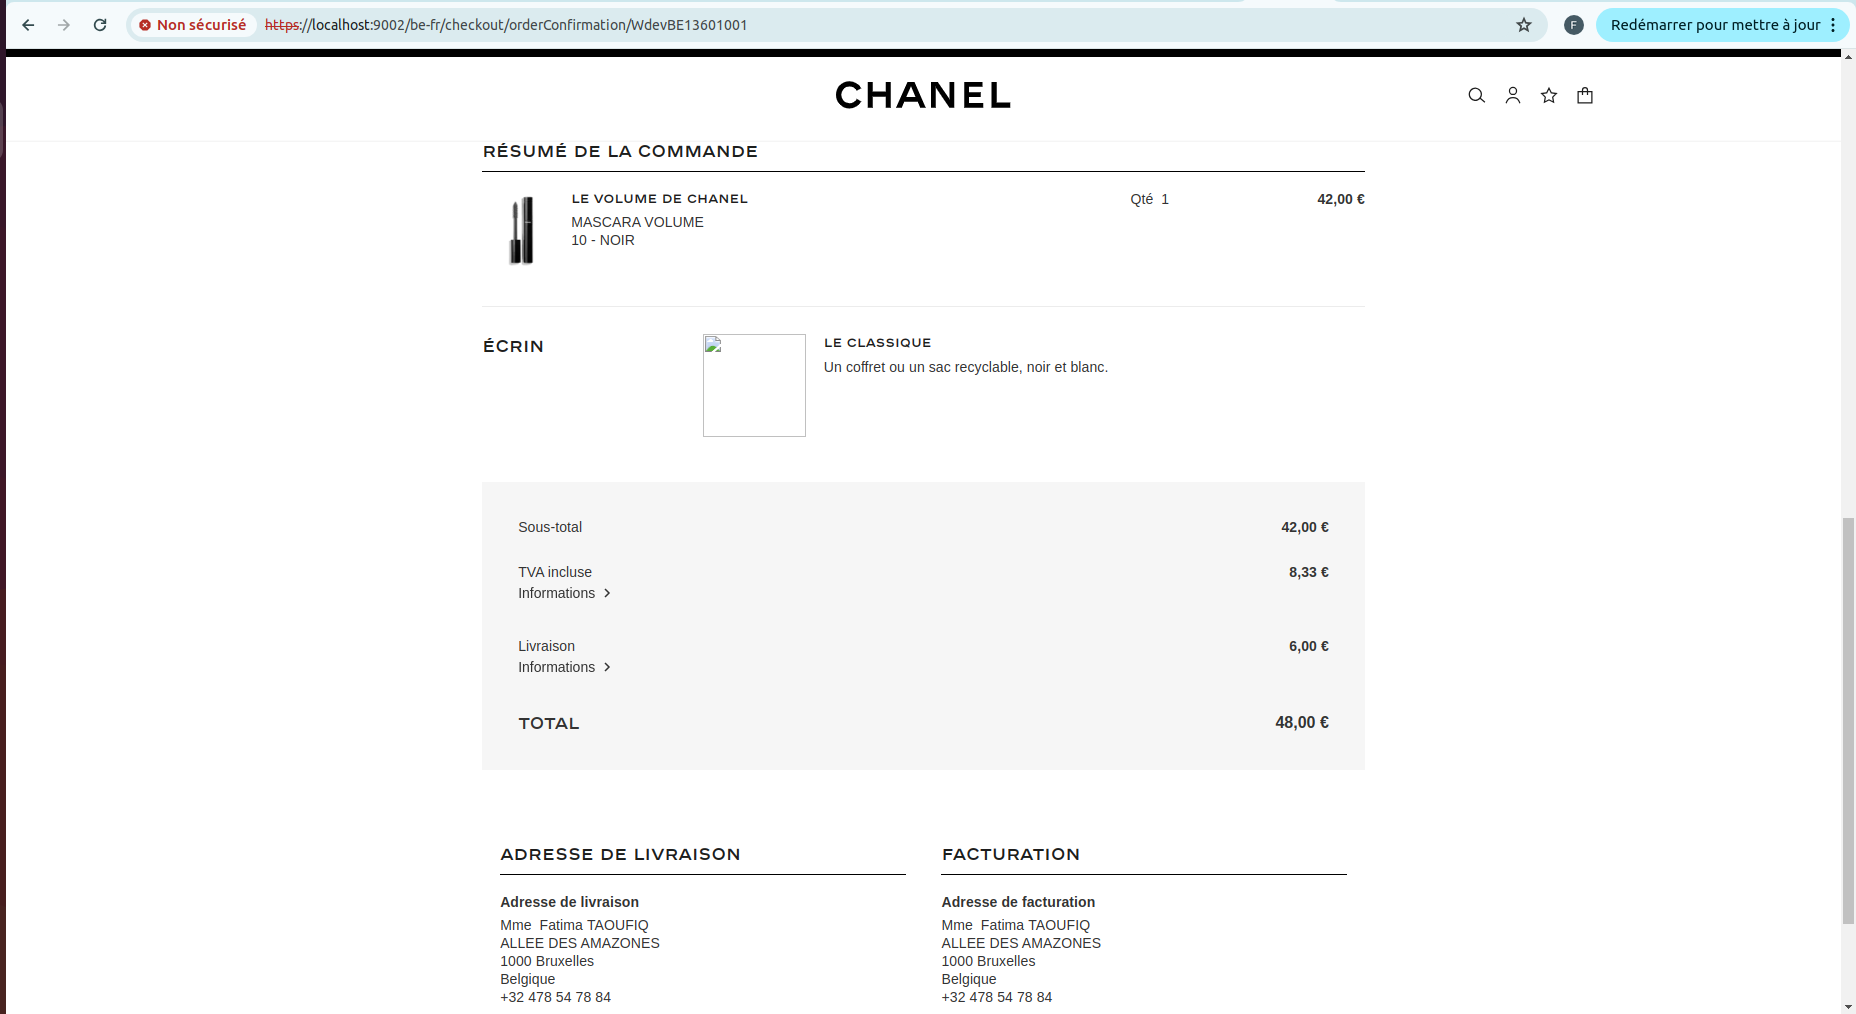
\includegraphics[width=19cm]{Figures/Screens/resumer commande.png}
    \captionof{figure}{Informations de la commande}
    \label{fig:resume}
\end{center}
En cas d'annulation ou de non-approbation du paiement, la page de confirmation de commande affichera un message d'erreur détaillé. Comme le montre la figure \ref{fig:erreur}, un avertissement est clairement indiqué : "Remarque : les informations de paiement sont erronées. Veuillez vérifier ces informations afin de confirmer votre commande." Ce message signifie que le processus de validation du paiement n'a pas été complété correctement, nécessitant une révision des informations saisies pour procéder à la confirmation de la commande.
\begin{center}
    \centering
    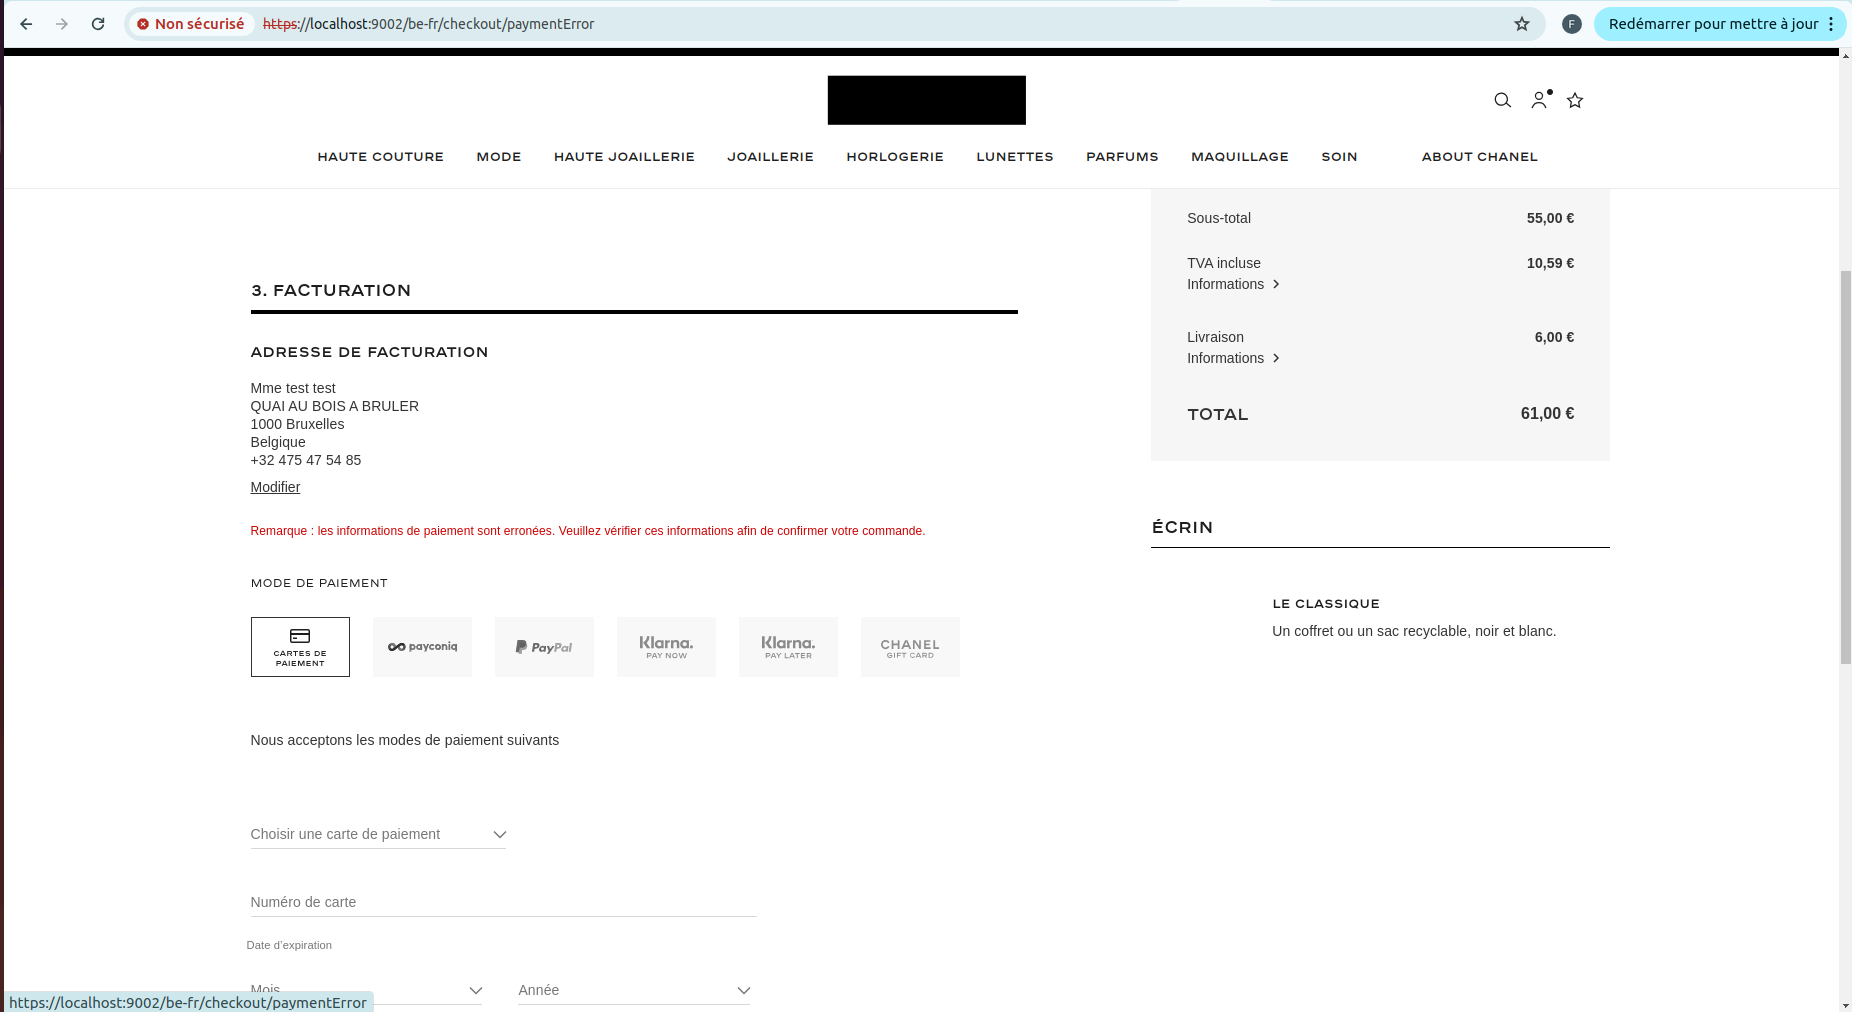
\includegraphics[width=19cm]{Figures/Screens/annulation de commande.png}
    \captionof{figure}{Message d'erreur en cas d'annulation du paiement}
    \label{fig:erreur}
\end{center}
Si la commande est effectuée avec succès, la figure \ref{fig:admin} illustre l'interface backoffice qui confirme la création de la commande et la validation réussie du paiement. Dans cet écran, l'administrateur peut consulter les détails de la commande, s'assurer que le paiement a été correctement traité et apporter toute modification nécessaire. Cette étape est essentielle pour le suivi du processus de commande et permet de gérer efficacement les commandes après l'autorisation du paiement.
\begin{center}
    \centering
    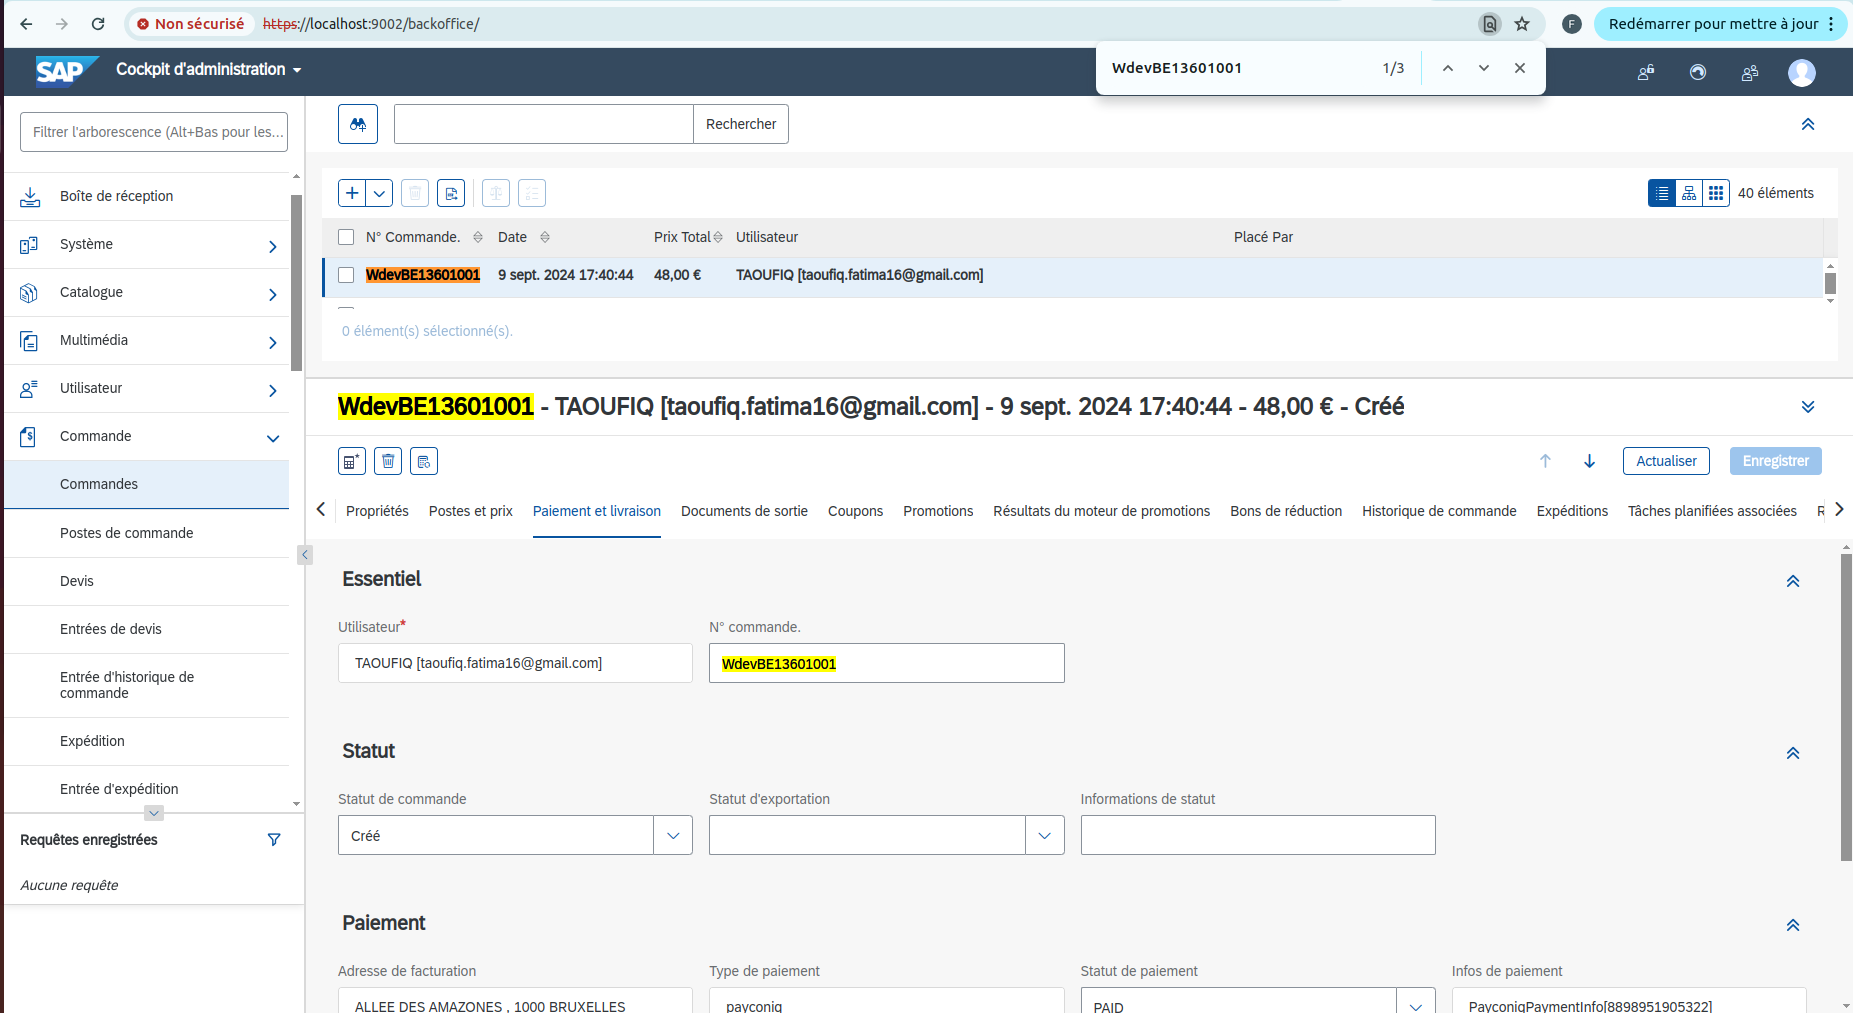
\includegraphics[width=19cm]{Figures/Screens/Backoffice commande.png}
    \captionof{figure}{Confirmation de la commande dans le backoffice}
    \label{fig:admin}
\end{center}
Une fois la commande validée, un e-mail est automatiquement envoyé à l'utilisateur, confirmant les détails de l'achat et assurant une traçabilité complète. Ce message inclut des informations essentielles telles que le numéro de commande, les articles achetés, le montant total, ainsi que les coordonnées de livraison. Cette étape permet à l'utilisateur de suivre sa commande de manière transparente et de vérifier les détails importants relatifs à son achat.
\begin{center}
    \centering
    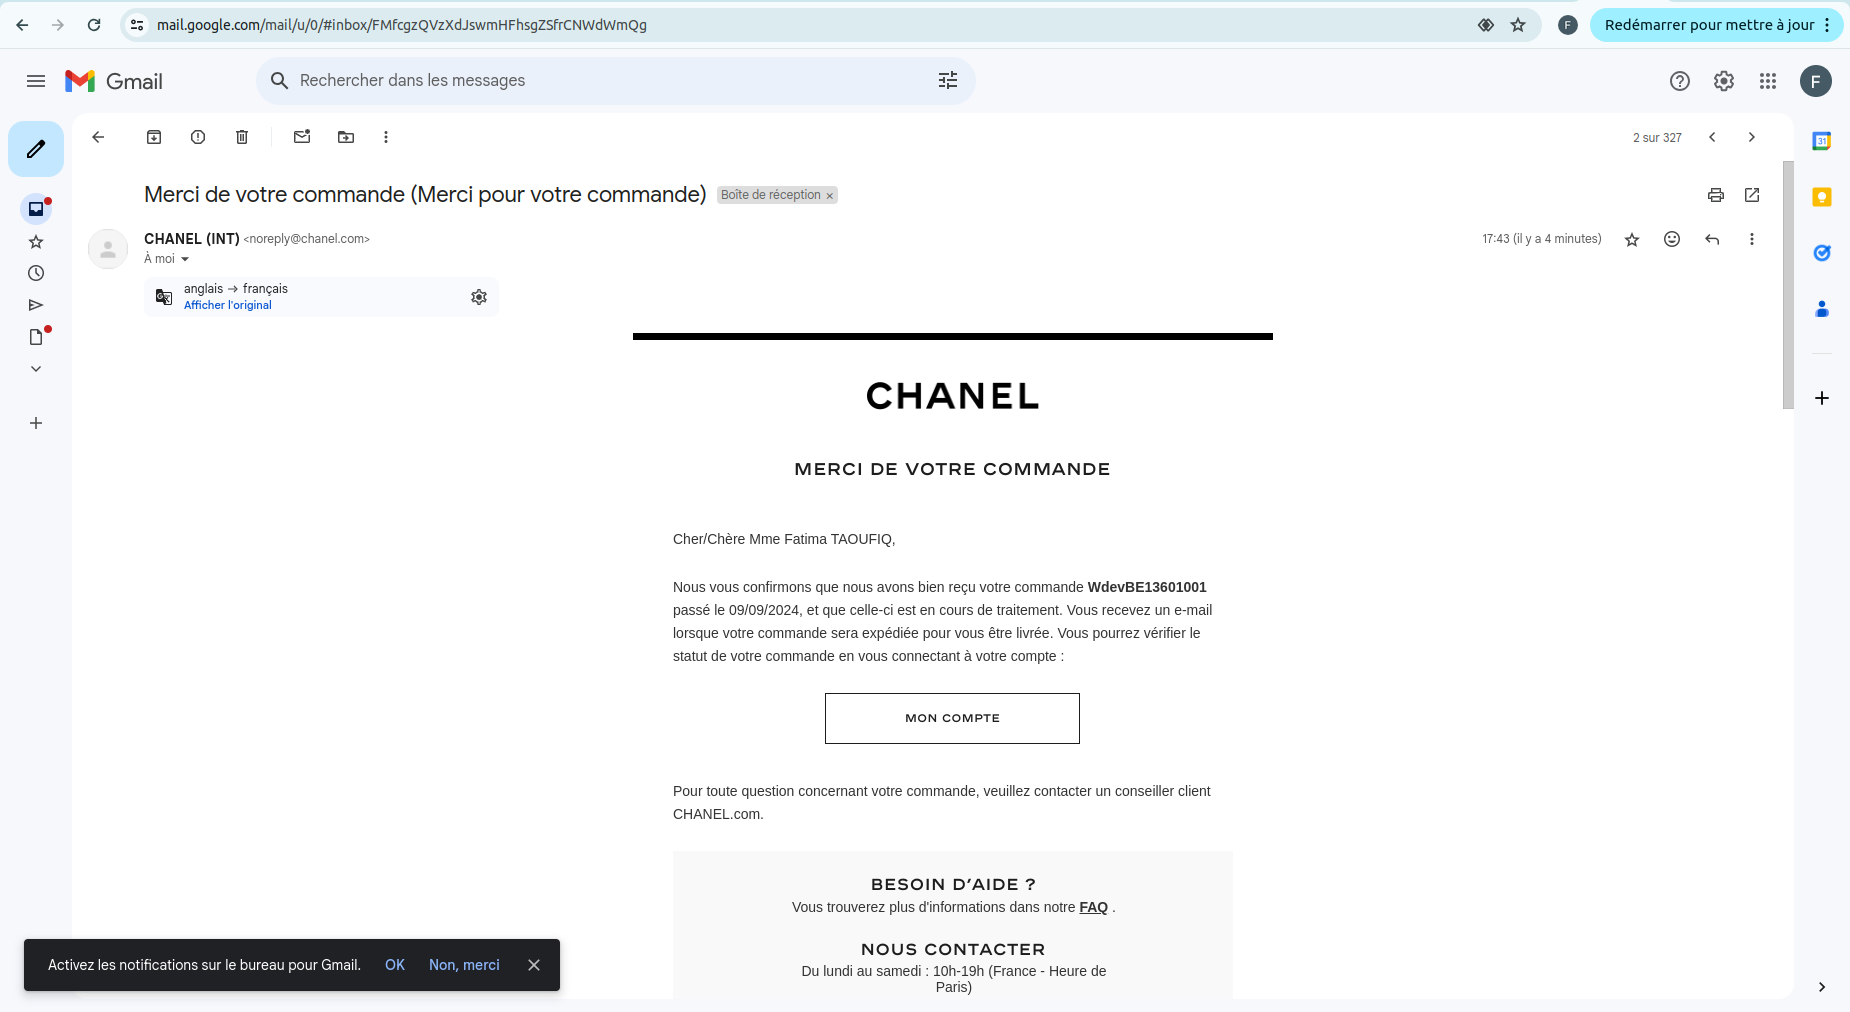
\includegraphics[width=19cm]{Figures/Screens/confirmation par mail.png}
    \captionof{figure}{Message de confirmation par email}
    \label{fig:email}
\end{center}
\section{Analyse et Correction des Anomalies}

Au cours de cette période, une partie essentielle de mon travail a consisté à résoudre les problèmes détectés par SonarQube, un outil d'analyse statique qui permet d'améliorer la qualité du code. Comme illustré par les captures ci-dessous, SonarQube a mis en évidence plusieurs anomalies critiques, notamment des  duplications de littéraux  et des  complexités cognitives  élevées dans certaines méthodes du projet. Ces problèmes, jugés critiques, nécessitaient une attention immédiate pour garantir une bonne maintenabilité du projet.

En corrigeant ces anomalies, j'ai non seulement amélioré la maintenabilité du projet, mais aussi réduit les risques d'erreurs futures. Ce travail d'optimisation a permis de renforcer la  robustesse  du code et d'assurer que le projet respecte les bonnes pratiques de développement logiciel, en ligne avec les normes de qualité du secteur.
\begin{center}
    \centering
    \includegraphics[width=19cm]{Figures/Screens/bug.png}
    \captionof{figure}{Bugs détectés par SonarQube}
    \label{fig:corr}
\end{center}
La figure \ref{fig:ticket} illustre un exemple de ticket de bug  créé pour suivre les anomalies détectées. Ce processus de gestion des bugs est essentiel pour identifier et résoudre les problèmes techniques, ce qui garantit la  stabilité  et la  qualité  du produit final. Travailler sur ces tickets a également permis de faciliter la collaboration entre les équipes, améliorant ainsi l'expérience utilisateur globale.
\begin{center}
    \centering
    \includegraphics[width=19cm]{Figures/Screens/ticket.png}
    \captionof{figure}{Exemple ticket de debugging}
    \label{fig:ticket}
\end{center}
\section{Tests et Validation}
\subsection{Tests}
Les tests constituent une étape essentielle pour s'assurer du bon fonctionnement du système et de sa conformité aux attentes. Ils aident à repérer et corriger d'éventuelles anomalies avant la mise en production. Nous avons ainsi mené différents types de tests, allant des tests unitaires aux tests fonctionnels, réalisés sur plusieurs environnements :
\begin{itemize}
    \item[$\bullet$] \textbf{Tests unitaires :} Nous avons utilisé JUnit pour mener les tests unitaires, visant à valider chaque composant du système de manière isolée. Ces tests, réalisés en local, permettent de vérifier que les méthodes fonctionnent comme prévu, de gérer les exceptions, et d’assurer la robustesse du code avant toute intégration. Grâce à une approche rigoureuse, nous avons atteint une couverture de 100\% du code, comme le montrent les captures d'écran ci-dessous. Cette couverture complète assure que chaque ligne de code a été testée et contribue à la fiabilité globale du système.
    \begin{center}
        \centering
        \includegraphics[width=18cm]{Figures/Screens/couvrage.png}
        \captionof{figure}{Couverture de code à 100\%}
        \label{fig:couvrage}
    \end{center}
    \begin{center}
        \centering
        \includegraphics[width=18cm]{Figures/Screens/reportSonar.png}
        \captionof{figure}{Succès de tous les cas de test}
        \label{fig:report}
    \end{center}
    \item[$\bullet$] \textbf{Tests fonctionnels :} Les tests fonctionnels ont été pris en charge par l'équipe QA sur plusieurs environnements, tels que INT2, INT1, UAT et OAT. Ces tests permettent de valider que les fonctionnalités développées respectent les exigences métiers et opèrent correctement dans des conditions réalistes. INT1 est utilisé comme environnement partagé par toutes les équipes, tandis que INT2 est dédié à l'équipe Cart \& Checkout Payment. Ces validations sont cruciales pour garantir la stabilité et la conformité du système avant sa mise en production.
\end{itemize}

\subsection{Validation des besoins fonctionnels}
Les besoins fonctionnels ont été validés avec succès sur l'environnement INT1. À ce stade, nous attendons la finalisation des tests dans tous les environnements pour pouvoir procéder au déploiement de la fonctionnalité en production. En parallèle, une validation finale est effectuée par le Delivery Manager afin de garantir que les objectifs fonctionnels et les exigences métiers sont entièrement satisfaits avant la mise en production.

Il est important de noter que la validation des besoins par le client est une étape cruciale qui n'a pas encore été réalisée. Nous planifions d'organiser une session de validation avec le client pour obtenir leur approbation formelle des besoins fonctionnels. Cette validation permettra de confirmer que les exigences sont bien comprises et acceptées avant le passage en production, garantissant ainsi que les attentes du client sont pleinement respectées.

\subsection{Validation des besoins non fonctionnels}
Pour garantir que le système répond aux critères essentiels de performance, il est crucial de valider les exigences non fonctionnelles définies préalablement.
\begin{itemize}
    \item[$\bullet$]\textbf{Sécurité :} La sécurité des paiements est garantie par l'utilisation de l'API d'Adyen, qui intègre des mécanismes de sécurité avancés. Adyen utilise des protocoles de cryptage de bout en bout pour protéger les données sensibles des transactions. En outre, l'API d'Adyen respecte les exigences de la directive européenne PSD2 en offrant une authentification forte du client (SCA). Cette authentification peut inclure des facteurs biométriques, des mots de passe ou des codes à usage unique, assurant ainsi une protection renforcée contre les fraudes et garantissant un niveau de sécurité optimal pour chaque transaction traitée.
    \item[$\bullet$] \textbf{Maintenabilité :} La maintenabilité du système est assurée grâce à une architecture modulaire et une documentation complète, facilitant la gestion des mises à jour et des correctifs. Les processus de déploiement automatisés minimisent les risques d'erreurs et permettent une intégration fluide des nouvelles fonctionnalités. Cette approche garantit une gestion efficace des évolutions et des corrections nécessaires au bon fonctionnement du système.
    \item[$\bullet$] \textbf{Disponibilité :} La disponibilité du système est optimisée par la configuration de déploiements répartis sur plusieurs clusters géographiques. Le projet One utilise cinq clusters situés en Amérique (AMER), en Europe, au Moyen-Orient et en Afrique (EMEA), en Asie-Pacifique, en Australie et au Canada (APAC), en Russie et en Chine. Cette répartition permet d'assurer une haute disponibilité et une résilience accrue du système, offrant une réponse rapide aux demandes des utilisateurs, indépendamment de leur emplacement. Grâce à cette architecture distribuée, le système bénéficie d'une latence réduite et d'un temps de réponse optimisé. En cas de panne d'un cluster, le trafic est automatiquement redirigé vers les autres clusters, assurant ainsi la continuité du service et minimisant les interruptions. Cette approche contribue à maintenir une expérience utilisateur fluide et efficace.
\end{itemize}

\section*{Conclusion}
Ce chapitre a été consacré à la mise en place de la solution développée. Après une brève introduction des technologies employées, les captures d'écran ont mis en lumière les fonctionnalités réalisées. Les détails des tests entrepris ont ensuite permis de valider l'efficacité de la nouvelle méthode de paiement. Ces étapes ont assuré que la plateforme répond aux exigences fonctionnelles et maintient une performance optimale.




% \chapter{General Project Context}
\label{chap:General Project Context}

% "*" makes the section unnumbered

\section*{Introduction}

Use this template as you wish, change what you want to change, the section titles are only examples, you don't have to follow them to the letter.


This is an example of me citing the 1st reference in the bibliography at the end of this report \cite{ref1}. Use it well!

The next section contains the README text that's also found in the left part along with the other files.


\newpage

\section{READ\_ME}

Hi! 

This template is a combination of multiple student and teacher PFE report templates that I have compiled into one that hopefully will satisfy your needs.
\\

It is in English, but I have included the french "Page de garde" if you want to use it, and the rest of the paper is easily translatable.
\\

This document is compiled using pdfLatex Compiler, so make sure you select it in the menu on the top left of the page. You can change the font size there along with other things.
\\

Some table, figure, list or formatting codes can be found in the "Codes\_needed.tex" file in this same folder, use them well.
\\

The organisation of this template is as follows: 
\\
The main compilation file is main.tex, any file you want to add, should be added there using, %\chapter{General Project Context}
\label{chap:General Project Context}

% "*" makes the section unnumbered

\section*{Introduction}

Use this template as you wish, change what you want to change, the section titles are only examples, you don't have to follow them to the letter.


This is an example of me citing the 1st reference in the bibliography at the end of this report \cite{ref1}. Use it well!

The next section contains the README text that's also found in the left part along with the other files.


\newpage

\section{READ\_ME}

Hi! 

This template is a combination of multiple student and teacher PFE report templates that I have compiled into one that hopefully will satisfy your needs.
\\

It is in English, but I have included the french "Page de garde" if you want to use it, and the rest of the paper is easily translatable.
\\

This document is compiled using pdfLatex Compiler, so make sure you select it in the menu on the top left of the page. You can change the font size there along with other things.
\\

Some table, figure, list or formatting codes can be found in the "Codes\_needed.tex" file in this same folder, use them well.
\\

The organisation of this template is as follows: 
\\
The main compilation file is main.tex, any file you want to add, should be added there using, %\chapter{General Project Context}
\label{chap:General Project Context}

% "*" makes the section unnumbered

\section*{Introduction}

Use this template as you wish, change what you want to change, the section titles are only examples, you don't have to follow them to the letter.


This is an example of me citing the 1st reference in the bibliography at the end of this report \cite{ref1}. Use it well!

The next section contains the README text that's also found in the left part along with the other files.


\newpage

\section{READ\_ME}

Hi! 

This template is a combination of multiple student and teacher PFE report templates that I have compiled into one that hopefully will satisfy your needs.
\\

It is in English, but I have included the french "Page de garde" if you want to use it, and the rest of the paper is easily translatable.
\\

This document is compiled using pdfLatex Compiler, so make sure you select it in the menu on the top left of the page. You can change the font size there along with other things.
\\

Some table, figure, list or formatting codes can be found in the "Codes\_needed.tex" file in this same folder, use them well.
\\

The organisation of this template is as follows: 
\\
The main compilation file is main.tex, any file you want to add, should be added there using, %\input{Chapters/Chapter1} for example. 

Remember to change the PDF Title and author name before the begin document command.
\\

Packages.tex is where you import packages and could modify their options.
\\

The frontmatter folder contains unnumbered chapters that come before the actual chapters, so the resumes and acknowledgments are there. The pages are numbered in Roman numbers.
\\

The chapters folder obviously contains the main chapters of the report, usually the first one is an intro, of both the project and the company, the last one is a conclusion chapter, I made it unnumbered here but you do you.
\\

The endmatter folder contains the appendices, acronyms, glossary, and Complementary figures, tables and codes. Consider checking this link \url{https://libguides.usc.edu/writingguide/appendices} for more info. Usually you add an appendix for each subject you'll talk about it, each with its own codes, tables, figures and text.
\\

The bibliography can be found at the end of main.tex file.
\\

And to organise your figures better, upload the logos to the logos folder, and content related figures should go in the figures folder, where you can add sub folders.
\\

Along the template, make sure to read my comments, they can be helpful to understand the purpose of a command or option. 
\\

When you finish writing your thesis, make sure to verify that you didn't leave any generic line or link. Revise it well.
\\

There are 10 warnings that show up in this template, some I couldn't manage to solve (or understand), and some I left since they are necessary for what I intend of this template.
\\

Obviously this template is only a suggestion, it is not perfect in any sense, you can improve it in the way that suits you, so search away, and get used to reading the documentation.
\\

Also consult with your supervisor, as each teacher has their own opinion on what constitutes the ideal report.
\\

Finally, I hope you have enjoyed your time at INPT as much as I did, and Good Luck :D
\\

-Mery


\subsection{Codes\_Needed}

This subsection includes codes for different elements you will need: figures, tables, lists...

Copy the codes you want and test them in the chapter files.

if you want symbols and other text styles, visit this link: 

\href{https://www.cmor-faculty.rice.edu/~heinken/latex/symbols.pdf}{Symbols}

Read the comments !!

% Content division

%\chapter{Comes first}, then \section{}, then \subsection{}, then \subsubsection{}.

\subsubsection{Text formatting}

\textbf{This text is bold}

\textit{This text is italic}

\underline{This text is underlined.}

\st{This text is struck out.}

\textsc{This text is capitalized.}

%Use \paragraph{To start a paragraph}


Some characters like "\%", "\$" and "\&" are significant in Latex code, so to include them in normal text, use the backslash character before them.
To print out backslash, use \symbol{92}


Documentation: \href{https://www.overleaf.com/learn/latex/Bold%2C_italics_and_underlining}{Italics and underlining}


\subsubsection{Figures} 

\begin{figure}[H] 
    \centering
    \includegraphics[width=4cm]{Logos/Logo_INPT.png}
    \caption{Caption}
    \label{fig:my_label} %Optional (If you want to reference the figure in later chapters)
\end{figure}

%[width=7cm] you control the size of the image. other options include: 
%[height=7cm] or [scale=0.5] (means half the size of the original image)


Documentation: \href{https://www.overleaf.com/learn/latex/Inserting_Images}{Images}


\subsubsection{Tables} 

Simple table without borders:
\\

\begin{tabular}{ll}
  First & Second \\
  Third & Fourth
\end{tabular}
\\

More complex table with borders:
\\

\begin{tabular}{|l|c|r|} \hline
  Left aligned column & Centered column & Right aligned column \\ \hline
  Text & Text & Text \\ \hline
\end{tabular}
\\

Example of a short table

%{5cm} is the cell length, you can change it to suit your own table

\begin{table}[H]
    \centering
    \begin{tabular}{|m{5cm}|m{10cm}|}
        \hline
          Column1 & Column2 \\
        \hline
          Element11 & Element21 \\
        \hline
          Element12 & Element22 \\
        \hline
          Element13 & Element23 \\
        \hline
    \end{tabular}
    \caption{Table Example}
\end{table}


Example of a long table (that spans 2 pages or more), Latex will automatically split the table when it reaches the end of the page:

\begin{longtable}[c]{| m{4.4cm} | m{11cm} |}
\caption{Long table}\\
 \hline

 Cell & Description  \\ 
 \hline
 \endfirsthead

 \hline
 
 Cell & Description  \\ 
 \hline
 \endhead

        \hline
          Element11 & Element21 \\
        \hline
          Element12 & Element22 \\
        \hline
          Element13 & Element23 \\
        \hline
          Element14 & Element24 \\
        \hline
          Element15 & Element25 \\
        \hline
          Element16 & Element26 \\
        \hline
          Element17 & Element27 \\
        \hline
          Element18 & Element28 \\
        \hline
          Element19 & Element29 \\
        \hline
          Element110 & Element210 \\
        \hline
          Element111 & Element211 \\
        \hline
          Element112 & Element212 \\
        \hline
          Element113 & Element213 \\
        \hline
          Element114 & Element214 \\
        \hline

 \end{longtable}


Documentation: \href{https://www.overleaf.com/learn/latex/Tables}{Tables}


\subsubsection{Lists}

To start an unnumbered list, use:

\begin{itemize}
    \item 
    \item 
    \item 
\end{itemize}

To start a numbered list, use:

\begin{enumerate}
    \item 
    \item 
    \item 
\end{enumerate}



Documentation: \href{https://www.overleaf.com/learn/latex/Lists}{Lists}


\subsubsection{Code scripts or terminal}

Say you have a script or terminal command you want to include, you use the following code:

    \lstset{style=mystyle} %this style is already defined in Packages.tex
    
    \begin{lstlisting}[language=bash, caption= Code caption]
    
    root@eve-ng:~# mkdir -p /opt/unetlab/addons/qemu/timos-20.10.R12

    \end{lstlisting}


Documentation: \href{https://www.overleaf.com/learn/latex/Code_listing}{Code Listing}

\subsubsection{Math}

Some math formulas for you, test them in your chapters:

These are inline formulas: $x$, $a_i^2 + b_i^2 \le a_{i+1}^2$. Afterwards...

These are centered formulas: $$x,$$ $$a_i^2 + b_i^2 \le a_{i+1}^2.$$ Afterwards...

Some complex formula: $$P(|S - E[S]| \ge t) \le 2 \exp \left( -\frac{2 t^2 n^2}{\sum_{i = 1}^n (b_i - a_i)^2} \right).$$

Also you can use the first link for math symbols and other useful stuff:

Documentation: \href{https://www.cmor-faculty.rice.edu/~heinken/latex/symbols.pdf}{Symbols file again}



\newpage


\section{Presentation of host organization}



\subsection{Company Overview}

\begin{figure}[H] 
    \centering
    \includegraphics[width=7cm]{Logos/Company_Logo_Expl.png}
    \caption{Company logo}
    %\label{fig:my_label} %Optional (If you want to reference the figure in later chapters)
\end{figure}



\subsection{Organizational Chart}


\begin{figure}[H] 
    \centering
    \includegraphics[width=12cm]{Figures/Organizational_Chart.png}
    \caption{Organizational Chart}
    %\label{fig:my_label} %Optional (If you want to reference the figure in later chapters)
\end{figure}











\section{Presentation of the project}


\subsection{Project Framework}



\subsection{Project objectives}





\subsection{Project Planning}

\begin{figure}[H] 
    \centering
    \includegraphics[width=12cm]{Figures/Gantt_Diagram.png}
    \caption{Gantt Diagram}
    %\label{fig:my_label} %Optional (If you want to reference the figure in later chapters)
\end{figure}

\newpage

\section*{Conclusion}

Lorem ipsum dolor sit amet, consectetur adipiscing elit. Praesent nec dapibus justo. Donec sagittis vulputate ante sed porttitor. Suspendisse sit amet nisl massa. Curabitur nec nisl condimentum, egestas ex vitae, dapibus enim. Etiam iaculis, erat faucibus pellentesque sagittis, nisi justo sollicitudin nibh, et condimentum augue massa non turpis. Proin commodo enim fermentum suscipit condimentum. Maecenas molestie, dui nec vestibulum rhoncus, arcu nisl faucibus neque, a ornare nisi massa ac eros. Aenean id velit sit amet lacus mattis varius. Donec fringilla massa sed nisi eleifend, a aliquet mi tempus. Nunc posuere euismod est, nec tristique augue lobortis non. Sed sodales sem ut metus tempus ullamcorper.
 for example. 

Remember to change the PDF Title and author name before the begin document command.
\\

Packages.tex is where you import packages and could modify their options.
\\

The frontmatter folder contains unnumbered chapters that come before the actual chapters, so the resumes and acknowledgments are there. The pages are numbered in Roman numbers.
\\

The chapters folder obviously contains the main chapters of the report, usually the first one is an intro, of both the project and the company, the last one is a conclusion chapter, I made it unnumbered here but you do you.
\\

The endmatter folder contains the appendices, acronyms, glossary, and Complementary figures, tables and codes. Consider checking this link \url{https://libguides.usc.edu/writingguide/appendices} for more info. Usually you add an appendix for each subject you'll talk about it, each with its own codes, tables, figures and text.
\\

The bibliography can be found at the end of main.tex file.
\\

And to organise your figures better, upload the logos to the logos folder, and content related figures should go in the figures folder, where you can add sub folders.
\\

Along the template, make sure to read my comments, they can be helpful to understand the purpose of a command or option. 
\\

When you finish writing your thesis, make sure to verify that you didn't leave any generic line or link. Revise it well.
\\

There are 10 warnings that show up in this template, some I couldn't manage to solve (or understand), and some I left since they are necessary for what I intend of this template.
\\

Obviously this template is only a suggestion, it is not perfect in any sense, you can improve it in the way that suits you, so search away, and get used to reading the documentation.
\\

Also consult with your supervisor, as each teacher has their own opinion on what constitutes the ideal report.
\\

Finally, I hope you have enjoyed your time at INPT as much as I did, and Good Luck :D
\\

-Mery


\subsection{Codes\_Needed}

This subsection includes codes for different elements you will need: figures, tables, lists...

Copy the codes you want and test them in the chapter files.

if you want symbols and other text styles, visit this link: 

\href{https://www.cmor-faculty.rice.edu/~heinken/latex/symbols.pdf}{Symbols}

Read the comments !!

% Content division

%\chapter{Comes first}, then \section{}, then \subsection{}, then \subsubsection{}.

\subsubsection{Text formatting}

\textbf{This text is bold}

\textit{This text is italic}

\underline{This text is underlined.}

\st{This text is struck out.}

\textsc{This text is capitalized.}

%Use \paragraph{To start a paragraph}


Some characters like "\%", "\$" and "\&" are significant in Latex code, so to include them in normal text, use the backslash character before them.
To print out backslash, use \symbol{92}


Documentation: \href{https://www.overleaf.com/learn/latex/Bold%2C_italics_and_underlining}{Italics and underlining}


\subsubsection{Figures} 

\begin{figure}[H] 
    \centering
    \includegraphics[width=4cm]{Logos/Logo_INPT.png}
    \caption{Caption}
    \label{fig:my_label} %Optional (If you want to reference the figure in later chapters)
\end{figure}

%[width=7cm] you control the size of the image. other options include: 
%[height=7cm] or [scale=0.5] (means half the size of the original image)


Documentation: \href{https://www.overleaf.com/learn/latex/Inserting_Images}{Images}


\subsubsection{Tables} 

Simple table without borders:
\\

\begin{tabular}{ll}
  First & Second \\
  Third & Fourth
\end{tabular}
\\

More complex table with borders:
\\

\begin{tabular}{|l|c|r|} \hline
  Left aligned column & Centered column & Right aligned column \\ \hline
  Text & Text & Text \\ \hline
\end{tabular}
\\

Example of a short table

%{5cm} is the cell length, you can change it to suit your own table

\begin{table}[H]
    \centering
    \begin{tabular}{|m{5cm}|m{10cm}|}
        \hline
          Column1 & Column2 \\
        \hline
          Element11 & Element21 \\
        \hline
          Element12 & Element22 \\
        \hline
          Element13 & Element23 \\
        \hline
    \end{tabular}
    \caption{Table Example}
\end{table}


Example of a long table (that spans 2 pages or more), Latex will automatically split the table when it reaches the end of the page:

\begin{longtable}[c]{| m{4.4cm} | m{11cm} |}
\caption{Long table}\\
 \hline

 Cell & Description  \\ 
 \hline
 \endfirsthead

 \hline
 
 Cell & Description  \\ 
 \hline
 \endhead

        \hline
          Element11 & Element21 \\
        \hline
          Element12 & Element22 \\
        \hline
          Element13 & Element23 \\
        \hline
          Element14 & Element24 \\
        \hline
          Element15 & Element25 \\
        \hline
          Element16 & Element26 \\
        \hline
          Element17 & Element27 \\
        \hline
          Element18 & Element28 \\
        \hline
          Element19 & Element29 \\
        \hline
          Element110 & Element210 \\
        \hline
          Element111 & Element211 \\
        \hline
          Element112 & Element212 \\
        \hline
          Element113 & Element213 \\
        \hline
          Element114 & Element214 \\
        \hline

 \end{longtable}


Documentation: \href{https://www.overleaf.com/learn/latex/Tables}{Tables}


\subsubsection{Lists}

To start an unnumbered list, use:

\begin{itemize}
    \item 
    \item 
    \item 
\end{itemize}

To start a numbered list, use:

\begin{enumerate}
    \item 
    \item 
    \item 
\end{enumerate}



Documentation: \href{https://www.overleaf.com/learn/latex/Lists}{Lists}


\subsubsection{Code scripts or terminal}

Say you have a script or terminal command you want to include, you use the following code:

    \lstset{style=mystyle} %this style is already defined in Packages.tex
    
    \begin{lstlisting}[language=bash, caption= Code caption]
    
    root@eve-ng:~# mkdir -p /opt/unetlab/addons/qemu/timos-20.10.R12

    \end{lstlisting}


Documentation: \href{https://www.overleaf.com/learn/latex/Code_listing}{Code Listing}

\subsubsection{Math}

Some math formulas for you, test them in your chapters:

These are inline formulas: $x$, $a_i^2 + b_i^2 \le a_{i+1}^2$. Afterwards...

These are centered formulas: $$x,$$ $$a_i^2 + b_i^2 \le a_{i+1}^2.$$ Afterwards...

Some complex formula: $$P(|S - E[S]| \ge t) \le 2 \exp \left( -\frac{2 t^2 n^2}{\sum_{i = 1}^n (b_i - a_i)^2} \right).$$

Also you can use the first link for math symbols and other useful stuff:

Documentation: \href{https://www.cmor-faculty.rice.edu/~heinken/latex/symbols.pdf}{Symbols file again}



\newpage


\section{Presentation of host organization}



\subsection{Company Overview}

\begin{figure}[H] 
    \centering
    \includegraphics[width=7cm]{Logos/Company_Logo_Expl.png}
    \caption{Company logo}
    %\label{fig:my_label} %Optional (If you want to reference the figure in later chapters)
\end{figure}



\subsection{Organizational Chart}


\begin{figure}[H] 
    \centering
    \includegraphics[width=12cm]{Figures/Organizational_Chart.png}
    \caption{Organizational Chart}
    %\label{fig:my_label} %Optional (If you want to reference the figure in later chapters)
\end{figure}











\section{Presentation of the project}


\subsection{Project Framework}



\subsection{Project objectives}





\subsection{Project Planning}

\begin{figure}[H] 
    \centering
    \includegraphics[width=12cm]{Figures/Gantt_Diagram.png}
    \caption{Gantt Diagram}
    %\label{fig:my_label} %Optional (If you want to reference the figure in later chapters)
\end{figure}

\newpage

\section*{Conclusion}

Lorem ipsum dolor sit amet, consectetur adipiscing elit. Praesent nec dapibus justo. Donec sagittis vulputate ante sed porttitor. Suspendisse sit amet nisl massa. Curabitur nec nisl condimentum, egestas ex vitae, dapibus enim. Etiam iaculis, erat faucibus pellentesque sagittis, nisi justo sollicitudin nibh, et condimentum augue massa non turpis. Proin commodo enim fermentum suscipit condimentum. Maecenas molestie, dui nec vestibulum rhoncus, arcu nisl faucibus neque, a ornare nisi massa ac eros. Aenean id velit sit amet lacus mattis varius. Donec fringilla massa sed nisi eleifend, a aliquet mi tempus. Nunc posuere euismod est, nec tristique augue lobortis non. Sed sodales sem ut metus tempus ullamcorper.
 for example. 

Remember to change the PDF Title and author name before the begin document command.
\\

Packages.tex is where you import packages and could modify their options.
\\

The frontmatter folder contains unnumbered chapters that come before the actual chapters, so the resumes and acknowledgments are there. The pages are numbered in Roman numbers.
\\

The chapters folder obviously contains the main chapters of the report, usually the first one is an intro, of both the project and the company, the last one is a conclusion chapter, I made it unnumbered here but you do you.
\\

The endmatter folder contains the appendices, acronyms, glossary, and Complementary figures, tables and codes. Consider checking this link \url{https://libguides.usc.edu/writingguide/appendices} for more info. Usually you add an appendix for each subject you'll talk about it, each with its own codes, tables, figures and text.
\\

The bibliography can be found at the end of main.tex file.
\\

And to organise your figures better, upload the logos to the logos folder, and content related figures should go in the figures folder, where you can add sub folders.
\\

Along the template, make sure to read my comments, they can be helpful to understand the purpose of a command or option. 
\\

When you finish writing your thesis, make sure to verify that you didn't leave any generic line or link. Revise it well.
\\

There are 10 warnings that show up in this template, some I couldn't manage to solve (or understand), and some I left since they are necessary for what I intend of this template.
\\

Obviously this template is only a suggestion, it is not perfect in any sense, you can improve it in the way that suits you, so search away, and get used to reading the documentation.
\\

Also consult with your supervisor, as each teacher has their own opinion on what constitutes the ideal report.
\\

Finally, I hope you have enjoyed your time at INPT as much as I did, and Good Luck :D
\\

-Mery


\subsection{Codes\_Needed}

This subsection includes codes for different elements you will need: figures, tables, lists...

Copy the codes you want and test them in the chapter files.

if you want symbols and other text styles, visit this link: 

\href{https://www.cmor-faculty.rice.edu/~heinken/latex/symbols.pdf}{Symbols}

Read the comments !!

% Content division

%\chapter{Comes first}, then \section{}, then \subsection{}, then \subsubsection{}.

\subsubsection{Text formatting}

\textbf{This text is bold}

\textit{This text is italic}

\underline{This text is underlined.}

\st{This text is struck out.}

\textsc{This text is capitalized.}

%Use \paragraph{To start a paragraph}


Some characters like "\%", "\$" and "\&" are significant in Latex code, so to include them in normal text, use the backslash character before them.
To print out backslash, use \symbol{92}


Documentation: \href{https://www.overleaf.com/learn/latex/Bold%2C_italics_and_underlining}{Italics and underlining}


\subsubsection{Figures} 

\begin{figure}[H] 
    \centering
    \includegraphics[width=4cm]{Logos/Logo_INPT.png}
    \caption{Caption}
    \label{fig:my_label} %Optional (If you want to reference the figure in later chapters)
\end{figure}

%[width=7cm] you control the size of the image. other options include: 
%[height=7cm] or [scale=0.5] (means half the size of the original image)


Documentation: \href{https://www.overleaf.com/learn/latex/Inserting_Images}{Images}


\subsubsection{Tables} 

Simple table without borders:
\\

\begin{tabular}{ll}
  First & Second \\
  Third & Fourth
\end{tabular}
\\

More complex table with borders:
\\

\begin{tabular}{|l|c|r|} \hline
  Left aligned column & Centered column & Right aligned column \\ \hline
  Text & Text & Text \\ \hline
\end{tabular}
\\

Example of a short table

%{5cm} is the cell length, you can change it to suit your own table

\begin{table}[H]
    \centering
    \begin{tabular}{|m{5cm}|m{10cm}|}
        \hline
          Column1 & Column2 \\
        \hline
          Element11 & Element21 \\
        \hline
          Element12 & Element22 \\
        \hline
          Element13 & Element23 \\
        \hline
    \end{tabular}
    \caption{Table Example}
\end{table}


Example of a long table (that spans 2 pages or more), Latex will automatically split the table when it reaches the end of the page:

\begin{longtable}[c]{| m{4.4cm} | m{11cm} |}
\caption{Long table}\\
 \hline

 Cell & Description  \\ 
 \hline
 \endfirsthead

 \hline
 
 Cell & Description  \\ 
 \hline
 \endhead

        \hline
          Element11 & Element21 \\
        \hline
          Element12 & Element22 \\
        \hline
          Element13 & Element23 \\
        \hline
          Element14 & Element24 \\
        \hline
          Element15 & Element25 \\
        \hline
          Element16 & Element26 \\
        \hline
          Element17 & Element27 \\
        \hline
          Element18 & Element28 \\
        \hline
          Element19 & Element29 \\
        \hline
          Element110 & Element210 \\
        \hline
          Element111 & Element211 \\
        \hline
          Element112 & Element212 \\
        \hline
          Element113 & Element213 \\
        \hline
          Element114 & Element214 \\
        \hline

 \end{longtable}


Documentation: \href{https://www.overleaf.com/learn/latex/Tables}{Tables}


\subsubsection{Lists}

To start an unnumbered list, use:

\begin{itemize}
    \item 
    \item 
    \item 
\end{itemize}

To start a numbered list, use:

\begin{enumerate}
    \item 
    \item 
    \item 
\end{enumerate}



Documentation: \href{https://www.overleaf.com/learn/latex/Lists}{Lists}


\subsubsection{Code scripts or terminal}

Say you have a script or terminal command you want to include, you use the following code:

    \lstset{style=mystyle} %this style is already defined in Packages.tex
    
    \begin{lstlisting}[language=bash, caption= Code caption]
    
    root@eve-ng:~# mkdir -p /opt/unetlab/addons/qemu/timos-20.10.R12

    \end{lstlisting}


Documentation: \href{https://www.overleaf.com/learn/latex/Code_listing}{Code Listing}

\subsubsection{Math}

Some math formulas for you, test them in your chapters:

These are inline formulas: $x$, $a_i^2 + b_i^2 \le a_{i+1}^2$. Afterwards...

These are centered formulas: $$x,$$ $$a_i^2 + b_i^2 \le a_{i+1}^2.$$ Afterwards...

Some complex formula: $$P(|S - E[S]| \ge t) \le 2 \exp \left( -\frac{2 t^2 n^2}{\sum_{i = 1}^n (b_i - a_i)^2} \right).$$

Also you can use the first link for math symbols and other useful stuff:

Documentation: \href{https://www.cmor-faculty.rice.edu/~heinken/latex/symbols.pdf}{Symbols file again}



\newpage


\section{Presentation of host organization}



\subsection{Company Overview}

\begin{figure}[H] 
    \centering
    \includegraphics[width=7cm]{Logos/Company_Logo_Expl.png}
    \caption{Company logo}
    %\label{fig:my_label} %Optional (If you want to reference the figure in later chapters)
\end{figure}



\subsection{Organizational Chart}


\begin{figure}[H] 
    \centering
    \includegraphics[width=12cm]{Figures/Organizational_Chart.png}
    \caption{Organizational Chart}
    %\label{fig:my_label} %Optional (If you want to reference the figure in later chapters)
\end{figure}











\section{Presentation of the project}


\subsection{Project Framework}



\subsection{Project objectives}





\subsection{Project Planning}

\begin{figure}[H] 
    \centering
    \includegraphics[width=12cm]{Figures/Gantt_Diagram.png}
    \caption{Gantt Diagram}
    %\label{fig:my_label} %Optional (If you want to reference the figure in later chapters)
\end{figure}

\newpage

\section*{Conclusion}

Lorem ipsum dolor sit amet, consectetur adipiscing elit. Praesent nec dapibus justo. Donec sagittis vulputate ante sed porttitor. Suspendisse sit amet nisl massa. Curabitur nec nisl condimentum, egestas ex vitae, dapibus enim. Etiam iaculis, erat faucibus pellentesque sagittis, nisi justo sollicitudin nibh, et condimentum augue massa non turpis. Proin commodo enim fermentum suscipit condimentum. Maecenas molestie, dui nec vestibulum rhoncus, arcu nisl faucibus neque, a ornare nisi massa ac eros. Aenean id velit sit amet lacus mattis varius. Donec fringilla massa sed nisi eleifend, a aliquet mi tempus. Nunc posuere euismod est, nec tristique augue lobortis non. Sed sodales sem ut metus tempus ullamcorper.


% \chapter{Chapter 2 title}
\label{chap:Chapter 2 title}
\section*{Introduction}


Lorem ipsum dolor sit amet, consectetur adipiscing elit. Praesent nec dapibus justo. Donec sagittis vulputate ante sed porttitor. Suspendisse sit amet nisl massa. Curabitur nec nisl condimentum, egestas ex vitae, dapibus enim. Etiam iaculis, erat faucibus pellentesque sagittis, nisi justo sollicitudin nibh, et condimentum augue massa non turpis. Proin commodo enim fermentum suscipit condimentum. Maecenas molestie, dui nec vestibulum rhoncus, arcu nisl faucibus neque, a ornare nisi massa ac eros. Aenean id velit sit amet lacus mattis varius. Donec fringilla massa sed nisi eleifend, a aliquet mi tempus. Nunc posuere euismod est, nec tristique augue lobortis non. Sed sodales sem ut metus tempus ullamcorper.


\pagebreak


\section{Section1}

\subsection{Subsection1}
\begin{longtable}[c]{| m{4.4cm} | m{11cm} |}
\caption{Long table 1}\\
 \hline

 Cell & Description  \\ 
 \hline
 \endfirsthead

 \hline
 
 Cell & Description  \\ 
 \hline
 \endhead

        \hline
          Element11 & Element21 \\
        \hline
          Element12 & Element22 \\
        \hline
          Element13 & Element23 \\
        \hline
          Element14 & Element24 \\
        \hline
          Element15 & Element25 \\
        \hline
          Element16 & Element26 \\
        \hline
          Element17 & Element27 \\
        \hline
          Element18 & Element28 \\
        \hline
          Element19 & Element29 \\
        \hline
          Element110 & Element210 \\
        \hline
          Element111 & Element211 \\
        \hline
          Element112 & Element212 \\
        \hline
          Element113 & Element213 \\
        \hline
          Element114 & Element214 \\
        \hline

 \end{longtable}

 
\subsection{Subsection2}

\subsubsection{Subsubsection1}

\subsubsection{Subsubsection2}

\paragraph{Paragraph a}

\paragraph{Paragraph b}

\section{Section2}

\subsection{Subsection1}

\subsection{Subsection2}

\subsubsection{Subsubsection1}

\subsubsection{Subsubsection2}

\paragraph{Paragraph a}

\paragraph{Paragraph b}


\newpage

\section*{Conclusion}


Lorem ipsum dolor sit amet, consectetur adipiscing elit. Praesent nec dapibus justo. Donec sagittis vulputate ante sed porttitor. Suspendisse sit amet nisl massa. Curabitur nec nisl condimentum, egestas ex vitae, dapibus enim. Etiam iaculis, erat faucibus pellentesque sagittis, nisi justo sollicitudin nibh, et condimentum augue massa non turpis. Proin commodo enim fermentum suscipit condimentum. Maecenas molestie, dui nec vestibulum rhoncus, arcu nisl faucibus neque, a ornare nisi massa ac eros. Aenean id velit sit amet lacus mattis varius. Donec fringilla massa sed nisi eleifend, a aliquet mi tempus. Nunc posuere euismod est, nec tristique augue lobortis non. Sed sodales sem ut metus tempus ullamcorper.




























% \chapter{Chapter 3 title}
\label{chap:Chapter 3 title}
\section*{Introduction}

Lorem ipsum dolor sit amet, consectetur adipiscing elit. Praesent nec dapibus justo. Donec sagittis vulputate ante sed porttitor. Suspendisse sit amet nisl massa. Curabitur nec nisl condimentum, egestas ex vitae, dapibus enim. Etiam iaculis, erat faucibus pellentesque sagittis, nisi justo sollicitudin nibh, et condimentum augue massa non turpis. Proin commodo enim fermentum suscipit condimentum. Maecenas molestie, dui nec vestibulum rhoncus, arcu nisl faucibus neque, a ornare nisi massa ac eros. Aenean id velit sit amet lacus mattis varius. Donec fringilla massa sed nisi eleifend, a aliquet mi tempus. Nunc posuere euismod est, nec tristique augue lobortis non. Sed sodales sem ut metus tempus ullamcorper.

\newpage


\section{Section1}

\subsection{Subsection1}

\begin{table}[H]
    \centering
    \begin{tabular}{|m{5cm}|m{10cm}|}
        \hline
          Column1 & Column2 \\
        \hline
          Element11 & Element21 \\
        \hline
          Element12 & Element22 \\
        \hline
          Element13 & Element23 \\
        \hline
    \end{tabular}
    \caption{Table 1}
\end{table}


\subsection{Subsection2}

\subsubsection{Subsubsection1}

\subsubsection{Subsubsection2}

\paragraph{Paragraph a}

\paragraph{Paragraph b}

\section{Section2}

\subsection{Subsection1}

\subsection{Subsection2}

\subsubsection{Subsubsection1}

\subsubsection{Subsubsection2}

\paragraph{Paragraph a}

\paragraph{Paragraph b}


\newpage

\section*{Conclusion}

Lorem ipsum dolor sit amet, consectetur adipiscing elit. Praesent nec dapibus justo. Donec sagittis vulputate ante sed porttitor. Suspendisse sit amet nisl massa. Curabitur nec nisl condimentum, egestas ex vitae, dapibus enim. Etiam iaculis, erat faucibus pellentesque sagittis, nisi justo sollicitudin nibh, et condimentum augue massa non turpis. Proin commodo enim fermentum suscipit condimentum. Maecenas molestie, dui nec vestibulum rhoncus, arcu nisl faucibus neque, a ornare nisi massa ac eros. Aenean id velit sit amet lacus mattis varius. Donec fringilla massa sed nisi eleifend, a aliquet mi tempus. Nunc posuere euismod est, nec tristique augue lobortis non. Sed sodales sem ut metus tempus ullamcorper.

\pagebreak

% \chapter{Chapter 4 title}
\label{chap:Chapter 4 title}
\section*{Introduction}

Lorem ipsum dolor sit amet, consectetur adipiscing elit. Praesent nec dapibus justo. Donec sagittis vulputate ante sed porttitor. Suspendisse sit amet nisl massa. Curabitur nec nisl condimentum, egestas ex vitae, dapibus enim. Etiam iaculis, erat faucibus pellentesque sagittis, nisi justo sollicitudin nibh, et condimentum augue massa non turpis. Proin commodo enim fermentum suscipit condimentum. Maecenas molestie, dui nec vestibulum rhoncus, arcu nisl faucibus neque, a ornare nisi massa ac eros. Aenean id velit sit amet lacus mattis varius. Donec fringilla massa sed nisi eleifend, a aliquet mi tempus. Nunc posuere euismod est, nec tristique augue lobortis non. Sed sodales sem ut metus tempus ullamcorper.
      




\pagebreak

\section{Section1}

\subsection{Subsection1}

\subsection{Subsection2}

\subsubsection{Subsubsection1}

\subsubsection{Subsubsection2}

\paragraph{Paragraph a}

\paragraph{Paragraph b}

\section{Section2}

\subsection{Subsection1}

\subsection{Subsection2}

\subsubsection{Subsubsection1}

\subsubsection{Subsubsection2}

\paragraph{Paragraph a}

\paragraph{Paragraph b}






\newpage

\section*{Conclusion}

Lorem ipsum dolor sit amet, consectetur adipiscing elit. Praesent nec dapibus justo. Donec sagittis vulputate ante sed porttitor. Suspendisse sit amet nisl massa. Curabitur nec nisl condimentum, egestas ex vitae, dapibus enim. Etiam iaculis, erat faucibus pellentesque sagittis, nisi justo sollicitudin nibh, et condimentum augue massa non turpis. Proin commodo enim fermentum suscipit condimentum. Maecenas molestie, dui nec vestibulum rhoncus, arcu nisl faucibus neque, a ornare nisi massa ac eros. Aenean id velit sit amet lacus mattis varius. Donec fringilla massa sed nisi eleifend, a aliquet mi tempus. Nunc posuere euismod est, nec tristique augue lobortis non. Sed sodales sem ut metus tempus ullamcorper.

\pagebreak

% \chapter{Chapter 5 title}
\label{chap:Chapter 5 title} 
\section*{Introduction}

Lorem ipsum dolor sit amet, consectetur adipiscing elit. Praesent nec dapibus justo. Donec sagittis vulputate ante sed porttitor. Suspendisse sit amet nisl massa. Curabitur nec nisl condimentum, egestas ex vitae, dapibus enim. Etiam iaculis, erat faucibus pellentesque sagittis, nisi justo sollicitudin nibh, et condimentum augue massa non turpis. Proin commodo enim fermentum suscipit condimentum. Maecenas molestie, dui nec vestibulum rhoncus, arcu nisl faucibus neque, a ornare nisi massa ac eros. Aenean id velit sit amet lacus mattis varius. Donec fringilla massa sed nisi eleifend, a aliquet mi tempus. Nunc posuere euismod est, nec tristique augue lobortis non. Sed sodales sem ut metus tempus ullamcorper.

\pagebreak

\section{Section1}

\subsection{Subsection1}

\subsection{Subsection2}

\subsubsection{Subsubsection1}

\subsubsection{Subsubsection2}

\paragraph{Paragraph a}

\paragraph{Paragraph b}

\section{Section2}

\subsection{Subsection1}

\subsection{Subsection2}

\subsubsection{Subsubsection1}

\subsubsection{Subsubsection2}

\paragraph{Paragraph a}

\paragraph{Paragraph b}









\newpage
\section*{Conclusion}

Lorem ipsum dolor sit amet, consectetur adipiscing elit. Praesent nec dapibus justo. Donec sagittis vulputate ante sed porttitor. Suspendisse sit amet nisl massa. Curabitur nec nisl condimentum, egestas ex vitae, dapibus enim. Etiam iaculis, erat faucibus pellentesque sagittis, nisi justo sollicitudin nibh, et condimentum augue massa non turpis. Proin commodo enim fermentum suscipit condimentum. Maecenas molestie, dui nec vestibulum rhoncus, arcu nisl faucibus neque, a ornare nisi massa ac eros. Aenean id velit sit amet lacus mattis varius. Donec fringilla massa sed nisi eleifend, a aliquet mi tempus. Nunc posuere euismod est, nec tristique augue lobortis non. Sed sodales sem ut metus tempus ullamcorper.


% \chapter*{General Conclusion and Perspectives}


% This conclusion is unnumbered, if you want it numbered, you can remove the * from above and remove the line below, so it becomes a chapter, then add sections.

\addcontentsline{toc}{chapter}{General Conclusion and Perspectives} %adds to the table of contents 

\label{chap:General Conclusion} 

Lorem ipsum dolor sit amet, consectetur adipiscing elit. Praesent nec dapibus justo. Donec sagittis vulputate ante sed porttitor. Suspendisse sit amet nisl massa. Curabitur nec nisl condimentum, egestas ex vitae, dapibus enim. Etiam iaculis, erat faucibus pellentesque sagittis, nisi justo sollicitudin nibh, et condimentum augue massa non turpis. Proin commodo enim fermentum suscipit condimentum. Maecenas molestie, dui nec vestibulum rhoncus, arcu nisl faucibus neque, a ornare nisi massa ac eros. Aenean id velit sit amet lacus mattis varius. Donec fringilla massa sed nisi eleifend, a aliquet mi tempus. Nunc posuere euismod est, nec tristique augue lobortis non. Sed sodales sem ut metus tempus ullamcorper.

Nullam fermentum id mauris suscipit varius. Quisque tristique tempor fringilla. Nam porta tincidunt orci in consectetur. Suspendisse nec sem nisi. Suspendisse potenti. Sed sodales aliquam libero, at dapibus ligula accumsan non. Quisque congue et urna a consectetur. Nullam maximus venenatis ornare. Donec in luctus urna, vel rhoncus lectus. Etiam lobortis, lacus nec gravida iaculis, magna nulla iaculis leo, quis congue nunc tortor pellentesque lorem. Sed fermentum vulputate dui, ac malesuada eros molestie sit amet. Proin fringilla elit justo, in posuere urna porttitor et. Curabitur dictum justo vitae metus pellentesque, eget feugiat sem feugiat.

Curabitur in mauris eu felis cursus auctor eget ut massa. Curabitur eleifend consectetur magna in ultrices. Etiam ut semper turpis. Morbi sed ipsum nec sem rutrum blandit sit amet vitae felis. Vestibulum vitae hendrerit diam. Aliquam pellentesque est mi, et tempus nisl laoreet in. Maecenas consequat augue a ante congue dignissim. In condimentum erat in volutpat tempus. Mauris vulputate, enim ut dignissim varius, lorem purus tristique sapien, lobortis accumsan dolor lorem quis eros. Duis vel imperdiet metus, non suscipit tortor.


%\section{Optional Section}

\appendix


% \chapter{Glossary}
\label{chap:Glossary} 


\textbf{Telnet:} Telnet is a network protocol that allows users to establish a remote terminal connection to a computer or network device over a network.\\


\textbf{SSH (Secure Shell):} SSH is a network protocol used for secure remote administration and secure file transfers.\\


\textbf{SNMP (Simple Network Management Protocol):} SNMP is a network protocol designed for managing and monitoring network devices and systems.\\


\pagebreak

\chapter*{Conclusion générale}
\addcontentsline{toc}{chapter}{Conclusion}
Ce rapport a détaillé les résultats de mon projet de fin d’études, axé sur l'amélioration d'une plateforme e-commerce en intégrant la méthode de paiement Payconiq, spécifiquement pour le marché belge. L’objectif principal de ce projet était de moderniser la plateforme en ajoutant cette méthode de paiement pour optimiser l’expérience utilisateur et répondre aux exigences locales.

Tout au long de ce projet, j’ai exploré divers aspects du développement du système, y compris la planification technique, la conception, le déploiement et les tests rigoureux. Ce projet m’a permis de mettre en pratique les connaissances et compétences acquises au cours de mes études à l'INPT, tout en découvrant de nouvelles technologies et en intégrant un environnement professionnel. Mon expérience au sein de l’équipe de développement a été particulièrement enrichissante, offrant une perspective précieuse sur le travail en milieu professionnel et la gestion de projets réels.

Pour l’avenir, plusieurs perspectives guideront le développement ultérieur de la plateforme e-commerce et l’intégration de nouvelles fonctionnalités. Les efforts futurs pourraient inclure l’optimisation continue des processus de paiement, le renforcement des mesures de sécurité et l’exploration de nouvelles méthodes de paiement adaptées à différents marchés. Ces améliorations visent à garantir que la plateforme reste compétitive, sécurisée et adaptée aux besoins des utilisateurs, tout en répondant aux évolutions du marché et des technologies.

En conclusion, ce projet a non seulement permis d'améliorer la plateforme e-commerce en intégrant Payconiq, mais a également offert une opportunité précieuse pour affiner mes compétences techniques et professionnelles. 

% \chapter{Some subject you want to expand on}
\label{chap:Some subject you want to expand on} 


You can add more appendices depending on the subjects.
%You can decide which code snippets to use in the main report and which to add here in the annex
    
    \lstset{style=mystyle} %this style is already defined in Packages.tex
    
    \begin{lstlisting}[language=bash, caption= Bash example]
    
    [root@host ~]# You can change the language and caption.

    \end{lstlisting}



    \begin{lstlisting}[language=python, caption= Python example]
    
    # Solve the quadratic equation ax**2 + bx + c = 0

    # import complex math module
    import cmath
    
    a = 1
    b = 5
    c = 6
    
    # calculate the discriminant
    d = (b**2) - (4*a*c)
    
    # find two solutions
    sol1 = (-b-cmath.sqrt(d))/(2*a)
    sol2 = (-b+cmath.sqrt(d))/(2*a)
    
    print('The solution are {0} and {1}'.format(sol1,sol2))

    \end{lstlisting}



\begin{table}[H]
    \centering
    \begin{tabular}{|m{5cm}|m{10cm}|}
        \hline
          Column1 & Column2 \\
        \hline
          Element11 & Element21 \\
        \hline
          Element12 & Element22 \\
        \hline
          Element13 & Element23 \\
        \hline
    \end{tabular}
    \caption{Table Example}
\end{table}




\begin{longtable}[c]{| m{4.4cm} | m{11cm} |}
\caption{Long table Example}\\
 \hline

 Cell & Description  \\ 
 \hline
 \endfirsthead

 \hline
 
 Cell & Description  \\ 
 \hline
 \endhead

        \hline
          Element11 & Element21 \\
        \hline
          Element12 & Element22 \\
        \hline
          Element13 & Element23 \\
        \hline
          Element14 & Element24 \\
        \hline
          Element15 & Element25 \\
        \hline
          Element16 & Element26 \\
        \hline
          Element17 & Element27 \\
        \hline
          Element18 & Element28 \\
        \hline
          Element19 & Element29 \\
        \hline
          Element110 & Element210 \\
        \hline
          Element111 & Element211 \\
        \hline
          Element112 & Element212 \\
        \hline
          Element113 & Element213 \\
        \hline
          Element114 & Element214 \\
        \hline

 \end{longtable}



\renewcommand{\bibname}{Références}

\addcontentsline{toc}{chapter}{Références}
\begin{thebibliography}{99}
    \bibitem{SQLI}
    \emph{SQLI},\\
    \href{https://www.sqli.com/ma-fr}{\textbf{https://www.sqli.com/ma-fr}}
    
    \bibitem{valeurSQLI}
    \emph{les valeurs du groupe SQLI },\\
    \href{https://www.sqli.com/ma-fr/carriere/les-valeurs-sqli}{\textbf{https://www.sqli.com/ma-fr/carriere/les-valeurs-sqli}}
    
    \bibitem{Belge}
    \emph{Utilisateur de Payconiq}, \\
    \href{https://assets-eu-01.kc-usercontent.com/331a0185-e26c-01d0-41e9-c42bc79a1d2c/6bf42db6-6363-4041-b9d3-54c6548f8e14/Press%20Release-22Feb2024.pdf}{\textbf{https://assets-eu-01.kc-usercontent.com/331a0185-e26c-01d0-41e9-c42bc79a1d2c/6bf42db6-6363-4041-b9d3-54c6548f8e14/Press\%20Release-22Feb2024.pdf}}

    \bibitem{Payconic}
    \emph{ Justification de l’intégration de Bancontact by Payconiq},\\
    \href{https://www.payconiq.be/fr/professionnel/pourquoi-choisir-payconiq}{\textbf{https://www.payconiq.be/fr/professionnel/pourquoi-choisir-payconiq}}

    \bibitem{SAP}
    \emph{SAP},\\
    \href{https://help.sap.com/docs/}{\textbf{https://help.sap.com/docs/}}

    \bibitem{JEE} 
    \emph{JEE}, \\
    \href{https://www.neosoft.fr/nos-publications/blog-tech/les-bases-de-la-securite-en-developpement-java-ee/}{\textbf{https://www.neosoft.fr/nos-publications/blog-tech/les-bases-de-la-securite-en-developpement-java-ee/}}
   

    \bibitem{spring} 
    \emph{Spring Framework Documentation}, \\
    \href{https://docs.spring.io/spring-framework/reference/index.html}{\textbf{https://docs.spring.io/spring-framework/reference/index.html}}

    \bibitem{sonarqube} 
    \emph{SonarQube Documentation}, \\
    \href{https://docs.sonarsource.com/sonarqube/latest/}{\textbf{https://docs.sonarsource.com/sonarqube/latest/}}

    \bibitem{ant} 
    \emph{Apache Ant Manual}, \\
    \href{https://ant.apache.org/manual/index.html}{\textbf{https://ant.apache.org/manual/index.html}}

    \bibitem{junit} 
    \emph{JUnit 4 Documentation}, \\
    \href{https://junit.org/junit4/javadoc/latest/}{\textbf{https://junit.org/junit4/javadoc/latest/}}

    %  %the link is a documentation of the basic bibliography method (that    I'm using here) + bibTex which is more advanced, read it well and decide which one works best for you.
    %  \bibitem{UML}
    %  \emph{Qu'est-ce que le langage UML },
    %  \href{https://www.lucidchart.com/pages/fr/langage-uml}{\textbf{https://www.lucidchart.com/pages/fr/langage-uml}}
     
    %  \bibitem{Typescript}
    %  \emph{TypeScript pour les Programmeurs JavaScript},
    %  \href{https://www.typescriptlang.org/fr/docs/handbook/typescript-in-5-minutes.html}{\textbf{document}}
     
    %  \bibitem{VS}
    %  \emph{Visual Studio },
    %  \href{https://code.visualstudio.com/}{\textbf{https://code.visualstudio.com/}}
     
    %  \bibitem{Postman}
    %  \emph{Postman },
    %  \href{https ://www.postman.com}{\textbf{https ://www.postman.com}}
     
    %  \bibitem{GitLab}
    %  \emph{GitLab},
    %  \href{https://about.gitlab.com/}{\textbf{https://about.gitlab.com/}}
     
    %  \bibitem{StarUml}
    %  \emph{StarUML},
    %  \href{https://inf1410.teluq.ca/teluqDownload.php?file=2014/01/INF1410-PresentationStarUML.pdf}{\textbf{Document}}
     

    %  \bibitem{axios}
    %  \emph{Axios},
    %  \href{https://axios-http.com/fr/docs/intro}{\textbf{https://axios-http.com/fr/docs/intro}}
     
    \end{thebibliography}

% \begin{thebibliography}{99}
% \addcontentsline{toc}{chapter}{Bibliography}


% \bibitem{ref1}
% Author name, Book name.

% \bibitem{ref2}
% \emph{Title 1},
% \href{https://www.overleaf.com/learn/latex/Bibliography_management_with_bibtex}{\textbf{Title 2}}

%  %the link is a documentation of the basic bibliography method (that    I'm using here) + bibTex which is more advanced, read it well and decide which one works best for you.



% \end{thebibliography}

\end{document}